%% 
%DIF LATEXDIFF DIFFERENCE FILE
%DIF LATEXDIFF DIFFERENCE FILE (manuscript_submitted/main.tex vs Overleaf 3c379fa = round 9c, with its \textcolor{blue}{} revision wrappers stripped (404) and whitespace-only lines inside display math removed (4); latexdiff 1.4.0 --math-markup=whole; tables, figures, algorithms and longtables as whole blocks; post-processed: \emergencystretch, 38 references to removed labels print the label in brackets). Regenerated after round 10 with manuscript_review/make_marked_copy.py.
%DIF DEL sub.tex           Thu Nov 12 15:06:33 2026
%DIF ADD rev_nocolor.tex   Thu Nov 12 15:08:12 2026
%% Copyright 2007-2024 Elsevier Ltd
%% 
%% This file is part of the 'Elsarticle Bundle'.
%% ---------------------------------------------
%% 
%% It may be distributed under the conditions of the LaTeX Project Public
%% License, either version 1.3 of this license or (at your option) any
%% later version.  The latest version of this license is in
%%    http://www.latex-project.org/lppl.txt
%% and version 1.3 or later is part of all distributions of LaTeX
%% version 1999/12/01 or later.
%% 
%% The list of all files belonging to the 'Elsarticle Bundle' is
%% given in the file `manifest.txt'.
%% 
%% Template article for Elsevier's document class `elsarticle'
%% with numbered style bibliographic references
%% SP 2008/03/01
%% $Id: elsarticle-template-num.tex 249 2024-04-06 10:51:24Z rishi $
%%
\documentclass[preprint,12pt]{elsarticle}

%% Use the option review to obtain double line spacing
%% \documentclass[authoryear,preprint,review,12pt]{elsarticle}

%% Use the options 1p,twocolumn; 3p; 3p,twocolumn; 5p; or 5p,twocolumn
%% for a journal layout:
%% \documentclass[final,1p,times]{elsarticle}
%% \documentclass[final,1p,times,twocolumn]{elsarticle}
%% \documentclass[final,3p,times]{elsarticle}
%% \documentclass[final,3p,times,twocolumn]{elsarticle}
%% \documentclass[final,5p,times]{elsarticle}
%% \documentclass[final,5p,times,twocolumn]{elsarticle}

%% For including figures, graphicx.sty has been loaded in
%% elsarticle.cls. If you prefer to use the old commands
%% please give \usepackage{epsfig}

%% The amssymb package provides various useful mathematical symbols
\usepackage{amssymb}
%% The amsmath package provides various useful equation environments.
\usepackage{amsmath}
%% The amsthm package provides extended theorem environments
%% \usepackage{amsthm}

%% The lineno packages adds line numbers. Start line numbering with
%% \begin{linenumbers}, end it with \end{linenumbers}. Or switch it on
%% for the whole article with \linenumbers.
%% \usepackage{lineno}

\usepackage[ruled,vlined]{algorithm2e}
\usepackage{booktabs}
\usepackage{subcaption}
\usepackage{eurosym}
\usepackage{pdflscape}
\usepackage{tabularx}
%DIF 58a58-60
\usepackage{longtable} %DIF > 
\usepackage{needspace} %DIF > 
\usepackage{xcolor} %DIF > 
%DIF -------

\journal{Journal of Energy Storage}
%DIF PREAMBLE EXTENSION ADDED BY LATEXDIFF
%DIF UNDERLINE PREAMBLE %DIF PREAMBLE
\RequirePackage[normalem]{ulem} %DIF PREAMBLE
\RequirePackage{color}\definecolor{RED}{rgb}{1,0,0}\definecolor{BLUE}{rgb}{0,0,1} %DIF PREAMBLE
\providecommand{\DIFadd}[1]{{\protect\color{blue}\uwave{#1}}} %DIF PREAMBLE
\providecommand{\DIFdel}[1]{{\protect\color{red}\sout{#1}}} %DIF PREAMBLE
%DIF SAFE PREAMBLE %DIF PREAMBLE
\providecommand{\DIFaddbegin}{} %DIF PREAMBLE
\providecommand{\DIFaddend}{} %DIF PREAMBLE
\providecommand{\DIFdelbegin}{} %DIF PREAMBLE
\providecommand{\DIFdelend}{} %DIF PREAMBLE
\providecommand{\DIFmodbegin}{} %DIF PREAMBLE
\providecommand{\DIFmodend}{} %DIF PREAMBLE
%DIF FLOATSAFE PREAMBLE %DIF PREAMBLE
\providecommand{\DIFaddFL}[1]{\DIFadd{#1}} %DIF PREAMBLE
\providecommand{\DIFdelFL}[1]{\DIFdel{#1}} %DIF PREAMBLE
\providecommand{\DIFaddbeginFL}{} %DIF PREAMBLE
\providecommand{\DIFaddendFL}{} %DIF PREAMBLE
\providecommand{\DIFdelbeginFL}{} %DIF PREAMBLE
\providecommand{\DIFdelendFL}{} %DIF PREAMBLE
%DIF AMSMATHULEM PREAMBLE %DIF PREAMBLE
\makeatletter %DIF PREAMBLE
\let\sout@orig\sout %DIF PREAMBLE
\renewcommand{\sout}[1]{\ifmmode\text{\sout@orig{\ensuremath{#1}}}\else\sout@orig{#1}\fi} %DIF PREAMBLE
\makeatother %DIF PREAMBLE
%DIF COLORLISTINGS PREAMBLE %DIF PREAMBLE
\RequirePackage{listings} %DIF PREAMBLE
\RequirePackage{color} %DIF PREAMBLE
\lstdefinelanguage{DIFcode}{ %DIF PREAMBLE
%DIF DIFCODE_UNDERLINE %DIF PREAMBLE
  moredelim=[il][\color{red}\sout]{\%DIF\ <\ }, %DIF PREAMBLE
  moredelim=[il][\color{blue}\uwave]{\%DIF\ >\ } %DIF PREAMBLE
} %DIF PREAMBLE
\lstdefinestyle{DIFverbatimstyle}{ %DIF PREAMBLE
	language=DIFcode, %DIF PREAMBLE
	basicstyle=\ttfamily, %DIF PREAMBLE
	columns=fullflexible, %DIF PREAMBLE
	keepspaces=true %DIF PREAMBLE
} %DIF PREAMBLE
\lstnewenvironment{DIFverbatim}[1][]{\lstset{style=DIFverbatimstyle}}{} %DIF PREAMBLE
\lstnewenvironment{DIFverbatim*}[1][]{\lstset{style=DIFverbatimstyle,showspaces=true}}{} %DIF PREAMBLE
\lstset{extendedchars=\true,inputencoding=utf8}

%DIF END PREAMBLE EXTENSION ADDED BY LATEXDIFF

\begin{document}
\sloppy % marked copy only: long marked lines

\begin{frontmatter}

%% Title, authors and addresses

%% use the tnoteref command within \title for footnotes;
%% use the tnotetext command for theassociated footnote;
%% use the fnref command within \author or \affiliation for footnotes;
%% use the fntext command for theassociated footnote;
%% use the corref command within \author for corresponding author footnotes;
%% use the cortext command for theassociated footnote;
%% use the ead command for the email address,
%% and the form \ead[url] for the home page:
%% \title{Title\tnoteref{label1}}
%% \tnotetext[label1]{}
%% \author{Name\corref{cor1}\fnref{label2}}
%% \ead{email address}
%% \ead[url]{home page}
%% \fntext[label2]{}
%% \cortext[cor1]{}
%% \affiliation{organization={},
%%             addressline={},
%%             city={},
%%             postcode={},
%%             state={},
%%             country={}}
%% \fntext[label3]{}

\title{Degradation-Aware Planning of Shared Battery Energy Storage Systems for Coordinated Transmission and Distribution System Operation}

%% use optional labels to link authors explicitly to addresses:
%% \author[label1,label2]{}
%% \affiliation[label1]{organization={},
%%             addressline={},
%%             city={},
%%             postcode={},
%%             state={},
%%             country={}}
%%
%% \affiliation[label2]{organization={},
%%             addressline={},
%%             city={},
%%             postcode={},
%%             state={},
%%             country={}}

\author[inesctec,feup_ses]{Micael Simões}
\author[inesctec,feup_dee,feup_ses]{João Peças Lopes}
\author[inesctec,feup_dee]{Filipe Joel Soares}

\affiliation[inesctec]{organization={INESC TEC, Center for Power and Energy Systems},
            addressline={Campus da Faculdade de Engenharia da Universidade do Porto, Rua Dr. Roberto Frias}, 
            city={Porto},
            postcode={4200-465}, 
            state={Porto},
            country={Portugal}}

\affiliation[feup_dee]{organization={FEUP, Department of Electrical and Computer Engineering},
            addressline={Rua Dr. Roberto Frias}, 
            city={Porto},
            postcode={4200-465}, 
            state={Porto},
            country={Portugal}}

\affiliation[feup_ses]{organization={FEUP, Sustainable Energy Systems},
            addressline={Rua Dr. Roberto Frias}, 
            city={Porto},
            postcode={4200-465}, 
            state={Porto},
            country={Portugal}}


% ====================================================================================================================
%                                                       ABSTRACT                                                      
% ====================================================================================================================
\begin{abstract}
    \DIFaddbegin \begingroup
    \emergencystretch=2em

        \DIFadd{Shared }\DIFaddend Energy Storage Systems (ESSs) \DIFdelbegin \DIFdel{are an important source of flexibility in power systems with high penetration of Renewable Energy Sources (RESs). When }\DIFdelend installed at transmission--distribution interface nodes \DIFdelbegin \DIFdel{, shared ESSs }\DIFdelend can support both Transmission System Operators (TSOs) and Distribution System Operators (DSOs)\DIFdelbegin \DIFdel{, but their long-term planning remains challenging because investment decisions depend on }\DIFdelend \DIFaddbegin \DIFadd{. Their planning must account for }\DIFaddend coordinated operation under uncertainty and battery degradation\DIFdelbegin \DIFdel{over time}\DIFdelend .
        This paper proposes a degradation-aware \DIFdelbegin \DIFdel{planning framework for shared battery ESSs in coordinated TSO--DSO operation. The problem is }\DIFdelend \DIFaddbegin \DIFadd{framework for the siting, sizing and installation year of shared lithium-ion battery ESSs, }\DIFaddend formulated as a \DIFdelbegin \DIFdel{bi-level stochastic optimization model in which the upper level determines siting, sizing, and staged investment decisions under investment-cost uncertainty, while the lower level evaluates these decisions through coordinated system operation. To preserve tractability, the framework combines Benders' decomposition for long-term planning with }\DIFdelend \DIFaddbegin \DIFadd{two-stage stochastic program in which one scenario-independent plan is evaluated under coordinated operation; uncertainty in future converter and battery investment costs enters as probability-weighted cost trajectories. A derivative-free search explores discrete investment plans in a single operating scenario, }\DIFaddend an Alternating Direction Method of Multipliers (ADMM)-based \DIFdelbegin \DIFdel{decentralized coordination mechanism for short-term operation.
    }\DIFdelend \DIFaddbegin \DIFadd{coordination procedure evaluates their operation, and fixed plans are then re-evaluated under load, renewable-generation and market-price scenarios. Battery degradation links storage dispatch with available energy capacity over the planning horizon, and numerical acceptance criteria assess the stability of operating-cost comparisons.
        }\DIFaddend The framework is evaluated on \DIFdelbegin \DIFdel{integrated IEEE }\DIFdelend \DIFaddbegin \DIFadd{an integrated 108-bus }\DIFaddend transmission--distribution test system\DIFdelbegin \DIFdel{s}\DIFdelend  over a 15-year \DIFdelbegin \DIFdel{planning horizon. Relative to uncoordinated operation, coordinated operation with shared ESSs reduces }\DIFdelend \DIFaddbegin \DIFadd{horizon. Without shared storage, coordination reduces discounted }\DIFaddend operating costs by \DIFdelbegin \DIFdel{up to 18.25\% and RES curtailment by up to 92.16\% in the later years of the planning horizon, while eliminating voltage violations. The results also show that degradation materially affects ESS valuation and that temporal discretization can influence siting and sizing decisions. }\DIFdelend \DIFaddbegin \DIFadd{12.2\% relative to a price-taker benchmark that prohibits reverse active-power flow from distribution to transmission. Under the baseline assumptions, none of the evaluated storage plans recovers its investment cost. For a fixed reference 0.25~MVA/1~MWh unit, baseline ageing yields an investment shortfall of 64.4~k}\euro{}\DIFadd{, while the margin without ageing is within numerical resolution of break-even. The unit achieves positive investment margins at 1.75 and 2 times the base flexibility price. Its estimated margin remains negative in the $3 \times 3$ multi-scenario evaluation.
    }

    \par
    \endgroup
\DIFaddend \end{abstract}


%%Graphical abstract
% ====================================================================================================================
%                                                  GRAPHICAL ABSTRACT                                                 
% ====================================================================================================================
\begin{graphicalabstract}
    \DIFdelbegin %DIFDELCMD < \includegraphics[width=1.00\textwidth]{framework.pdf}
%DIFDELCMD < %%%
\DIFdelend \DIFaddbegin \includegraphics[width=1.00\textwidth]{framework_v3.pdf}
\DIFaddend \end{graphicalabstract}


\begin{highlights}
    \item A \DIFdelbegin \DIFdel{bi-level stochastic framework is proposed for planning shared ESSs }\DIFdelend \DIFaddbegin \DIFadd{two-stage framework plans shared lithium-ion storage }\DIFaddend at TN--DN interface nodes
    \item \DIFdelbegin \DIFdel{Cycling-induced battery degradation is explicitly linked to coordinated multi-year TSO--DSO operation
    }\DIFdelend \DIFaddbegin \DIFadd{Battery degradation links storage dispatch with long-term available capacity
    }\DIFaddend \item \DIFdelbegin \DIFdel{Benders' decomposition and ADMM enable scalable planning with decentralized AC-feasible operation
    }\DIFdelend \DIFaddbegin \DIFadd{No evaluated storage plan recovers its investment cost under baseline assumptions
    }\DIFaddend \item \DIFdelbegin \DIFdel{Shared ESSs reduce operating costs, RES curtailment, and voltage violations under coordinated operation
    }\DIFdelend \DIFaddbegin \DIFadd{Reference unit margins are positive at 1.75 and 2 times the base flexibility price
    }\DIFaddend \item \DIFdelbegin \DIFdel{Planning-horizon discretization materially affects degradation trajectories and ESS investment decisions
}\DIFdelend \DIFaddbegin \DIFadd{Coordination without storage cuts operating costs by 12.2\% versus price-taking
}\DIFaddend \end{highlights}


\begin{keyword}
    Shared energy storage systems \sep
    Battery degradation \sep
    \DIFdelbegin \DIFdel{Bi-level stochastic optimization }\DIFdelend \DIFaddbegin \DIFadd{Two-stage stochastic programming }\DIFaddend \sep
    TSO--DSO coordination \sep
    \DIFdelbegin \DIFdel{Benders' decomposition }\DIFdelend \DIFaddbegin \DIFadd{Derivative-free optimization }\DIFaddend \sep
    ADMM
\end{keyword}


\end{frontmatter}

%% Add \usepackage{lineno} before \begin{document} and uncomment 
%% following line to enable line numbers
%% \linenumbers

% ====================================================================================================================
%                                                     NOMENCLATURE                                                    
% ====================================================================================================================
\DIFaddbegin 

\DIFaddend \section*{Nomenclature}

\DIFaddbegin \Needspace{6\baselineskip}
\DIFaddend \subsection*{Sets and \DIFdelbegin \DIFdel{Parameters}\DIFdelend \DIFaddbegin \DIFadd{Indices}\DIFaddend }

\DIFdelbegin %DIFDELCMD < \begin{table}[htbp!]
%DIFDELCMD <     \centering
%DIFDELCMD <     \begin{tabular}{l l}
%DIFDELCMD <         \toprule
%DIFDELCMD <         \textbf{Symbol} & \textbf{Description} \\
%DIFDELCMD <         \midrule    
%DIFDELCMD <         \multicolumn{2}{l}{\textbf{Sets}}\\
%DIFDELCMD <         $E^S$       & Set of shared ESSs \\
%DIFDELCMD <         $Y$         & Set of representative years \\
%DIFDELCMD <         $D$         & Set of representative days \\
%DIFDELCMD <         $T$         & Set of intra-day time instants \\
%DIFDELCMD <         $\Omega_C$  & Set of investment-cost scenarios \\     
%DIFDELCMD <         $L^B$       & Set of Benders' iterations\\
%DIFDELCMD <         \midrule
%DIFDELCMD <         \multicolumn{2}{l}{\textbf{Parameters}}\\
%DIFDELCMD <         $\omega_c$ & Probability of investment-cost scenario $c \in \Omega_C$ \\
%DIFDELCMD <         $c^{\text{Inv,S}}_{y,c}$ & Unit investment cost of converter power rating in year $y$ and \\
%DIFDELCMD <         ~                        & investment scenario $c$\\
%DIFDELCMD <         $c^{\text{Inv,E}}_{y,c}$ & Unit investment cost of energy capacity in year $y$ and \\
%DIFDELCMD <         ~                        & investment scenario $c$\\        
%DIFDELCMD <         $T^\text{Cal}_{e,y}$ & Calendar lifetime of ESS $e$ installed in year $y$ \\
%DIFDELCMD <         $E^{\text{Max}}_{e,y}$ & Maximum installable energy capacity of unit $e$ in year $y$ \\
%DIFDELCMD <         $\phi^{\text{Min}}_e$ & Minimum admissible energy-to-power ratio of unit $e$ in year $y$ \\
%DIFDELCMD <         $\phi^{\text{Max}}_e$ & Maximum admissible energy-to-power ratio of unit $e$ in year $y$ \\
%DIFDELCMD <         $c^{\text{Inv}}$ & Total investment budget \\
%DIFDELCMD <         $\alpha^{\text{Down}}$ & Lower bound on the Benders underestimator \\
%DIFDELCMD <         $SoH_{e,y}^{\text{min}}$ & Minimum admissible SoH of unit $e$ in year $y$ \\
%DIFDELCMD <         $D_d$ & Number of calendar days represented by $d \in D$ \\
%DIFDELCMD <         $Y_y$ & Number of calendar years represented by $y \in Y$ \\
%DIFDELCMD <         $\mathrm{CL}^\text{Nom}_e$ & Nominal cycle life of unit $e \in E^S$\\
%DIFDELCMD <         $r$   & Discount rate\\      
%DIFDELCMD <         \bottomrule
%DIFDELCMD <     \end{tabular}
%DIFDELCMD < \end{table}
%DIFDELCMD < %%%
\DIFdelend \DIFaddbegin \begingroup
    \footnotesize
    \setlength{\LTpre}{0pt}
    \setlength{\LTpost}{0pt}
    \begin{longtable}{@{}>{\raggedright\arraybackslash}p{0.29\textwidth} >{\raggedright\arraybackslash}p{\dimexpr0.71\textwidth-2\tabcolsep\relax}@{}}
        \toprule
        \textbf{Symbol} & \textbf{Description} \\
        \midrule
        \endhead
        \midrule
        \endfoot
        \bottomrule
        \endlastfoot
        $E^S$       & Set of candidate shared-ESS locations at TN–DN interface nodes, indexed by $e$ \\
        $Y$         & Set of representative years, indexed by $y$ \\
        $D$         & Set of representative days, indexed by $d$ \\
        $T$         & Set of intra-day time intervals, indexed by $t$ \\
        $\Omega_C$  & Set of investment-cost trajectories, indexed by $c$ \\
        $\Omega_M$  & Set of market scenarios, indexed by $m$ \\
        $\Omega_O$  & Set of operation scenarios (load, RES), indexed by $o$ \\
        $\Omega$ & Set of joint market and operation scenarios, $\Omega=\Omega_M\times\Omega_O$ \\     
        $\mathcal{X}$ & Set of admissible investment plans \\
        $\mathcal{U}_s(\boldsymbol{x})$ & Feasible set of operational decisions under scenario $s$ for plan $\boldsymbol{x}$ \\
        $y^{\text{Inv}}$ & Investment year \\
        $s = (m,o)$ & Recourse scenario (market and operation pair) \\
        $\mathcal{Y}^{\text{Act}}_{e,y}$ & Set of installation years of cohorts active at node $e$ in representative year $y$ \\
        $i$, $a$ & DN index; agent index (TSO, DSOs, shared-ESS agent) \\
    \end{longtable}
    \addtocounter{table}{-1}
\endgroup
\DIFaddend 

\DIFaddbegin \Needspace{6\baselineskip}
\DIFaddend \subsection*{\DIFdelbegin \DIFdel{Variables}\DIFdelend \DIFaddbegin \DIFadd{Parameters}\DIFaddend }

\DIFdelbegin %DIFDELCMD < \begin{table}[htbp!]
%DIFDELCMD <     \centering
%DIFDELCMD <     \begin{tabular}{l l}
%DIFDELCMD <         \toprule
%DIFDELCMD <         \textbf{Variable} & \textbf{Description} \\
%DIFDELCMD <         \midrule
%DIFDELCMD <         $S^{\text{Inv}(l)}_{e,y,c}$ & Scenario-dependent investment in converter power rating in \\
%DIFDELCMD <         ~                           & ESS $e$ in year $y$ and investment scenario $c$\\
%DIFDELCMD <         $E^{\text{Inv}(l)}_{e,y,c}$ & Scenario-dependent investment in energy capacity in ESS $e$ \\
%DIFDELCMD <         ~                           & in year $y$ and investment scenario $c$\\
%DIFDELCMD <         $S^{\text{Rated}}_{e,y^\text{Inv},y}$   & Rated power of unit $e$ installed in year $y^\text{Inv}$ \\
%DIFDELCMD <         ~                                       & and operated in year $y$ \\
%DIFDELCMD <         $E^{\text{Rated}}_{e,y^\text{Inv},y}$ & Available energy capacity of unit $e$ installed in year $y^\text{Inv}$\\
%DIFDELCMD <         ~                                       & and operated in year $y$ \\
%DIFDELCMD <         $S^{\text{Av,Unit}}_{e,y^\text{Inv},y}$ & Available power of unit $e$ installed in year $y^\text{Inv}$ \\
%DIFDELCMD <         ~                                       & and operated in year $y$ \\
%DIFDELCMD <         $E^{\text{Av,Unit}}_{e,y^\text{Inv},y}$ & Available energy capacity of unit $e$ installed in year $y^\text{Inv}$\\
%DIFDELCMD <         ~                                       & and operated in year $y$ \\
%DIFDELCMD <         $SoH_{e,y^\text{Inv},y}$ & SoH of unit $e$ installed in year $y^\text{Inv}$ and operated in year $y$ \\
%DIFDELCMD <         $\delta_{e,y^\text{Inv},y}$ & Average equivalent daily degradation rate of unit $e$ installed \\
%DIFDELCMD <         ~                           & in year $y^\text{Inv}$ and operated in year $y$ \\
%DIFDELCMD <         $S^\text{Ch}_{e,y^\text{Inv},y,d,t}$ & Charging apparent power of unit $e$, installed in year $y^\text{Inv}$ and\\
%DIFDELCMD <         ~                                    & operated in year $y$, representative day $d$, time instant $t$\\
%DIFDELCMD <         $S^\text{Dch}_{e,y^\text{Inv},y,d,t}$ & Discharging apparent power of unit $e$, installed in year $y^\text{Inv}$\\
%DIFDELCMD <         ~                                     & and operated in year $y$, representative day $d$, time instant $t$\\
%DIFDELCMD <         $P^{\text{Net}}_{e,y,d,t}$ & Net active power request to unit $e$ in year $y$, representative \\
%DIFDELCMD <         ~                          & day $d$, and time instant $t$, issued by the SOs participating in\\
%DIFDELCMD <         ~                          & the coordination procedure\\
%DIFDELCMD <         $Q^{\text{Net}}_{e,y,d,t}$ & Net reactive power request to unit $e$ in year $y$, representative \\
%DIFDELCMD <         ~                          & day $d$, and time instant $t$, issued by the SOs participating in\\
%DIFDELCMD <         ~                          & the coordination procedure\\
%DIFDELCMD <         \bottomrule
%DIFDELCMD <     \end{tabular}
%DIFDELCMD < \end{table}
%DIFDELCMD < %%%
\DIFdelend \DIFaddbegin \begingroup
    \footnotesize
    \setlength{\LTpre}{0pt}
    \setlength{\LTpost}{0pt}
    \begin{longtable}{@{}>{\raggedright\arraybackslash}p{0.29\textwidth} >{\raggedright\arraybackslash}p{\dimexpr0.71\textwidth-2\tabcolsep\relax}@{}}
        \toprule
        \textbf{Symbol} & \textbf{Description} \\
        \midrule
        \endhead
        \midrule
        \endfoot
        \bottomrule
        \endlastfoot
        \multicolumn{2}{@{}l}{\textbf{Planning}}\\*
        $\omega_c$ & Probability of cost trajectory $c$ \\
        $\omega_m$, $\omega_o$ & Probabilities of market scenario $m$, operation scenario $o$ \\
        $\omega_s$ & Joint probability of scenario $s=(m,o)$, $\omega_s=\omega_m\omega_o$ \\
        $c^{\text{Inv,S}}_{y,c}$ & Unit cost of converter rating in year $y$, trajectory $c$ \\
        $c^{\text{Inv,E}}_{y,c}$ & Unit cost of energy capacity in year $y$, trajectory $c$ \\
        $c^{\text{Inv}}$ & Total investment budget \\
        $r$   & Discount rate \\
        $y_0$, $y^{\text{End}}$ & First year and end of the planning horizon \\
        $Y_y$ & Number of calendar years represented by year $y$ \\
        $D_d$ & Number of calendar days represented by day $d$ \\
        $\Delta t$ & Duration of each time interval \\
        $T^\text{Cal}_{e,y^{\text{Inv}}}$ & Calendar lifetime of ESS $e$ installed in $y^{\text{Inv}}$ \\
        $E^{\text{Max}}_{e,y}$ & Maximum installable energy capacity at node $e$ in year $y$ \\
        $\phi^{\text{Min}}_e$, $\phi^{\text{Max}}_e$ & Admissible energy-to-converter-rating ratio bounds (MWh/MVA) \\
        $\Delta^S$, $\Delta^E$ & Investment increments in converter rating and energy capacity \\
        \midrule
        \multicolumn{2}{@{}l}{\textbf{Shared-ESS operation and degradation}}\\*
        $\eta^{\text{Ch}}_e$, $\eta^{\text{Dch}}_e$ & Charging and discharging efficiencies \\
        $SoC^{\text{Min}}_e$, $SoC^{\text{Max}}_e$ & Usable state-of-charge window (fractions of $E^{\text{Av}}$) \\
        $SoC^{0}_e$ & Daily initial state of charge (fraction of $E^{\text{Av}}$) \\
        $\varepsilon^{\text{Cl}}$, $c^{\text{Cl}}$ & Bound and price of the daily closure slack \\
        $\varepsilon^{\text{C}}$ & Tolerance of the normalised complementarity condition \\
        $c^{\sigma}$, $\varepsilon^{\text{E}}$ & Slack penalty and throughput weight of the shared-ESS agent \\
        $k_e$ & Effective cycle life (equivalent full cycles to $1/\mathrm{e}$ retention) \\
        $N^{\text{DS}}$, $\delta^{\text{DS}}$, $R^{\text{DS}}$ & Datasheet cycle count, depth of discharge and retention \\
        $\phi^{\text{Cal}}_e$ & Annual calendar retention factor \\
        $SoH^{\text{Min}}_e$ & Minimum admissible SoH (end-of-life floor) \\
        \midrule
        \multicolumn{2}{@{}l}{\textbf{Coordination and certification}}\\*
        $\bar{\pi}_t$ & Expected wholesale price of hour $t$ over the market scenarios \\
        $\alpha$ & Commitment premium on interface deviations \\
        $R^{\text{I}}_i$ & Interface-transformer rating of DN $i$ (interface scaling) \\
        $S^{\text{ref}}$ & Reference converter rating (storage-channel scaling) \\
        $\sigma$, $w_{y,d}$ & Common objective scale; block weight $Y_y D_d (1+r)^{-(y-y_0)}$ \\
        $\kappa^{\text{E}}$ & Scale of the shared-ESS agent's consensus terms \\
        $\rho^{V}$, $\rho^{\text{PF}}$, $\rho^{\text{E}}$ & ADMM penalties: voltage, interface-power and storage channels \\
        $\varepsilon_{\text{abs}}$, $\varepsilon_{\text{rel}}$ & Absolute and relative residual tolerances \\
        $\tau$ & Certification threshold, $\tau = \delta_R \mathcal{V}/4$ \\
        $\delta_R$, $\mathcal{V}$ & Value resolution and reference storage value \\
        $P_{\max}$ & Longest measured objective-oscillation period (ADMM cycles) \\
        $\sigma_Q$ & Measured resolution of the recourse (planning search) \\
        $\Delta_0$, $N^{\max}$ & Initial poll size and evaluation budget of the planning search \\
    \end{longtable}
    \addtocounter{table}{-1}
\endgroup
\DIFaddend 

\DIFdelbegin %DIFDELCMD < \newpage
%DIFDELCMD < %%%
\DIFdelend \DIFaddbegin \Needspace{6\baselineskip}
\subsection*{\DIFadd{Variables and Functions}}
\DIFaddend 

\DIFaddbegin \begingroup
    \footnotesize
    \setlength{\LTpre}{0pt}
    \setlength{\LTpost}{0pt}
    \begin{longtable}{@{}>{\raggedright\arraybackslash}p{0.29\textwidth} >{\raggedright\arraybackslash}p{\dimexpr0.71\textwidth-2\tabcolsep\relax}@{}}
        \toprule
        \textbf{Symbol} & \textbf{Description} \\
        \midrule
        \endhead
        \midrule
        \endfoot
        \bottomrule
        \endlastfoot
        \multicolumn{2}{@{}l}{\textbf{Planning}}\\*
        $\boldsymbol{x}$, $\boldsymbol{z}$ & Investment plan and its lattice coordinates \\
        $F(\boldsymbol{x})$ & Master objective, $I(\boldsymbol{x}) + Q(\boldsymbol{x})$ \\
        $I(\boldsymbol{x})$, $C^{\text{Inv}}_c(\boldsymbol{x})$ & Expected investment cost; investment cost under trajectory $c$ \\
        $Q^\star(\boldsymbol{x})$ & Minimum expected discounted operating cost for plan $\boldsymbol{x}$ \\
        $Q(\boldsymbol{x})$ & Evaluated expected discounted operating cost for plan $\boldsymbol{x}$ \\
        $C^{\text{Op}}_{y,d,m,o}(\boldsymbol{x})$ & Daily operating cost for representative year $y$, day $d$, and scenario $(m,o)$ \\
        $C^{\text{Op}}_{s}$ & Operating cost of scenario $s$ over the horizon, weighted and discounted\\
        $C^{\text{Salvage}}(\boldsymbol{x})$ & Terminal salvage credit (reported, not optimized) \\
        $T^{\text{Rem}}_{e,y^{\text{Inv}}}$ & Remaining calendar life of a cohort at $y^{\text{End}}$ \\
        $S^{\text{Inv}}_{e,y^{\text{Inv}}}$, $E^{\text{Inv}}_{e,y^{\text{Inv}}}$ & Converter rating and energy capacity installed at $e$ in $y^{\text{Inv}}$ \\
        $\hat{S}^{\text{Inv}}_{e,y^{\text{Inv}}}$, $\hat{E}^{\text{Inv}}_{e,y^{\text{Inv}}}$ & The same additions as fixed parameters of the operational subproblem \\
        $S^{\text{Rated}}_{e,y}$, $E^{\text{Rated}}_{e,y}$ & Total rated converter apparent power and energy capacity at node $e$ in year $y$ \\
        $S^{\text{Rated,Unit}}_{e,y^\text{Inv},y}$ & Rated power of the cohort installed in $y^\text{Inv}$, in year $y$ \\
        $E^{\text{Rated,Unit}}_{e,y^\text{Inv},y}$ & Rated energy of the cohort installed in $y^\text{Inv}$, in year $y$ \\
        $S^{\text{Av,Unit}}_{e,y^\text{Inv},y}$ & Available power of that cohort in year $y$ \\
        $E^{\text{Av,Unit}}_{e,y^\text{Inv},y}$ & Available energy of that cohort in year $y$ \\
        $S^{\text{Av}}_{e,y}$, $E^{\text{Av}}_{e,y}$ & Available power and energy at node $e$ in year $y$ \\
        $SoH_{e,y^\text{Inv},y}$ & State of health of the cohort at the end of the block represented by year $y$ \\
        $\bar{E}^{\text{Cell}}_{e,y^\text{Inv},y}$ & Average daily cell-side energy throughput of the cohort in representative year $y$ \\
        $D_{e,y^\text{Inv},y}$ & Dimensionless cycling-degradation exponent accumulated over block $y$ \\        
        $\boldsymbol{u}^{0}$, $\boldsymbol{u}_s$ & Day-ahead decisions common to all scenarios; dispatch under scenario $s$ \\
        \midrule
        \multicolumn{2}{@{}l}{\textbf{Operation}}\\*
        $P^{\text{Ch}}_{e,y,d,t}$, $P^{\text{Dch}}_{e,y,d,t}$ & Charging and discharging active power of ESS $e$ \\
        $P^{\text{E}}_{e,y,d,t}$, $Q^{\text{E}}_{e,y,d,t}$ & Net active and reactive power of ESS $e$ (consumption sign) \\
        $E^{\text{SoC}}_{e,y,d,t}$ & Stored energy of ESS $e$ \\
        $s^{\pm}_{e,y,d}$ & Daily closure slacks of the stored energy \\
        $P^{\text{Net}}_{e,y,d,t}$, $Q^{\text{Net}}_{e,y,d,t}$ & Net active and reactive schedule of ESS $e$ (consensus variables) \\
        $\sigma^{\pm}_{e,y,d,t}$ & Slacks of the shared-ESS agent on the net schedule \\
        $V^{\text{I}}_{i}$, $P^{\text{I}}_{i}$, $Q^{\text{I}}_{i}$ & Voltage, active and reactive power at the interface of DN $i$ \\
        $\bar{P}^{\text{I}}_{i,t}$, $d^{\pm}_{i,s,t}$ & Day-ahead interface expectation and its deviation in scenario $s$ \\
        $\lambda_t$ & Marginal value of the TN at the interface (interface-power dual) \\
        \midrule
        \multicolumn{2}{@{}l}{\textbf{Coordination and certification}}\\*
        $x_a$, $z$, $\lambda_a$ & Agent copy, global value and agent dual of a consensus variable \\
        $k_0$, $k^{*}$ & First residual pass and certification cycle of an evaluation \\
        $t_{\text{sum}}$ & Priced interface-consensus gap \\
        $\Delta$, $\mathcal{P}$, $\mathcal{C}$ & Poll size, poll set and evaluation cache of the planning search \\
    \end{longtable}
    \addtocounter{table}{-1}
\endgroup

\newpage
\DIFaddend % ====================================================================================================================
%                                                     INTRODUCTION                                                    
% ====================================================================================================================
\section{Introduction}

Energy Storage Systems (ESSs) \DIFdelbegin \DIFdel{are becoming a key enabler of low-carbon power systems by providing temporal flexibility , supporting }\DIFdelend \DIFaddbegin \DIFadd{provide temporal flexibility to power systems with a high share of }\DIFaddend Renewable Energy Sources (RESs)\DIFdelbegin \DIFdel{integration, and improving the secure operation of increasingly decentralized electricity networks. Beyond }\DIFdelend \DIFaddbegin \DIFadd{: beyond }\DIFaddend short-term balancing, \DIFdelbegin \DIFdel{ESSs provide value across multiple timescales through }\DIFdelend \DIFaddbegin \DIFadd{they support }\DIFaddend congestion management, voltage \DIFdelbegin \DIFdel{support}\DIFdelend \DIFaddbegin \DIFadd{control}\DIFaddend , peak shaving \DIFdelbegin \DIFdel{, }\DIFdelend and reserve provision. 
\DIFdelbegin \DIFdel{Consequently, determining where }\DIFdelend \DIFaddbegin \DIFadd{Where }\DIFaddend storage should be installed, how large it should be, and how it should be operated over its lifetime has \DIFaddbegin \DIFadd{therefore }\DIFaddend become a central \DIFdelbegin \DIFdel{problem in modern }\DIFdelend \DIFaddbegin \DIFadd{question of }\DIFaddend power-system planning\DIFdelbegin \DIFdel{and operation. }%DIFDELCMD < 

%DIFDELCMD < %%%
\DIFdelend \DIFaddbegin \DIFadd{. }\DIFaddend This challenge is particularly relevant \DIFdelbegin \DIFdel{in power systems with high penetration of Distributed Energy Resources (DERs), where interactions between }\DIFdelend \DIFaddbegin \DIFadd{where }\DIFaddend transmission and distribution networks \DIFdelbegin \DIFdel{are becoming more pronounced. As conventional }\DIFdelend \DIFaddbegin \DIFadd{interact. As }\DIFaddend synchronous generation is \DIFdelbegin \DIFdel{progressively displaced by RESs, system controllability and operational security increasingly depend on coordinated flexibility activation across both network levels. In this context, effective }\DIFdelend \DIFaddbegin \DIFadd{displaced by distributed resources, secure and efficient operation increasingly depends on flexibility activated across both levels, and }\DIFaddend coordination between Transmission System Operators (TSOs) and Distribution System Operators (DSOs) \DIFdelbegin \DIFdel{is essential for secure, reliable, and economically efficient system operation under growing decentralization and uncertainty~\mbox{%DIFAUXCMD
\cite{eu_regulation_2017,eu_regulation_2019}}\hskip0pt%DIFAUXCMD
. 
Despite strong regulatory and academic interest, practical TSO--DSO coordination }\DIFdelend \DIFaddbegin \DIFadd{has become a regulatory objective~\mbox{%DIFAUXCMD
\cite{eu_regulation_2017,eu_regulation_2019}}\hskip0pt%DIFAUXCMD
; in practice it }\DIFaddend remains limited~\cite{cadre_2019}\DIFdelbegin \DIFdel{. Most existing mechanisms focus on }\DIFdelend \DIFaddbegin \DIFadd{, and most coordination mechanisms address }\DIFaddend short-term \DIFdelbegin \DIFdel{operational interactions and overlook the }\DIFdelend \DIFaddbegin \DIFadd{operation without its }\DIFaddend long-term planning implications\DIFdelbegin \DIFdel{of flexibility deployment, which can lead to investment decisions that are suboptimal under realistic operating conditions}\DIFdelend .

\DIFdelbegin \DIFdel{In this setting, }\DIFdelend ESSs installed at Transmission Network (TN)--Distribution Network (DN) interface nodes \DIFdelbegin \DIFdel{constitute }\DIFdelend \DIFaddbegin \DIFadd{are }\DIFaddend an attractive shared flexibility resource\DIFdelbegin \DIFdel{. When }\DIFdelend \DIFaddbegin \DIFadd{: }\DIFaddend jointly managed by \DIFdelbegin \DIFdel{TSOs }\DIFdelend \DIFaddbegin \DIFadd{the TSO }\DIFaddend and DSOs, \DIFdelbegin \DIFdel{shared ESSs can support }\DIFdelend \DIFaddbegin \DIFadd{they can serve }\DIFaddend congestion management, voltage regulation, RES integration \DIFdelbegin \DIFdel{, and balancing services across both network levels}\DIFdelend \DIFaddbegin \DIFadd{and balancing on both sides of the interface}\DIFaddend ~\cite{simoes_2025}. 
Their planning \DIFdelbegin \DIFdel{, however, introduces several methodological challenges. Battery-based ESSs are subject to degradation, so operational decisions affect not only short-term system performance but also long-term }\DIFdelend \DIFaddbegin \DIFadd{raises three difficulties at once. Battery energy storage capacity degrades, so operating decisions change the }\DIFaddend usable capacity and \DIFdelbegin \DIFdel{asset lifetime. In addition, }\DIFdelend \DIFaddbegin \DIFadd{the life of the asset; a }\DIFaddend realistic evaluation of \DIFdelbegin \DIFdel{shared ESS performance in }\DIFdelend coordinated TN--DN operation requires nonlinear AC network \DIFdelbegin \DIFdel{modeling, while }\DIFdelend \DIFaddbegin \DIFadd{models; and }\DIFaddend institutional independence and data privacy \DIFdelbegin \DIFdel{constraints motivate decentralized solution approaches}\DIFdelend \DIFaddbegin \DIFadd{call for decentralized solution methods}\DIFaddend ~\cite{capitanescu_2016,usman_2023}. 
\DIFdelbegin \DIFdel{These aspects are rarely addressed simultaneously in existing planning frameworks. }\DIFdelend 

    \DIFaddbegin \DIFadd{At the distribution level, recent studies address the operational scheduling of storage and storage-like resources for participation in day-ahead, balancing and flexibility markets, including shared storage rented to renewable producers and decentralized scheduling that preserves data privacy~\mbox{%DIFAUXCMD
\cite{aghdam_2025}}\hskip0pt%DIFAUXCMD
, as well as congestion management~\mbox{%DIFAUXCMD
\cite{aghdam_2023,aghdam_2024}}\hskip0pt%DIFAUXCMD
. These studies focus on the operation of existing resources. The present work addresses the associated long-term investment decisions, linking shared ESS siting, sizing and installation timing with coordinated TSO--DSO operation.
}


\DIFaddend Early studies on ESS siting and sizing \DIFdelbegin \DIFdel{primarily }\DIFdelend considered centralized settings and relied on \DIFdelbegin \DIFdel{heuristic methods}\DIFdelend \DIFaddbegin \DIFadd{heuristics}\DIFaddend , simplified network models \DIFdelbegin \DIFdel{, }\DIFdelend or single-level \DIFdelbegin \DIFdel{optimization frameworks. Although later works introduced }\DIFdelend \DIFaddbegin \DIFadd{formulations; later }\DIFaddend multi-stage and bi-level formulations \DIFdelbegin \DIFdel{, several important limitationsremain}\DIFdelend \DIFaddbegin \DIFadd{leave several limitations}\DIFaddend .
First, many studies do not represent \DIFdelbegin \DIFdel{TN and DNs under detailed }\DIFdelend \DIFaddbegin \DIFadd{the TN and the DNs under }\DIFaddend AC power flow constraints~\cite{massucco_2021,hassan_2018,feng_2025,najibi_2021,nawaz_2021,papalexopoulos_2020,bragin_2022,qiu_2017}.
Second, a large share of the literature assumes one-time\DIFaddbegin \DIFadd{, }\DIFaddend fixed-capacity investments \DIFdelbegin \DIFdel{, thereby neglecting the stagedand }\DIFdelend \DIFaddbegin \DIFadd{and neglects the staged, }\DIFaddend modular nature of battery\DIFdelbegin \DIFdel{-based}\DIFdelend  storage expansion~\cite{pandzic_2015,liu_2016,li_2015,bayram_2017,zhang_2013,hedayati_2014,konstantelos_2015}.
Third, \DIFdelbegin \DIFdel{battery }\DIFdelend degradation is often neglected or represented \DIFdelbegin \DIFdel{through simplified }\DIFdelend \DIFaddbegin \DIFadd{by }\DIFaddend heuristics that do not \DIFdelbegin \DIFdel{explicitly }\DIFdelend link operational cycling \DIFaddbegin \DIFadd{and calendar ageing }\DIFaddend to long-term usable capacity~\cite{liu_2016,li_2015,bayram_2017,zhang_2013,hedayati_2014,konstantelos_2015,nasrolahpour_2016,xu_2017,motalleb_2016,feng_2025,pandzic_2015,fortenbacher_2016,nick_2018}.
Finally, decentralized TSO--DSO coordination \DIFdelbegin \DIFdel{mechanisms are }\DIFdelend \DIFaddbegin \DIFadd{is }\DIFaddend rarely integrated into long-term storage planning\DIFdelbegin \DIFdel{despite the practical relevance of institutional separation and data privacy. }\DIFdelend \DIFaddbegin \DIFadd{, and where the operational recourse is itself an iterative coordination procedure its stopping error is seldom quantified, so that planning differences are reported without a stated resolution.
}\DIFaddend 


    \DIFaddbegin \DIFadd{Planning models with operational recourse are often solved using Benders-type decomposition. In the classical setting, convexity and suitable duality conditions support the construction of valid cuts~\mbox{%DIFAUXCMD
\cite{geoffrion_1972}}\hskip0pt%DIFAUXCMD
. Nonconvex extensions have also been developed for specific problem classes~\mbox{%DIFAUXCMD
\cite{li_tomasgard_barton_2011}}\hskip0pt%DIFAUXCMD
. However, for the present operational model, which combines AC power flow, battery degradation and iterative decentralized coordination, local solutions and their multipliers do not directly provide globally valid bounds on the recourse function. This motivates a derivative-free planning search that evaluates candidate investment plans through coordinated operation without constructing cuts.
}


\DIFaddend Overall, the literature \DIFdelbegin \DIFdel{still }\DIFdelend lacks an integrated framework that \DIFdelbegin \DIFdel{simultaneously addresses four key }\DIFdelend \DIFaddbegin \DIFadd{addresses four }\DIFaddend requirements of long-term shared ESS planning \DIFaddbegin \DIFadd{together}\DIFaddend :
(i) siting and sizing of shared storage at TN--DN interface nodes,
(ii) explicit representation of \DIFdelbegin \DIFdel{cycling-induced }\DIFdelend \DIFaddbegin \DIFadd{cycling- and calendar-induced }\DIFaddend battery degradation,
(iii) AC-feasible coordinated TSO--DSO operation, and
(iv) decentralized solution mechanisms compatible with institutional separation and data privacy\DIFdelbegin \DIFdel{constraints.
Addressing these aspects jointly is essential to obtain economically meaningful and technically feasible shared ESS investment strategies.
}\DIFdelend \DIFaddbegin \DIFadd{.
}\DIFaddend 


    To address this gap, this paper \DIFdelbegin \DIFdel{proposes a bi-level optimization framework for planning shared ESSs installed at TN--DN interface nodes. The upper level determines siting, sizing, and staged investment decisions under investment-cost uncertainty. The lower level evaluates these decisions through a }\DIFdelend \DIFaddbegin \DIFadd{formulates shared ESS planning as a two-stage stochastic program with operational recourse. The first stage determines a single, scenario-independent investment plan specifying ESS locations, capacities and installation years. The second stage evaluates the plan through }\DIFaddend coordinated TSO--DSO \DIFdelbegin \DIFdel{operational planning model based on the Alternating Direction Method of Multipliers (ADMM ) }\DIFdelend \DIFaddbegin \DIFadd{operation using the ADMM }\DIFaddend framework introduced in~\cite{simoes_2023}, extended here to \DIFdelbegin \DIFdel{explicitly incorporate }\DIFdelend \DIFaddbegin \DIFadd{represent }\DIFaddend battery degradation. \DIFdelbegin \DIFdel{The resulting formulation combines stochastic planning, nonlinear AC network modeling, and decentralized coordination within a scalable decomposition structure, thereby linking long-term ESS expansion decisions with short-term storage utilization in an AC-feasible and degradation-aware setting}\DIFdelend \DIFaddbegin \DIFadd{A derivative-free search evaluates candidate plans over discrete investment sizes. Uncertainty is represented through alternative trajectories of future ESS investment costs and operational scenarios of load, RES generation and market prices.
    Demand growth and RES capacity follow predefined trajectories, while policy changes, infrastructure retirements and the cost of capital as a stochastic quantity are outside the present formulation and left to future work}\DIFaddend .


The main contributions of this paper are as follows:
\begin{itemize}
    \item A \DIFdelbegin \DIFdel{bi-level }\DIFdelend \DIFaddbegin \DIFadd{two-stage }\DIFaddend stochastic planning framework for shared ESS deployment at TN--DN interface nodes\DIFdelbegin \DIFdel{that links long-term investment decisions with short-term }\DIFdelend \DIFaddbegin \DIFadd{, in which one scenario-independent investment plan is evaluated against }\DIFaddend coordinated TSO--DSO operation\DIFaddbegin \DIFadd{; in this study the planning searches run on a single operating scenario and fixed plans are evaluated under market and operation scenarios}\DIFaddend .
    \item A degradation-aware shared ESS formulation that internalizes \DIFdelbegin \DIFdel{cycling-induced capacity lossin long-term planning decisions and preserves }\DIFdelend \DIFaddbegin \DIFadd{cycling- and calendar-induced capacity loss, calibrated from datasheet cycle-life statements and bounded by an end-of-life floor, and preserves the }\DIFaddend intertemporal consistency of available storage capacity.
    \item A \DIFdelbegin \DIFdel{decomposition-based solution strategy that combines Benders' decomposition at the planning level with an }\DIFdelend \DIFaddbegin \DIFadd{nested solution strategy combining a derivative-free investment search with }\DIFaddend ADMM-based decentralized \DIFdelbegin \DIFdel{coordination mechanism for AC-feasible TSO--DSO operation}\DIFdelend \DIFaddbegin \DIFadd{operational evaluation, together with explicit numerical acceptance criteria for assessing the resolution of planning comparisons}\DIFaddend .
    \item \DIFdelbegin \DIFdel{An extensive case study demonstrating the operational and planning value of shared ESSs relative to benchmark configurations without coordination and without shared storage , together with a sensitivity analysis of planning-horizon discretization}\DIFdelend \DIFaddbegin \DIFadd{A case study on an integrated 108-bus system that quantifies the value of coordination against static interface practice, the break-even conditions for shared storage in energy cost and flexibility price, and the effect of degradation on storage value and available capacity}\DIFaddend .
\end{itemize}

%The results show that coordinated planning and operation with shared ESSs yield substantial system-wide benefits, including lower operating costs, improved RES integration, and mitigation of voltage violations observed under uncoordinated operation. They also show that explicitly representing degradation materially affects ESS valuation and long-term investment outcomes, while planning-horizon discretization can influence degradation trajectories and, consequently, ESS siting and sizing decisions.

The remainder of the paper is organized as follows:
Section~\ref{sec:methodology} presents the \DIFdelbegin \DIFdel{proposed bi-level }\DIFdelend planning framework and \DIFdelbegin \DIFdel{solution methodology}\DIFdelend \DIFaddbegin \DIFadd{the nested solution method}\DIFaddend ;
Section~\ref{sec:case_studies} describes the case study;
Section~\ref{sec:results} discusses the \DIFdelbegin \DIFdel{numerical }\DIFdelend results; and
Section~\ref{sec:conclusions} concludes the paper\DIFdelbegin \DIFdel{and outlines future research directions}\DIFdelend .

% ====================================================================================================================
%                                                      METHODOLOGY                                                    
% ====================================================================================================================
\section{Shared ESS Planning Framework}
\label{sec:methodology}


    The proposed framework is formulated as a \DIFdelbegin \DIFdel{bi-level optimization problem. The upper level determines long-term investment decisions, while the lower level evaluates them through coordinated TSO--DSO }\DIFdelend \DIFaddbegin \DIFadd{two-stage stochastic planning model with operational recourse. The first stage determines a single, scenario-independent multi-year expansion plan for shared ESSs, including siting, sizing, and installation-timing decisions over the planning horizon. The second stage evaluates this plan through scenario-dependent coordinated TSO–DSO }\DIFaddend operation under representative \DIFdelbegin \DIFdel{operating conditions. The framework supports staged ESS expansion, reflecting the modular nature of battery-based storage technologies, and explicitly represents battery degradation, thereby linking short-term ESS utilization with long-term available capacity }\DIFdelend \DIFaddbegin \DIFadd{load, RES-generation, and market-price conditions. All investment decisions are selected }\textit{\DIFadd{ex ante}}\DIFadd{: capacity may be installed in different years, but staging is deployment timing, not a further stochastic decision stage}\DIFaddend .



    \DIFdelbegin \DIFdel{To preserve physical fidelity while maintaining computational tractability, a two-layer decomposition strategy is adopted}\DIFdelend \DIFaddbegin \DIFadd{The integrated model is solved through a nested planning–operation decomposition method}\DIFaddend . The outer \DIFdelbegin \DIFdel{layer represents the investment planning problem and is solved by Benders' decomposition~\mbox{%DIFAUXCMD
\cite{conejo_2006}}\hskip0pt%DIFAUXCMD
}\DIFdelend \DIFaddbegin \DIFadd{master problem selects the first-stage investment plan through a derivative-free search over the lattice of admissible plans (Subsection~\ref{subsec:architecture})}\DIFaddend , whereas the \DIFdelbegin \DIFdel{inner layer captures coordinated short-term operation through }\DIFdelend \DIFaddbegin \DIFadd{operational recourse problem evaluates its expected operating performance under representative uncertain conditions. The recourse problem is solved in decentralized form using }\DIFaddend the ADMM-based \DIFaddbegin \DIFadd{TSO–DSO coordination }\DIFaddend framework introduced in~\cite{simoes_2023}\DIFdelbegin \DIFdel{. This structure enables scalable multi-year planning while retaining detailed AC network modeling and institutional decoupling among System Operators (SOs). 
Battery degradation is represented through a throughput-based model that captures the dominant effect of cycling on usable energy capacity while abstracting from detailed electrochemical aging mechanisms.
}\DIFdelend \DIFaddbegin \DIFadd{, extended in this work to represent shared-ESS degradation. %DIF > The decomposition is computational; it is not a leader--follower structure.
}\DIFaddend 


\DIFdelbegin \subsection{\DIFdel{Bi-Level Planning Architecture}}
%DIFAUXCMD
\addtocounter{subsection}{-1}%DIFAUXCMD
\DIFdelend \DIFaddbegin \subsection{\DIFadd{Planning--Operation Decomposition Architecture}}
\label{subsec:architecture}
\DIFaddend 

\DIFdelbegin \DIFdel{Figure~[\texttt{fig:bilevel\_tool\_framework}] illustrates the proposed architecture. The master problem determines the location, size, and timing of shared ESS investments at TN--DN interface nodes over the planning horizon. 
    For each }\DIFdelend \DIFaddbegin \DIFadd{The shared ESS planning problem can be generically written as:
}

\begin{equation}
        \DIFadd{\min_{\boldsymbol{x}\in\mathcal{X}}
        \left\{
            I(\boldsymbol{x}) + Q^\star(\boldsymbol{x})
        \right\}
    \label{eq:two_stage_planning_problem}
}\end{equation}

\noindent
\DIFadd{where $I(\boldsymbol{x})$ is the expected discounted investment cost of the plan over the investment-cost trajectories, defined as:
}

\begin{equation}
        \DIFadd{I(\boldsymbol{x}) = \sum_{c\in\Omega_C} \omega_c\, C_c^{\text{Inv}}(\boldsymbol{x})
    \label{eq:investment_cost_generic}
}\end{equation}

\noindent
\DIFadd{The recourse function $Q^\star(\boldsymbol{x})$ represents the minimum expected discounted operating cost of coordinated TSO--DSO operation for a fixed investment plan:
}

\begin{subequations}
    \begin{align}
        \DIFadd{Q^\star(\boldsymbol{x})
        }&\DIFadd{=
        \min_{\boldsymbol{u}^{0},\,\{\boldsymbol{u}_s\}_{s\in\Omega}}
        \sum_{s\in\Omega}
        \omega_s\,C_s^{\mathrm{Op}}
        \left(\boldsymbol{x},\boldsymbol{u}^{0},\boldsymbol{u}_s\right)
        }\\
        \DIFadd{\text{s.t.}\quad
        }&\DIFadd{(\boldsymbol{u}^{0},\boldsymbol{u}_s)
        \in\mathcal{U}_s(\boldsymbol{x}),
        \qquad \forall s\in\Omega .
    }\end{align}
    \label{eq:operational_recourse_function}
\end{subequations}

\noindent

    \DIFadd{Here, $\Omega=\Omega_M\times\Omega_O$ contains the joint market and operation scenarios, with probabilities $\omega_s=\omega_m\omega_o$ under the assumed independence of the two scenario sets. 
    The variables $\boldsymbol{u}^{0}$ are common to all scenarios of each representative day, while $\boldsymbol{u}_s$ represents scenario-dependent dispatch.
    The set $\mathcal{U}_s(\boldsymbol{x})$ contains the operational constraints for plan $\boldsymbol{x}$.
    Scenario costs include representative-year and representative-day weights and discounting, as detailed in Subsection~\ref{subsubsec:certification}.
}



    \DIFadd{Figure~\ref{fig:two-stage_tool_framework} illustrates the planning--operation decomposition. Each }\DIFaddend candidate investment plan \DIFdelbegin \DIFdel{, the subproblem }\DIFdelend \DIFaddbegin \DIFadd{is passed as fixed parameters to the operational subproblem, which }\DIFaddend evaluates coordinated TSO--DSO operation \DIFdelbegin \DIFdel{under representative operating conditions while explicitly tracking ESS }\DIFdelend \DIFaddbegin \DIFadd{using the ADMM framework of~\mbox{%DIFAUXCMD
\cite{simoes_2023}}\hskip0pt%DIFAUXCMD
. A dedicated shared-ESS agent tracks }\DIFaddend degradation across representative years \DIFaddbegin \DIFadd{while the network models remain decomposed by representative year and day}\DIFaddend .



    \DIFdelbegin %DIFDELCMD < \begin{figure}[htbp!]
%DIFDELCMD <     \centering
%DIFDELCMD <     \includegraphics[width=1.00\textwidth]{framework.pdf}
%DIFDELCMD <     \caption{Bi-level planning framework.}
%DIFDELCMD <     \label{fig:bilevel_tool_framework}
%DIFDELCMD < \end{figure}
%DIFDELCMD < 

%DIFDELCMD < %%%
\DIFdel{The two layers are coupled through the ESS investment variables. Benders' decomposition iteratively updates these variables until convergence between strategic planning and operational performance is achieved. To represent long-term storage aging without sacrificing decomposition across SOs, the operational layer includes a dedicated }\textit{\DIFdel{shared ESS agent}} %DIFAUXCMD
\DIFdel{that tracks State-of-Health (SoH) and }\DIFdelend \DIFaddbegin \DIFadd{The operational evaluation returns the expected discounted cost $Q(\boldsymbol{x})$, together with its stopping status and numerical diagnostics; it is }\DIFaddend the \DIFdelbegin \DIFdel{resulting evolution of available energy capacity }\DIFdelend \DIFaddbegin \DIFadd{value of a locally solved, nonconvex problem and approximates $Q^\star(\boldsymbol{x})$}\DIFaddend .
\DIFdelbegin \DIFdel{This preserves decomposition of }\DIFdelend \DIFaddbegin 


\begin{figure}[htbp!]
    \centering
    \includegraphics[width=1.00\textwidth]{framework_v3.pdf}
    \caption{Planning--operation decomposition for shared ESS investment and coordinated TSO--DSO operation.}
    \label{fig:two-stage_tool_framework}
\end{figure}

%DIF > \begin{figure}[htbp!]
%DIF >     \centering
%DIF >     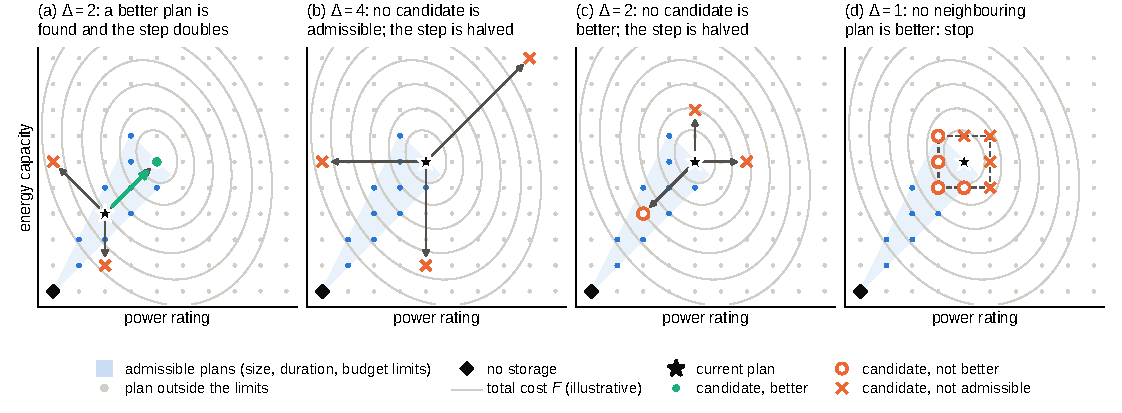
\includegraphics[width=1.00\textwidth]{fig_search_generic.pdf}
%DIF >     \caption{Illustration of the discrete planning search in two dimensions. Shading identifies admissible plans; contours show an illustrative objective unavailable to the search. (a) An improving candidate is accepted and the poll size increases. (b--c) Unsuccessful polls reduce the poll size. (d) A completed unit poll finds no improvement beyond the acceptance threshold, and the search terminates.}
%DIF >     \label{fig:search_generic}
%DIF > \end{figure}

 
    \DIFadd{Candidate plans are generated by a granular MADS-based search~\mbox{%DIFAUXCMD
\cite{audet_dennis_2006,audet_granular_2019}}\hskip0pt%DIFAUXCMD
, summarised in Algorithm~\ref{alg:shared_ess_planning_mads}.
    For each interface node, the search selects converter rating and energy capacity in discrete increments, together with one installation year common to all selected nodes.
    The general formulation permits independent installation years and staged additions, which are not explored in the case study.
}


\begin{algorithm}[htbp!]
    \caption{Derivative-free shared-ESS planning search.}
    \label{alg:shared_ess_planning_mads}
    \DontPrintSemicolon
    \KwIn{Lattice and admissibility conditions \eqref{eq:master_rated_s}--\eqref{eq:master_budget}; $\Delta_0$, $N^{\max}$, $\sigma_Q$; poll variant; cache $\mathcal{C}$.}
    \KwOut{Incumbent plan $\boldsymbol{x}^{\star}$ and the scope of its final unit poll.}
    $\boldsymbol{z} \in \mathbb{Z}^{2|E^S|+1}$: the lattice coordinates of $\boldsymbol{x}$ and the investment year; admissibility checked in closed form\;
    $\boldsymbol{x}^{\text{inc}} \gets \arg\min F$ over the certified, budget-feasible points of $\mathcal{C}$ ($\boldsymbol{x} = \boldsymbol{0}$ included; ties to the lower investment); $\Delta \gets \Delta_0$; $N \gets 0$\;
    \While{polls remain and a poll can be launched}{
        \uIf{variant A}{
            $\mathcal{P} \gets$ the $n+1$ OrthoMADS points $\boldsymbol{z}^{\text{inc}} + \Delta \boldsymbol{v}$, inadmissible ones dropped; \lIf{$\Delta = 1$}{$\mathcal{P} \gets \mathcal{P} \cup$ every admissible unit neighbour of $\boldsymbol{z}^{\text{inc}}$ ($\infty$-norm box)}
        }
        \Else(variant B, $\Delta = 1$ throughout){
            $\mathcal{P} \gets$ the $2n$ OrthoMADS points $\boldsymbol{z}^{\text{inc}} \pm \boldsymbol{v}$, each inadmissible point snapped to the nearest admissible point of the unit frame; \lIf{fewer than $n+1$ distinct points}{add every admissible unit neighbour}
        }
        \lIf{$|\mathcal{P}|$ exceeds the completion cap, or the new points of $\mathcal{P}$ exceed $N^{\max} - N$}{\textbf{stop}}
        Evaluate each new point of $\mathcal{P}$ by Algorithm~\ref{alg:operational_planning_degradation} under its production exit; record $F$, its settling bar and its exit (a failed evaluation is a barrier point, $F = +\infty$); add the records to $\mathcal{C}$; $N \gets N +$ new evaluations\;
        \eIf{some $\boldsymbol{x} \in \mathcal{P}$ has $F(\boldsymbol{x}^{\text{inc}}) - F(\boldsymbol{x}) > \max\{\text{bar}_{\boldsymbol{x}} + \text{bar}_{\text{inc}},\, \sigma_Q\}$}{
            $\boldsymbol{x}^{\text{inc}} \gets$ the best such point; $\Delta \gets 2\Delta$ (variant A) or $1$ (variant B)\;
        }{
            \lIf{$\Delta = 1$}{\textbf{terminate}: no evaluated unit neighbour improves $\boldsymbol{x}^{\text{inc}}$}
            $\Delta \gets \Delta/2$\;
        }
    }
    \Return{$\boldsymbol{x}^{\text{inc}}$, the poll history and the scope of the final unit poll}\;
\end{algorithm}


    \DIFadd{At each iteration, candidate plans are generated around the incumbent using OrthoMADS directions~\mbox{%DIFAUXCMD
\cite{abramson_orthomads_2009}}\hskip0pt%DIFAUXCMD
.
    Their operating costs are evaluated using the production stopping rule. A candidate is accepted only when its improvement exceeds the numerical acceptance threshold in Algorithm~\ref{alg:shared_ess_planning_mads}. The settling bar is the largest absolute objective change over an evaluation's final ten cycles. The search threshold is a cheap screen on the production stopping rule; the comparisons reported in Section~\ref{sec:results} are re-evaluated under the acceptance criteria of Subsection~\ref{subsubsec:certification}, whose threshold is stated there.
}



    \DIFadd{In variant A, the poll size increases after success and decreases after failure; variant B maintains a unit poll size.
    Variant A evaluates every admissible unit neighbour before declaring a unit poll unsuccessful. Search termination therefore establishes only the outcome of }\DIFaddend the \DIFdelbegin \DIFdel{TSO and DSO subproblems across representative years while maintaining intertemporal consistency of ESS degradation over the planning horizon. }\DIFdelend \DIFaddbegin \DIFadd{evaluated neighbourhood; it does not establish global optimality. Search limits and parameter values are specified in \ref{app:results_statistics}.
}\DIFaddend 


\subsection{Master Problem}
\DIFaddbegin \label{subsec:master}
\DIFaddend 

At the master\DIFaddbegin \DIFadd{-planning}\DIFaddend  level, the framework determines \DIFdelbegin \DIFdel{strategic investment decisions }\DIFdelend \DIFaddbegin \DIFadd{a single, scenario-independent multi-year investment plan }\DIFaddend for shared ESSs at \DIFdelbegin \DIFdel{TN--DN }\DIFdelend \DIFaddbegin \DIFadd{TN–DN }\DIFaddend interface nodes, including siting, sizing, and staged capacity expansion\DIFdelbegin \DIFdel{over the planning horizon. Investment-cost uncertainty }\DIFdelend \DIFaddbegin \DIFadd{. Uncertainty in future ESS investment costs }\DIFaddend is represented through a set of \DIFaddbegin \DIFadd{low, medium, and high }\DIFaddend cost trajectories. \DIFdelbegin \DIFdel{The master problem evaluates investment decisions under these trajectories and computes the corresponding scenario-weighted expected investment levels used in the lower-level operational evaluation}\DIFdelend \DIFaddbegin \DIFadd{These trajectories affect the expected investment expenditure, but the physical investment decisions remain common to all scenarios and are passed directly to the operational recourse problem}\DIFaddend .
%Under this modeling choice, the operational subproblem assesses the expected shared ESS deployment induced by the investment-cost uncertainty representation. This approximation preserves tractability while allowing the planning layer to internalize uncertain investment conditions.

\subsubsection{Objective Function}

The \DIFdelbegin \DIFdel{master problem minimizes }\DIFdelend \DIFaddbegin \DIFadd{planning search seeks to minimise }\DIFaddend the expected discounted investment cost \DIFdelbegin \DIFdel{of shared ESSs, expressed as}\DIFdelend \DIFaddbegin \DIFadd{plus the evaluated expected discounted operating cost of the investment plan}\DIFaddend :


    \DIFdelbegin \begin{displaymath}
    \DIFdel{\min \sum_{e \in E^S} \sum_{y \in Y} \sum_{c \in \Omega_C} 
    \Bigg( 
        \frac{\omega_c}{(1 + r)^{y - y_0}} 
        \left( 
            c^{\text{Inv,S}}_{y,c} S^{\text{Inv}(l)}_{e,y,c} + 
            c^{\text{Inv,E}}_{y,c} E^{\text{Inv}(l)}_{e,y,c} 
        \right)
    \Bigg)
    + \alpha^{(l)}
}\end{displaymath}%DIFAUXCMD
\DIFdelend \DIFaddbegin \begin{equation}
        \DIFadd{\min_{\boldsymbol{x}\in\mathcal{X}} F(\boldsymbol{x})
        \label{eq:master_objective}
    }\end{equation}\DIFaddend 



    \DIFaddbegin \begin{equation}
        \DIFadd{F(\boldsymbol{x}) = I(\boldsymbol{x}) + Q(\boldsymbol{x})
        \label{eq:master_objective_value}
    }\end{equation}



    \DIFadd{The expected discounted investment cost is given by:
}



    \begin{equation}
        \DIFadd{I(\boldsymbol{x}) = \sum_{e\in E^S} \sum_{y^{\text{Inv}}\in Y} \sum_{c\in\Omega_C} \frac{\omega_c}{(1+r)^{y^{\text{Inv}}-y_0}}
        \left(
            c^{\text{Inv,S}}_{y^{\text{Inv}},c} S^{\text{Inv}}_{e,y^{\text{Inv}}}
            +
            c^{\text{Inv,E}}_{y^{\text{Inv}},c} E^{\text{Inv}}_{e,y^{\text{Inv}}}
        \right)
    }\end{equation}


\DIFaddend \noindent
\DIFdelbegin \DIFdel{where 
$c^{\text{Inv,S}}_{y,c}$ and $c^{\text{Inv,E}}_{y,c}$ denote the scenario-dependent unit investment }\DIFdelend \DIFaddbegin 

    \DIFadd{where $c^{\text{Inv,S}}_{y^{\text{Inv}},c}$ and $c^{\text{Inv,E}}_{y^{\text{Inv}},c}$ are the unit }\DIFaddend costs of converter \DIFaddbegin \DIFadd{apparent-}\DIFaddend power rating and energy capacity \DIFdelbegin \DIFdel{, respectively; 
$S^{\text{Inv}(l)}_{e,y,c}$ and $E^{\text{Inv}(l)}_{e,y,c}$ are the corresponding investment decisions; and 
$\alpha^{(l)}$ is an auxiliary variable representing the Benders underestimator of the operational cost term}\DIFdelend \DIFaddbegin \DIFadd{in installation year $y^{\text{Inv}}$ under cost trajectory $c$.
    The variables $S^{\text{Inv}}_{e,y^{\text{Inv}}}$ and $E^{\text{Inv}}_{e,y^{\text{Inv}}}$ denote the corresponding capacity additions at node $e$. Investment expenditure is weighted by the trajectory probabilities $\omega_c$ and discounted to the initial year $y_0$ at rate $r$}\DIFaddend .



    \DIFaddbegin \DIFadd{The investment decisions are common to all cost trajectories: uncertainty affects the expected expenditure, rather than producing scenario-dependent physical capacities.
    The term $Q(\boldsymbol{x})$ is the expected discounted operating cost returned by the operational evaluation, as defined in Subsection~\ref{subsubsec:certification}.
}


\DIFaddend \subsubsection{Total Rated Power and Energy Capacity}


    \DIFdelbegin \DIFdel{The }\textit{\DIFdel{total}} %DIFAUXCMD
\DIFdel{rated }\DIFdelend \DIFaddbegin \DIFadd{For each node $e$ and representative year $y$, the set of
    installation years whose cohorts remain active is:
    }\begin{equation}
        \DIFadd{\mathcal{Y}^{\text{Act}}_{e,y}
        =
        \left\{
            y^{\text{Inv}}\in Y :
            y^{\text{Inv}}\le y,\quad
            y-y^{\text{Inv}}<
            T^{\text{Cal}}_{e,y^{\text{Inv}}}
        \right\}.
        \label{eq:active_cohorts}
    }\end{equation}
    \DIFadd{An installation contributes only after it has been made
    and before its calendar lifetime expires.
}



    \DIFadd{The total rated converter apparent }\DIFaddend power and energy capacity \DIFdelbegin \DIFdel{of each shared ESS are cumulative functions of the yearly investments made throughout the planning horizon and are limited by the calendar lifetime of each installation ($\forall e \in E^S$, $\forall y \in Y$, $\forall c \in \Omega_C$, $\forall l \in L^B$}\DIFdelend \DIFaddbegin \DIFadd{at node $e$ in representative year $y$ are obtained by summing the capacity additions whose calendar lifetimes have not expired ($\forall e\in E^S$, $\forall y\in Y$}\DIFaddend ):



    \DIFdelbegin \begin{displaymath}
    \DIFdel{S^{\text{Rated}(l)}_{e,y,c} = \sum_{y^\text{Inv}=\max(y-T^\text{Cal}_{e,y},\,y_0)}^{y} S^{\text{Inv}(l)}_{e,y^\text{Inv},c}
}\end{displaymath}%DIFAUXCMD
\DIFdelend \DIFaddbegin \begin{equation}
        \DIFadd{S^{\text{Rated}}_{e,y}
        =
        \sum_{y^{\text{Inv}}\in\mathcal{Y}^{\text{Act}}_{e,y}}
        S^{\text{Inv}}_{e,y^{\text{Inv}}}
        \label{eq:master_rated_s}
    }\end{equation}\DIFaddend 



    \DIFdelbegin \begin{displaymath}
    \DIFdel{E^{\text{Rated}(l)}_{e,y,c} = \sum_{y^\text{Inv}=\max(y-T^\text{Cal}_{e,y},\,y_0)}^{y} E^{\text{Inv}(l)}_{e,y^\text{Inv},c}
}\end{displaymath}%DIFAUXCMD
\DIFdelend \DIFaddbegin \begin{equation}
        \DIFadd{E^{\text{Rated}}_{e,y}
        =
        \sum_{y^{\text{Inv}}\in\mathcal{Y}^{\text{Act}}_{e,y}}
        E^{\text{Inv}}_{e,y^{\text{Inv}}}
    }\end{equation}\DIFaddend 


\noindent
\DIFdelbegin \DIFdel{where 
$S^{\text{Rated}(l)}_{e,y,c}$ and $E^{\text{Rated}(l)}_{e,y,c}$ denote the total rated power }\DIFdelend \DIFaddbegin 

    \DIFadd{where 
    $S^{\text{Inv}}_{e,y^{\text{Inv}}}$ and $E^{\text{Inv}}_{e,y^{\text{Inv}}}$ denote the converter apparent-power rating }\DIFaddend and energy capacity \DIFdelbegin \DIFdel{available }\DIFdelend \DIFaddbegin \DIFadd{installed }\DIFaddend at node $e$ in year \DIFdelbegin \DIFdel{$y$, under investment scenario $c$, at iteration $l$; 
$S^{\text{Inv}(l)}_{e,y^\text{Inv},c}$ and
    $E^{\text{Inv}(l)}_{e,y^\text{Inv},c}$ denote the corresponding incremental investments in rated power and energy capacity made in year $y^\text{Inv}$; and 
$T^\text{Cal}_{e,y}$ }\DIFdelend \DIFaddbegin \DIFadd{$y^{\text{Inv}}$, and
    $T^{\text{Cal}}_{e,y^{\text{Inv}}}$ }\DIFaddend is the calendar lifetime of \DIFdelbegin \DIFdel{ESS $e$, installed in year $y$}\DIFdelend \DIFaddbegin \DIFadd{that installation. 
    Rated capacities represent installed nameplate capacities; the reduction in available energy due to degradation is accounted for in the operational subproblem}\DIFaddend .



    \DIFaddbegin \DIFadd{Capacity additions are restricted to non-negative integer multiples of $\Delta^S$ and $\Delta^E$, respectively, defining the discrete investment space.
}


\DIFaddend \subsubsection{Maximum Installable Capacity}

\DIFdelbegin \DIFdel{Each shared ESS is subject to an upper bound on installable energy }\DIFdelend \DIFaddbegin \DIFadd{The total rated energy capacity at each interface node is bounded by the maximum installable }\DIFaddend capacity, reflecting physical, spatial \DIFdelbegin \DIFdel{, }\DIFdelend or technical constraints at the \DIFdelbegin \DIFdel{corresponding TN--DN interface substation ($\forall e \in E^S$, $\forall y \in Y$, $\forall c \in \Omega_C$, $\forall l \in L^B$}\DIFdelend \DIFaddbegin \DIFadd{substation ($\forall e\in E^S$, $\forall y\in Y$}\DIFaddend ):

\DIFdelbegin \begin{displaymath}
    \DIFdel{E_{e,y,c}^{\text{Rated}(l)} \leq E^{\text{Max}}_{e,y}
}\end{displaymath}%DIFAUXCMD
\DIFdelend \DIFaddbegin \begin{equation}
    \DIFadd{E_{e,y}^{\text{Rated}} \leq E^{\text{Max}}_{e,y}
}\end{equation}\DIFaddend 

\noindent
\DIFaddbegin 

    \DIFaddend where $E^{\text{Max}}_{e,y}$ \DIFdelbegin \DIFdel{denotes the maximum installable capacity for ESS }\DIFdelend \DIFaddbegin \DIFadd{is the maximum total rated energy capacity permitted at node }\DIFaddend $e$ in \DIFaddbegin \DIFadd{representative }\DIFaddend year $y$.


\subsubsection{\DIFdelbegin \DIFdel{Energy-to-Power Capacity }\DIFdelend \DIFaddbegin \DIFadd{Energy-to-Converter-Rating }\DIFaddend Ratio}


    \DIFdelbegin \DIFdel{Battery-based ESSs are characterized by technology- and application-specific energy-to-power ratios, enforced through the following constraint ($\forall e \in E^S$, $\forall y \in Y$, $\forall c \in \Omega_C$, $\forall l \in L^B$}\DIFdelend \DIFaddbegin \DIFadd{Each capacity addition is subject to bounds on the ratio of rated energy capacity to converter apparent-power rating ($\forall e\in E^S$, $\forall y^{\text{Inv}}\in Y$}\DIFaddend ):



    \DIFdelbegin \begin{displaymath}
    \DIFdel{\phi^{\text{Min}}_e S^{\text{Inv}(l)}_{e,y,c} \leq 
    E^{\text{Inv}(l)}_{e,y,c} \leq 
    \phi^{\text{Max}}_e S^{\text{Inv}(l)}_{e,y,c}
}\end{displaymath}%DIFAUXCMD
\DIFdelend \DIFaddbegin \begin{equation}
        \DIFadd{\phi^{\text{Min}}_e S^{\text{Inv}}_{e,y^{\text{Inv}}} \leq 
        E^{\text{Inv}}_{e,y^{\text{Inv}}} \leq 
        \phi^{\text{Max}}_e S^{\text{Inv}}_{e,y^{\text{Inv}}}
        \label{eq:master_duration}
    }\end{equation}\DIFaddend 


\noindent
\DIFaddbegin 

    \DIFaddend where $\phi^{\text{Min}}_e$ and $\phi^{\text{Max}}_e$ \DIFdelbegin \DIFdel{denote }\DIFdelend \DIFaddbegin \DIFadd{are }\DIFaddend the minimum and maximum admissible \DIFdelbegin \DIFdel{energy-to-power ratiosfor shared ESS $e$}\DIFdelend \DIFaddbegin \DIFadd{energy-to-converter-rating ratios, expressed in MWh/MVA}\DIFaddend . These bounds constrain \DIFdelbegin \DIFdel{storage duration according to the selected technology and use case.
Typical values for utility-scale lithium-ion batteries range from 2~h to 10~h~\mbox{%DIFAUXCMD
\cite{nrel_ess_costs}}\hskip0pt%DIFAUXCMD
. }\DIFdelend \DIFaddbegin \DIFadd{the relative sizing of the battery and converter.
}\DIFaddend 



    \DIFaddbegin \DIFadd{At unity power factor, the converter's apparent-power rating corresponds numerically to its maximum active-power output. The ratio is therefore used as a nominal duration indicator. It does not represent the achievable discharge duration, which also depends on usable energy, discharge efficiency, degradation and reactive-power provision.
}


\DIFaddend \subsubsection{\DIFdelbegin \DIFdel{Available Budget}\DIFdelend \DIFaddbegin \DIFadd{Expected Discounted Investment-Expenditure Limit}\DIFaddend }


    The \DIFdelbegin \DIFdel{total discounted investment cost incurred over the planning horizon is constrained by the available budget($\forall l \in L^B$)}\DIFdelend \DIFaddbegin \DIFadd{expected discounted expenditure of the investment plan is bounded by the planning budget}\DIFaddend :


\DIFdelbegin \begin{displaymath}
    \DIFdel{\sum_{e \in E^S} \sum_{y \in Y} \sum_{c \in \Omega_C} 
    \frac{\omega_c}{(1 + r)^{y - y_0}}
    \left(
        c^{\text{Inv,S}}_{y,c} S^{\text{Inv}(l)}_{e,y,c}
        + 
        c^{\text{Inv,E}}_{y,c} E^{\text{Inv}(l)}_{e,y,c}
    \right)
    \leq c^{\text{Inv}}
}\end{displaymath}%DIFAUXCMD
\DIFdelend \DIFaddbegin \begin{equation}
    \DIFadd{I(\boldsymbol{x}) \leq c^{\text{Inv}}
    \label{eq:master_budget}
}\end{equation}\DIFaddend 

\noindent
\DIFaddbegin 

    \DIFaddend where 
    $c^{\text{Inv}}$ \DIFdelbegin \DIFdel{denotes the total investment budget allocated to shared ESSs.
    }%DIFDELCMD < 

%DIFDELCMD < %%%
\subsubsection{\DIFdel{Expected Rated Power and Energy Capacity}}
%DIFAUXCMD
\addtocounter{subsubsection}{-1}%DIFAUXCMD
%DIFDELCMD < 

%DIFDELCMD < %%%
\DIFdel{The }\textit{\DIFdel{expected}} %DIFAUXCMD
\DIFdel{rated power and energy capacities are defined as }\DIFdelend \DIFaddbegin \DIFadd{is the budget for expected investment expenditure discounted to the initial year $y_0$.
    The constraint applies to the }\DIFaddend probability-weighted \DIFdelbegin \DIFdel{averages over all }\DIFdelend \DIFaddbegin \DIFadd{expenditure over the }\DIFaddend investment-cost \DIFdelbegin \DIFdel{scenarios $c \in \Omega_C$ ($\forall e \in E^S$, $\forall y \in Y$, $\forall l \in L^B$):
}\DIFdelend \DIFaddbegin \DIFadd{trajectories. It does not require expenditure under every individual trajectory to remain within the budget.
}\DIFaddend 



    \DIFdelbegin \begin{displaymath}
    \DIFdel{S^{\text{Rated}(l)}_{e,y} = \sum_{c \in \Omega_C} \omega_c \, S^{\text{Rated}(l)}_{e,y,c}
}\end{displaymath}%DIFAUXCMD
%DIFDELCMD < 

%DIFDELCMD < %%%
\begin{displaymath}
    \DIFdel{E^{\text{Rated}(l)}_{e,y} = \sum_{c \in \Omega_C} \omega_c \, E^{\text{Rated}(l)}_{e,y,c}
}\end{displaymath}%DIFAUXCMD
%DIFDELCMD < 

%DIFDELCMD < %%%
\DIFdel{Analogously, the expected investment decisions for rated power and energy capacity are given by ($\forall e \in E^S$, $\forall y \in Y$, $\forall l \in L^B$):
}%DIFDELCMD < 

%DIFDELCMD < %%%
\begin{displaymath}
    \DIFdel{S^{\text{Inv}(l)}_{e,y} = \sum_{c \in \Omega_C} \omega_c \, S^{\text{Inv}(l)}_{e,y,c}
}\end{displaymath}%DIFAUXCMD
%DIFDELCMD < 

%DIFDELCMD < %%%
\begin{displaymath}
    \DIFdel{E^{\text{Inv}(l)}_{e,y} = \sum_{c \in \Omega_C} \omega_c \, E^{\text{Inv}(l)}_{e,y,c}
}\end{displaymath}%DIFAUXCMD
%DIFDELCMD < 

%DIFDELCMD < %%%
\DIFdel{These expected investment variables form the coupling variables between the master and operational problems. At each iteration $l \in L^B$, the master problem computes a scenario-aggregated investment plan, which is then passed to the subproblem for coordinated multi-year TSO--DSO operational evaluation}\DIFdelend \DIFaddbegin \DIFadd{Together, \eqref{eq:master_rated_s}--\eqref{eq:master_budget} and the integrality of the investments define the admissible set $\mathcal{X}$, a finite set of discrete plans}\DIFaddend . 


%DIF < In the present formulation, investment-cost uncertainty is represented through scenario-dependent cost coefficients and the corresponding scenario-weighted investment quantities. The operational subproblem is then evaluated using the expected investment plan, which acts as a scenario-aggregated representation of the installed shared ESS capacity. This modeling choice yields a risk-neutral planning approximation that preserves tractability of the bi-level decomposition. Accordingly, the framework should be interpreted as determining an expected long-term shared ESS expansion plan under uncertain investment trajectories, rather than as a fully multi-stage stochastic program with explicit non-anticipativity constraints.
%DIF > \subsubsection{Coupling Between Planning and Operational Recourse}

\DIFdelbegin \subsubsection{\DIFdel{Benders' Cuts}}
%DIFAUXCMD
\addtocounter{subsubsection}{-1}%DIFAUXCMD
\DIFdelend %DIF > 
%DIF >     For each candidate plan, the scenario-independent capacity additions $S^{\text{Inv}}_{e,y^{\text{Inv}}}$ and $E^{\text{Inv}}_{e,y^{\text{Inv}}}$ are held fixed in the operational subproblem, where they enter as the parameters $\hat{S}^{\text{Inv}}_{e,y^{\text{Inv}}}$ and $\hat{E}^{\text{Inv}}_{e,y^{\text{Inv}}}$ of Subsection~\ref{subsubsec:capacity}. The resulting evaluated operating cost $Q(\boldsymbol{x})$, together with its stopping status and numerical diagnostics, is returned to the planning search. The evaluation and numerical acceptance criteria are described in Subsection~\ref{subsubsec:certification}.
%DIF > 

\DIFdelbegin \DIFdel{The Benders' decomposition procedure iteratively refines the master problem by adding cuts derived from the operational evaluation of candidate investment plans. When the operational subproblem is feasible, an optimality cut is generated from the corresponding sensitivities with respect to the coupling variables ($\forall k = 1, \ldots, l-1$)}\DIFdelend \DIFaddbegin \subsubsection{\DIFadd{Recourse Evaluation and Numerical Acceptance}}
\label{subsubsec:certification}


    \DIFadd{The evaluated expected discounted operating cost of a fixed investment plan is obtained by aggregating the daily costs returned by the TSO--DSO coordination procedure}\DIFaddend :



    \DIFdelbegin \begin{displaymath}
    \DIFdel{\alpha^{(l)} \ge y^{(k)} 
    +
    \sum_{e \in E^S}\sum_{y \in Y}
    \mu^{S(k)}_{e,y}\left(S^{\text{Inv}(l)}_{e,y}-S^{\text{Inv}(k)}_{e,y}\right)
    +
    \sum_{e \in E^S}\sum_{y \in Y}
    \mu^{E(k)}_{e,y}\left(E^{\text{Inv}(l)}_{e,y}-E^{\text{Inv}(k)}_{e,y}\right)
}\end{displaymath}%DIFAUXCMD
\DIFdelend \DIFaddbegin \begin{equation}
        \DIFadd{Q(\boldsymbol{x}) =
        \sum_{y \in Y} \frac{Y_y}{(1+r)^{y-y_0}}
        \sum_{d \in D} D_d
        \sum_{m \in \Omega_M} \sum_{o \in \Omega_O} \omega_m \, \omega_o \,
        C^{\text{Op}}_{y,d,m,o}(\boldsymbol{x})
        \label{eq:recourse_value}
    }\end{equation}\DIFaddend 


\noindent
\DIFdelbegin \DIFdel{where 
$y^{(k)}$ denotes the subproblem objective value at iteration $k$, and 
$\mu^{S(k)}_{e,y}$ and $\mu^{E(k)}_{e,y}$ are the corresponding sensitivity coefficients associated with the power and energy investment variables. }%DIFDELCMD < 

%DIFDELCMD < %%%
\DIFdel{To preserve subproblem feasibility, the shared ESS subproblem }\DIFdelend \DIFaddbegin 

    \DIFadd{where 
    $C^{\text{Op}}_{y,d,m,o}(\boldsymbol{x})$ is the evaluated daily operating cost for representative year $y$, day $d$, market scenario $m$ and operation scenario $o$. It includes TN generation costs, activated DN flexibility, and penalties on storage energy-closure and network-feasibility slacks. In the multi-scenario instance, it also includes the commitment charge and the deviation component of interface settlement }\DIFaddend (Subsection~\DIFdelbegin \DIFdel{\ref{subsec:subproblem})includes penalized slack variables.
Their activation indicates that the corresponding investment plan is not operationally feasible without relaxing the operational constraints. The associated sensitivity information is then used to discourage similar investment solutions in subsequent iterations ($\forall k = 1, \ldots, l-1$):
}\DIFdelend \DIFaddbegin \DIFadd{\ref{subsubsec:commitment}).
}\DIFaddend 



    \DIFdelbegin \begin{displaymath}
    \DIFdel{0 \geq -y^{(k)} 
    + 
    \sum_{e \in E^S}\sum_{y \in Y}
    \mu^{S(k)}_{e,y} \left( S^{\text{Inv}(l)}_{e,y} - S^{\text{Inv}(k)}_{e,y} \right) 
    + 
    \sum_{e \in E^S}\sum_{y \in Y}
    \mu^{E(k)}_{e,y} \left( E^{\text{Inv}(l)}_{e,y} - E^{\text{Inv}(k)}_{e,y} \right)
}\end{displaymath}%DIFAUXCMD
\DIFdelend \DIFaddbegin \DIFadd{The contracted component of interface settlement is excluded as a transfer between operators. Storage-agent and solver regularisation terms are also excluded. Renewable curtailment is assigned no cost and is reported separately as curtailed energy.
}\DIFaddend 



    \DIFdelbegin \DIFdel{Finally, to prevent numerical instability during the initial iterations, the underestimator is bounded from below as :
}\DIFdelend \DIFaddbegin \DIFadd{The weights $Y_y$ and $D_d$ are the numbers of calendar years and days represented by $y$ and $d$, respectively. Operating costs are discounted to $y_0$ at the representative year $y$ of each block rather than year by year within the block, an approximation common to every evaluated plan.
}\DIFaddend 



    \DIFdelbegin \begin{displaymath}
    \DIFdel{\alpha^{(l)} \geq \alpha^{\text{Down}}
}\end{displaymath}%DIFAUXCMD
\DIFdelend \DIFaddbegin \DIFadd{Search evaluations and the multi-scenario evaluations use the residual-based production stopping rule. 
    For the single-scenario comparisons, additional numerical acceptance criteria assess objective stability, the priced interface-consensus gap and the quality of the local solves.
    Evaluations that satisfy these criteria are termed certified; those that do not satisfy them within the iteration limit are reported as uncertified. 
    The complete procedure is specified in \ref{app:admm_updated_certification}.
}\DIFaddend 



    \DIFdelbegin %DIFDELCMD < \noindent
%DIFDELCMD < %%%
\DIFdelend \DIFaddbegin \DIFadd{A difference between two certified evaluations is classified as determinate when its magnitude is at least $\max\{3b,2\tau\}$, }\DIFaddend where \DIFdelbegin \DIFdel{$\alpha^{\text{Down}}$ is a predefined lower bound ensuring numerical stability.
}%DIFDELCMD < 

%DIFDELCMD < %%%
\subsection{\DIFdel{Subproblem}}
%DIFAUXCMD
\addtocounter{subsection}{-1}%DIFAUXCMD
%DIFDELCMD < \label{subsec:subproblem}
%DIFDELCMD < 

%DIFDELCMD < %%%
\DIFdel{The operational subproblem is decomposed into one TSO subproblem, a set of DSO subproblems, and a dedicated shared ESS subproblem. 
    For scalability, }\DIFdelend \DIFaddbegin \DIFadd{$b$ is the larger objective range over their acceptance windows and $\tau$ is }\DIFaddend the \DIFdelbegin \DIFdel{formulation is further decomposed across representative years and representative days.
    In this formulation, inter-year coupling arises exclusively from ESS degradation and is enforced through the shared ESS subproblem. This structure preserves tractability, scalability, data privacy, and regulatory compliance, since each SO relies only on local proprietary information. }\DIFdelend \DIFaddbegin \DIFadd{prescribed objective tolerance. Differences involving uncertified evaluations are assessed using the consensus-gap and objective-settling criteria specified in \ref{app:admm_updated_certification}. Differences below the applicable threshold are reported as within numerical resolution.
}\DIFaddend 



    \DIFdelbegin \subsubsection{\DIFdel{Shared ESS Operation Subproblem}}
%DIFAUXCMD
\addtocounter{subsubsection}{-1}%DIFAUXCMD
%DIFDELCMD < 

%DIFDELCMD < %%%
\DIFdel{To capture the intertemporal effects of battery degradation, the ADMM-based coordination framework introduced in~\mbox{%DIFAUXCMD
\cite{simoes_2023} }\hskip0pt%DIFAUXCMD
is extended with an additional agent representing the shared ESS subproblem. This agent links short-term operating decisions with long-term degradation dynamics by tracking the evolution of State-of-Health (SoH)and available energy capacity across representative years.
    Algorithm~\ref{alg:operational_planning_degradation}, }\DIFdelend \DIFaddbegin \DIFadd{These criteria assess the numerical stability of the returned operating costs. A certified evaluation is an approximate first-order stationary point of the coupled recourse that is AC-feasible within the consensus tolerances (\ref{app:admm_updated_certification}); it carries no global guarantee.
    Parameter values are }\DIFaddend given in~\DIFdelbegin \DIFdel{\ref{app:admm_updated_algorithm}, presents the updated pseudo-code of the coordination procedure, while~\ref{app:admm_updated_implementation} details the corresponding mathematical formulation}\DIFdelend \DIFaddbegin \DIFadd{\ref{app:results_statistics}, and the single-scenario evaluation records are provided in~\ref{app:results}}\DIFaddend .


\DIFdelbegin \subsubsection{\DIFdel{Shared ESS Mathematical Formulation}}
%DIFAUXCMD
\addtocounter{subsubsection}{-1}%DIFAUXCMD
\DIFdelend \DIFaddbegin \subsection{\DIFadd{Operational Subproblem}}
\label{subsec:subproblem}
\DIFaddend 


    \DIFdelbegin \DIFdel{Investment decisions on rated power and energy capacity determined by the master problem are treated as fixed parameters in the subproblem. These decisions are enforced through }\DIFdelend \DIFaddbegin \DIFadd{For a fixed investment plan, coordinated operation comprises TSO and DSO network models for each representative year--day pair and one shared-ESS agent per interface node spanning all representative years and days. The network models enforce stored-energy dynamics and converter limits, while the shared-ESS agents track degradation and available energy capacity. The models are coupled through ADMM consensus on the net active- and reactive-power schedules.
    Degradation is calculated from the charging and discharging variables of the shared-ESS agents.
}



    \DIFadd{Each network block includes all market and operation scenarios, weighted by their probabilities. The shared-ESS schedule and the TSO's interface exchange are common to these scenarios; the shared-ESS agents therefore carry no scenario index. Scenario indices are omitted from the storage equations below.
}



    \DIFadd{The local coordination problems are specified in \ref{app:admm_updated_implementation}, and }\DIFaddend the \DIFdelbegin \DIFdel{following constraints ($\forall e \in E^S$, $\forall y \in Y$):
}\DIFdelend \DIFaddbegin \DIFadd{solution procedure is summarised in Algorithm~\ref{alg:operational_planning_degradation}.
}\DIFaddend 


\DIFdelbegin \begin{displaymath}
    \DIFdel{S^{\text{Inv}}_{e,y} = \hat{S}^{\text{Inv}}_{e,y} + S^{\text{Up}}_{e,y} - S^{\text{Down}}_{e,y}
}\end{displaymath}%DIFAUXCMD
\DIFdelend \DIFaddbegin \subsubsection{\DIFadd{Installed and Available Capacity}}
\label{subsubsec:capacity}


    \DIFadd{Each capacity addition defines a cohort identified by its node $e$ and installation year $y^{\text{Inv}}$.
    For active cohorts, rated capacities equal the fixed investment values specified by the candidate plan ($\forall e\in E^S$, $\forall y\in Y$, $\forall y^{\text{Inv}}\in\mathcal{Y}^{\text{Act}}_{e,y}$):
}



    \begin{equation}
        \DIFadd{S^{\text{Rated,Unit}}_{e,y^\text{Inv},y} = \hat{S}^{\text{Inv}}_{e,y^\text{Inv}}
        \label{eq:cohort_rated}
    }\end{equation}\DIFaddend 



    \DIFdelbegin \begin{displaymath}
    \DIFdel{E^{\text{Inv}}_{e,y} = \hat{E}^{\text{Inv}}_{e,y} + E^{\text{Up}}_{e,y} - E^{\text{Down}}_{e,y}
}\end{displaymath}%DIFAUXCMD
\DIFdelend \DIFaddbegin \begin{equation}
        \DIFadd{E^{\text{Rated,Unit}}_{e,y^\text{Inv},y} = \hat{E}^{\text{Inv}}_{e,y^\text{Inv}}
        \label{eq:cohort_rated_energy}
    }\end{equation}\DIFaddend 



    \DIFdelbegin %DIFDELCMD < \noindent
%DIFDELCMD < %%%
\DIFdel{where 
$\hat{S}^{\text{Inv}}_{e,y}$ and $\hat{E}^{\text{Inv}}_{e,y}$ denote the expected investments in power rating and energy capacity, respectively, for ESS $e$ in year $y$. The variables $S^{\text{Up}}_{e,y}$, $S^{\text{Down}}_{e,y}$, $E^{\text{Up}}_{e,y}$, and $E^{\text{Down}}_{e,y}$ are slack variables introduced to preserve subproblem feasibility under all operating conditions. These slack variables are penalized in the subproblem objective function to discourage deviations from the investment targets determined at the master level.
}\DIFdelend \DIFaddbegin \DIFadd{The converter rating remains unchanged by degradation. Available energy is evaluated using end-of-block state of health, giving a conservative within-block capacity estimate:
}\DIFaddend 



    \DIFdelbegin \DIFdel{The rated power and energy capacity of each shared ESS over the planning horizon are determined by investments made in successive representative years.
To explicitly capture this evolution, auxiliary variables are introduced to represent the contribution of each investment throughout its operational lifetime ($\forall e \in E^S$, $\forall y^\text{Inv} \in Y$, }\DIFdelend \DIFaddbegin \begin{equation}
        \DIFadd{S^{\text{Av,Unit}}_{e,y^\text{Inv},y} = S^{\text{Rated,Unit}}_{e,y^\text{Inv},y}
        \label{eq:cohort_available}
    }\end{equation}



    \begin{equation}
        \DIFadd{E^{\text{Av,Unit}}_{e,y^\text{Inv},y} = E^{\text{Rated,Unit}}_{e,y^\text{Inv},y}\, SoH_{e,y^\text{Inv},y}
        \label{eq:cohort_available_energy}
    }\end{equation}



    \DIFadd{At each coordination cycle, the shared-ESS agent supplies the network models with the total available capacities, obtained by summing over active cohorts ($\forall e\in E^S$, $\forall y\in Y$):
}



    \begin{equation}
        \DIFadd{S^{\text{Av}}_{e,y} = \sum_{y^{\text{Inv}}\in\mathcal{Y}^{\text{Act}}_{e,y}} S^{\text{Av,Unit}}_{e,y^{\text{Inv}},y}
        \label{eq:available_power}
    }\end{equation}



    \begin{equation}
        \DIFadd{E^{\text{Av}}_{e,y} = \sum_{y^{\text{Inv}}\in\mathcal{Y}^{\text{Act}}_{e,y}} E^{\text{Av,Unit}}_{e,y^{\text{Inv}},y}
        \label{eq:available_capacity}
    }\end{equation}


\subsubsection{\DIFadd{Storage Operation in the Network Models}}
\label{subsubsec:network_storage}


    \DIFadd{Shared ESS operation is represented by non-negative network-side charging and discharging powers $P^{\text{Ch}}_{e,y,d,t}$ }\DIFaddend and \DIFdelbegin \DIFdel{$y \in [y^\text{Inv};~y^\text{Inv}+T^\text{Cal}_{e,y^\text{Inv}}]$}\DIFdelend \DIFaddbegin \DIFadd{$P^{\text{Dch}}_{e,y,d,t}$, and reactive power $Q^{\text{E}}_{e,y,d,t}$. Net active power is positive for charging and negative for discharging ($\forall e\in E^S$, $\forall y\in Y$, $\forall d\in D$, $\forall t\in T$}\DIFaddend ):



    \DIFdelbegin \begin{displaymath}
    \DIFdel{S^{\text{Rated,Unit}}_{e,y^\text{Inv},y} := S^{\text{Inv}}_{e,y^\text{Inv}}
}\end{displaymath}%DIFAUXCMD
\DIFdelend \DIFaddbegin \begin{equation}
        \DIFadd{P^{\text{E}}_{e,y,d,t}
        =
        P^{\text{Ch}}_{e,y,d,t}
        -
        P^{\text{Dch}}_{e,y,d,t}
        \label{eq:storage_net_active_power}
    }\end{equation}\DIFaddend 



    \DIFdelbegin \begin{displaymath}
    \DIFdel{E^{\text{Rated,Unit}}_{e,y^\text{Inv},y} := E^{\text{Inv}}_{e,y^\text{Inv}}
}\end{displaymath}%DIFAUXCMD
\DIFdelend \DIFaddbegin \DIFadd{Stored energy $E^{\text{SoC}}_{e,y,d,t}$ at the end of interval $t$ evolves according to:
}



    \begin{equation}
        \DIFadd{E^{\text{SoC}}_{e,y,d,t} = E^{\text{SoC}}_{e,y,d,t-1}
        + \Delta t \left( \eta^{\text{Ch}}_e P^{\text{Ch}}_{e,y,d,t} - \frac{P^{\text{Dch}}_{e,y,d,t}}{\eta^{\text{Dch}}_e} \right)
        \label{eq:soc_recursion}
    }\end{equation}\DIFaddend 


\noindent
\DIFdelbegin \DIFdel{where 
$S^{\text{Rated,Unit}}_{e,y^\text{Inv},y}$ }\DIFdelend \DIFaddbegin 

    \DIFadd{where $\Delta t$ is the interval duration and $\eta^{\text{Ch}}_e$ }\DIFaddend and \DIFdelbegin \DIFdel{$E^{\text{Rated,Unit}}_{e,y^\text{Inv},y}$ denote the rated power and energy capacity contributed in representative year $y$ by the ESS unit installed at node $e$ in investment year $y^\text{Inv}$. }\DIFdelend \DIFaddbegin \DIFadd{$\eta^{\text{Dch}}_e$ are the charging and discharging efficiencies.
}\DIFaddend 



    \DIFdelbegin \DIFdel{The total rated power and energy capacity in each year are obtained by aggregating all units within their calendar lifetime ($\forall e \in E^S$, $\forall y \in Y$)}\DIFdelend \DIFaddbegin \DIFadd{Stored energy is bounded by the minimum and maximum fractional states of charge, $SoC^{\text{Min}}_e$ and $SoC^{\text{Max}}_e$, applied to available energy capacity:
}



    \begin{equation}
        \DIFadd{SoC^{\text{Min}}_e E^{\text{Av}}_{e,y}
        \le E^{\text{SoC}}_{e,y,d,t}
        \le SoC^{\text{Max}}_e E^{\text{Av}}_{e,y}
        \label{eq:soc_limits}
    }\end{equation}



    \DIFadd{Each representative day starts at the prescribed fractional state of charge $SoC^0_e$}\DIFaddend :



    \DIFdelbegin \begin{displaymath}
    \DIFdel{S^{\text{Rated}}_{e,y} = \sum_{y^\text{Inv}=\max(y-T^\text{Cal}_{e,y},\,y_0)}^{y} S^{\text{Rated,Unit}}_{e,y^\text{Inv},y}
}\end{displaymath}%DIFAUXCMD
\DIFdelend \DIFaddbegin \begin{equation}
        \DIFadd{E^{\text{SoC}}_{e,y,d,0}
        =
        SoC^0_e E^{\text{Av}}_{e,y}
        \label{eq:soc_initial}
    }\end{equation}\DIFaddend 



    \DIFdelbegin \begin{displaymath}
    \DIFdel{E^{\text{Rated}}_{e,y} = \sum_{y^\text{Inv}=\max(y-T^\text{Cal}_{e,y},\,y_0)}^{y} E^{\text{Rated,Unit}}_{e,y^\text{Inv},y}
}\end{displaymath}%DIFAUXCMD
\DIFdelend \DIFaddbegin \DIFadd{At the end of the day, stored energy returns to its initial value up to non-negative closure slacks:
}



    \begin{equation}
        \DIFadd{E^{\text{SoC}}_{e,y,d,|T|}
        =
        E^{\text{SoC}}_{e,y,d,0}
        + s^+_{e,y,d} - s^-_{e,y,d}
        \label{eq:soc_closure}
    }\end{equation}\DIFaddend 



    \DIFdelbegin \DIFdel{The available rated power and energy capacity of each shared ESS unit are determined by its installed capacity and degradation state over time ($\forall e \in E^S$, $\forall y^\text{Inv} \in Y$, $\forall y \in [y^\text{Inv};~y^\text{Inv}+T^\text{Cal}_{e,y^\text{Inv}}]$):
}\DIFdelend \DIFaddbegin \DIFadd{The slacks permit a bounded deviation from exact daily closure and are penalised at $c^{\text{Cl}}$ per MWh in the network objectives:
}\DIFaddend 



    \DIFdelbegin \begin{displaymath}
    \DIFdel{S^{\text{Av,Unit}}_{e,y^\text{Inv},y} = S^{\text{Rated,Unit}}_{e,y^\text{Inv},y}
}\end{displaymath}%DIFAUXCMD
\DIFdelend \DIFaddbegin \begin{equation}
        \DIFadd{0 \le s^\pm_{e,y,d}
        \le \varepsilon^{\text{Cl}} E^{\text{Av}}_{e,y}
        \label{eq:soc_closure_slack}
    }\end{equation}\DIFaddend 



    \DIFdelbegin \begin{displaymath}
    \DIFdel{E^{\text{Av,Unit}}_{e,y^\text{Inv},y} = E^{\text{Rated,Unit}}_{e,y^\text{Inv},y} \, SoH_{e,y^\text{Inv},y}
}\end{displaymath}%DIFAUXCMD
\DIFdelend \DIFaddbegin \DIFadd{No energy is carried between representative days.  
}



    \DIFadd{The sum of charging and discharging active powers is limited by the available converter rating:
}



    \begin{equation}
        \DIFadd{P^{\text{Ch}}_{e,y,d,t}
        + P^{\text{Dch}}_{e,y,d,t}
        \le S^{\text{Av}}_{e,y}
        \label{eq:storage_active_power_limit}
    }\end{equation}\DIFaddend 



    \DIFdelbegin %DIFDELCMD < \noindent
%DIFDELCMD < %%%
\DIFdel{where 
$S^{\text{Av,Unit}}_{e,y^\text{Inv},y}$ and $E^{\text{Av,Unit}}_{e,y^\text{Inv},y}$ denote the available rated power and energy capacity, respectively, of unit $e$, installed in year $y^\text{Inv}$ and operated in subsequent year $y$; and 
$SoH_{e,y^\text{Inv},y} \in [0,1]$ denotes the corresponding SoH.  
While the available rated power is assumed constant over the unit lifetime, the available energy capacity decreases proportionally to the SoH}\DIFdelend \DIFaddbegin \DIFadd{Net active power and reactive power share the converter's apparent-power capability:
}



    \begin{equation}
        \DIFadd{\left(P^{\text{E}}_{e,y,d,t}\right)^2
        + \left(Q^{\text{E}}_{e,y,d,t}\right)^2
        \le \left(S^{\text{Av}}_{e,y}\right)^2
        \label{eq:converter_capability}
    }\end{equation}



    \DIFadd{In this model, reactive-power provision affects converter utilisation but does not directly affect stored energy or cell degradation}\DIFaddend .


\DIFdelbegin \DIFdel{Cycling-induced degradation is modeled through a representative daily fractional capacity-loss term compounded over the calendar duration represented by each planning year. For each unit $e \in E^S$, installed in year $y^\text{Inv} \in Y$ and operating in year $y \in [y^\text{Inv};~y^\text{Inv}+T^\text{Cal}_{e,y^\text{Inv}}]$, the average daily degradation is defined as}\DIFdelend \DIFaddbegin \DIFadd{Simultaneous charging and discharging is restricted by a complementarity condition, normalised by the available converter rating and relaxed with tolerance $\varepsilon^{\text{C}}$}\DIFaddend :


    \DIFdelbegin \begin{displaymath}
    \DIFdel{\delta_{e,y^\text{Inv},y} = 
    \frac{E^{\text{Ch,Dch}}_{e,y^\text{Inv},y}}{2 \, \mathrm{CL}^\text{Nom}_e \, E^{\text{Rated,Unit}}_{e,y^\text{Inv},y}}
}\end{displaymath}%DIFAUXCMD
\DIFdelend \DIFaddbegin \begin{equation}
        \DIFadd{P^{\text{Ch}}_{e,y,d,t}\, P^{\text{Dch}}_{e,y,d,t} \le \varepsilon^{\text{C}} \left(S^{\text{Av}}_{e,y}\right)^2
        \label{eq:network_complementarity}
    }\end{equation}\DIFaddend 



    \DIFdelbegin %DIFDELCMD < \noindent
%DIFDELCMD < %%%
\DIFdel{where $E^{\text{Ch,Dch}}_{e,y^\text{Inv},y}$ denotes the average daily equivalent throughput of unit $e$ in representative year $y$, and $\mathrm{CL}^\text{Nom}_e$ is its nominal cycle life. The degradation model assumes that cycling-induced capacity loss is proportional to equivalent charge--discharge throughput and inversely proportional to nominal cycle life. Here, throughput is measured on an apparent-energy basis to capture combined active- and reactive-power utilization of the ESS.
    }\DIFdelend \DIFaddbegin \DIFadd{Written in product form, the condition is well defined at nodes and years without available storage, where \eqref{eq:storage_active_power_limit} fixes both powers at zero and the storage rows are inactive.
    The operating parameters are specified in Section~\ref{sec:case_ess_params}.
}\DIFaddend 


\DIFdelbegin \DIFdel{The equivalent throughput is obtained from }\DIFdelend \DIFaddbegin \subsubsection{\DIFadd{Battery Degradation}}


    \DIFadd{The shared-ESS agent calculates degradation from its own storage schedule. Net active power is the sum of }\DIFaddend the \DIFdelbegin \DIFdel{weighted contribution of all representative days and intra-day time intervals in each representative year. For a unit $e \in E^S$ installed in year $y^\text{Inv} \in Y$ and operated in year $y \in [y^\text{Inv};~y^\text{Inv}+T^\text{Cal}_{e,y^\text{Inv}}]$, this quantity is given by}\DIFdelend \DIFaddbegin \DIFadd{cohort-level charging and discharging powers, subject to non-negative slacks penalised in the agent's objective ($\forall e\in E^S$, $\forall y\in Y$, $\forall d\in D$, $\forall t\in T$)}\DIFaddend :



    \DIFdelbegin \begin{displaymath}
    \DIFdel{E^{\text{Ch,Dch}}_{e,y^\text{Inv},y} = 
    \sum_{d \in D} \sum_{t \in T} 
    \frac{D_d}{365} \, \Delta t \,
    \left(
        S^\text{Ch}_{e,y^\text{Inv},y,d,t}
        + 
        S^\text{Dch}_{e,y^\text{Inv},y,d,t}
    \right)
}\end{displaymath}%DIFAUXCMD
\DIFdelend \DIFaddbegin \begin{equation}
        \DIFadd{P^{\text{Net}}_{e,y,d,t} = \sum_{y^\text{Inv}} \left( P^{\text{Ch}}_{e,y^\text{Inv},y,d,t} - P^{\text{Dch}}_{e,y^\text{Inv},y,d,t} \right)
        + \sigma^{+}_{e,y,d,t} - \sigma^{-}_{e,y,d,t}
        \label{eq:esso_net_power}
    }\end{equation}\DIFaddend 


\noindent
\DIFdelbegin \DIFdel{where 
$D_d$ is the number of calendar days represented by representative day $d$, $\Delta t$ is the duration of time instant $t$, and 
$S^\text{Ch}_{e,y^\text{Inv},y,d,t}$ and $S^\text{Dch}_{e,y^\text{Inv},y,d,t}$ denote the charging and discharging apparent powers, respectively. The weighting factor $D_d/365$ converts the representative-day scheduleinto an average daily throughput for representative year $y$. Apparent power is used as an aggregate operational-stress proxy, so that simultaneous provision of active and reactive power contributes to the utilization measure driving degradation. 
%DIF < This approximation is particularly relevant in the present TSO--DSO coordination setting, where shared ESSs provide both active- and reactive-power support.
}\DIFdelend \DIFaddbegin \DIFadd{with
}\DIFaddend 


    \DIFdelbegin \DIFdel{The SoH of each shared ESS unit isa function of its previous SoH and the degradation incurred during the representative year ($\forall e \in E^S$, $\forall y^\text{Inv} \in Y$, $\forall y \in [y^\text{Inv};~y^\text{Inv}+T^\text{Cal}_{e,y^\text{Inv}}]$)}\DIFdelend \DIFaddbegin \begin{equation}
        \DIFadd{\sigma^{\pm}_{e,y,d,t} \ge 0
    }\end{equation}    



    \DIFadd{When multiple cohorts are active at a node, their net active-power contributions are assumed proportional to their rated energy capacities:
}



    \begin{equation}
        \DIFadd{P^{\text{Ch}}_{e,y^\text{Inv},y,d,t} - P^{\text{Dch}}_{e,y^\text{Inv},y,d,t} =
        \frac{E^{\text{Rated,Unit}}_{e,y^\text{Inv},y}}{\sum_{y'} E^{\text{Rated,Unit}}_{e,y',y}}
        \sum_{y''} \left( P^{\text{Ch}}_{e,y'',y,d,t} - P^{\text{Dch}}_{e,y'',y,d,t} \right)
        \label{eq:cohort_allocation}
    }\end{equation}



    \DIFadd{The sums extend over $\mathcal{Y}^{\text{Act}}_{e,y}$. Relations \eqref{eq:cohort_allocation}--\eqref{eq:cycling_loss} are defined for active cohorts with positive rated energy; the rows of inactive cohorts are deactivated. The case study considers one installation per node, which receives the full schedule.
}



    \DIFadd{Cycling degradation depends on the average daily cell-side active-energy throughput}\DIFaddend :



    \DIFdelbegin \begin{displaymath}
    \DIFdel{SoH_{e,y^\text{Inv},y} = SoH_{e,y^\text{Inv},y - 1} \left( 1 - \delta_{e,y^\text{Inv},y} \right)^{365 \times Y_y}
    \label{eq:soh_definition}
}\end{displaymath}%DIFAUXCMD
\DIFdelend \DIFaddbegin \begin{equation}
        \DIFadd{\bar{E}^{\text{Cell}}_{e,y^\text{Inv},y} =
        \sum_{d \in D} \frac{D_d}{365} \sum_{t \in T} \Delta t
        \left(
            \eta^{\text{Ch}}_e P^{\text{Ch}}_{e,y^\text{Inv},y,d,t}
            +
            \frac{P^{\text{Dch}}_{e,y^\text{Inv},y,d,t}}{\eta^{\text{Dch}}_e}
        \right)
        \label{eq:cell_throughput}
    }\end{equation}\DIFaddend 
\DIFaddbegin 



    \DIFadd{The corresponding cycling-degradation exponent over the $Y_y$ calendar years of block $y$ is:
}\DIFaddend 



    \DIFaddbegin \begin{equation}
        \DIFadd{D_{e,y^\text{Inv},y} =
        \frac{365 \, Y_y \, \bar{E}^{\text{Cell}}_{e,y^\text{Inv},y}}{2 \, k_e \, E^{\text{Rated,Unit}}_{e,y^\text{Inv},y}}
        \label{eq:cycling_loss}
    }\end{equation}


\DIFaddend \noindent
\DIFdelbegin \DIFdel{where $Y_y$ is the number of years represented by representative }\DIFdelend \DIFaddbegin 

    \DIFadd{where $k_e$ is the effective cycle-life parameter. The denominator converts accumulated throughput into equivalent full cycles normalised by $k_e$.
}



    \DIFadd{State of health is updated over each representative-year block by combining cycling degradation with calendar ageing.
    Let $y^{-}$ denote the boundary immediately before the block represented by }\DIFaddend year $y$. \DIFdelbegin \DIFdel{For newly installed units, the initial SoH is set to $SoH_{e,y^\text{Inv},y^\text{Inv}-1}=1$.
}%DIFDELCMD < 

%DIFDELCMD < %%%
\DIFdel{A minimum SoH constraint is imposed to ensure that each shared ESS retains an acceptable level of usable capacity throughout the planning horizon. For every unit $e \in E^S$, installed in investment year $y^\text{Inv} \in Y$ and operating in subsequent year $y \in [y^\text{Inv};~y^\text{Inv} + T^\text{Cal}_{e,y^\text{Inv}}]$, the constraint is defined as}\DIFdelend \DIFaddbegin \DIFadd{The state at this boundary is the terminal state of the preceding block, or the initial state at installation for a new cohort}\DIFaddend :



    \DIFdelbegin \begin{displaymath}
    \DIFdel{SoH_{e,y^\text{Inv},y} \geq SoH_{e,y^\text{Inv}}^{\text{min}}
}\end{displaymath}%DIFAUXCMD
\DIFdelend \DIFaddbegin \begin{equation}
        \DIFadd{SoH_{e,y^{\text{Inv}},y}
        =
        SoH_{e,y^{\text{Inv}},y^{-}}
        \exp\!\left(-D_{e,y^{\text{Inv}},y}\right)
        \left(\phi^{\text{Cal}}_e\right)^{Y_y}
        \label{eq:soh_chain}
    }\end{equation}\DIFaddend 


\noindent
\DIFdelbegin \DIFdel{where $SoH_{e,y^\text{Inv}}^{\text{min}}$ denotes the minimum admissible SoH for unit $e$ installed in year $y^\text{Inv}$}\DIFdelend \DIFaddbegin 

    \DIFadd{where $\phi^{\text{Cal}}_e$ is the annual calendar-retention factor}\DIFaddend .



    \DIFdelbegin \DIFdel{Charging--discharging complementarity constraints ensure that each ESS cannot simultaneously charge and discharge at any given time instant ($\forall e \in E^S$, $\forall y^\text{Inv} \in Y$, $\forall y \in [y^\text{Inv};~y^\text{Inv}+T^\text{Cal}_{e,y^\text{Inv}}]$, $\forall d \in D$, $\forall t \in T$)}\DIFdelend \DIFaddbegin \DIFadd{Each newly installed cohort starts with unit state of health:
}



    \begin{equation}
        \DIFadd{SoH_{e,y^{\text{Inv}},(y^{\text{Inv}})^{-}} = 1
        \label{eq:soh_initial}
    }\end{equation}



    \DIFadd{The terminal state of health of each active cohort must remain above the prescribed end-of-life threshold}\DIFaddend :



    \DIFdelbegin \begin{displaymath}
    \DIFdel{S^\text{Ch}_{e,y^\text{Inv},y,d,t} \, S^\text{Dch}_{e,y^\text{Inv},y,d,t} = 0
    \label{eq:ess_complementarity}
}\end{displaymath}%DIFAUXCMD
\DIFdelend \DIFaddbegin \begin{equation}
        \DIFadd{SoH_{e,y^\text{Inv},y} \ge SoH^{\text{Min}}_e
        \label{eq:soh_floor}
    }\end{equation}\DIFaddend 



    \DIFdelbegin \DIFdel{Although nonconvex, this complementarity formulation avoids binary variables and preserves a continuous nonlinear representation of the shared ESS operation problem. In practice, however, the resulting nonconvexity may affect numerical robustness, so the relaxed formulation in~[\texttt{eq:ess\_complementarity\_relaxed}] is used when needed to improve convergence}\DIFdelend \DIFaddbegin \DIFadd{The effective cycle-life parameter $k_e$ is calibrated from manufacturer data specifying $N^{\text{DS}}$ cycles at depth of discharge $\delta^{\text{DS}}$, with a remaining capacity fraction $R^{\text{DS}}$. Assuming that this capacity reduction is attributable to cycling, the exponential degradation model gives}\DIFaddend :



    \DIFdelbegin \begin{displaymath}
    \DIFdel{S^\text{Ch}_{e,y^\text{Inv},y,d,t} \, S^\text{Dch}_{e,y^\text{Inv},y,d,t} \leq S^\text{S,Comp}_{e,y^\text{Inv},y,d,t}
    \label{eq:ess_complementarity_relaxed}
}\end{displaymath}%DIFAUXCMD
\DIFdelend \DIFaddbegin \begin{equation}
        \DIFadd{k_e = \frac{\delta^{\text{DS}} N^{\text{DS}}}{-\ln R^{\text{DS}}}
        \label{eq:cycle_life_calibration}
    }\end{equation}\DIFaddend 



    \DIFdelbegin %DIFDELCMD < \noindent
%DIFDELCMD < %%%
\DIFdel{where $S^\text{S,Comp}_{e,y^\text{Inv},y,d,t}$ is an auxiliary slack variable penalized in }\DIFdelend \DIFaddbegin \DIFadd{Parameter values and alternative calibrations are specified in Section~\ref{sec:case_ess_params}.
    No explicit monetary cycling cost is included; degradation affects operation through available energy capacity and the minimum state-of-health constraint. Allocation of degradation among individual system operators is outside the scope of this work.
}


\subsubsection{\DIFadd{Day-Ahead Interface Commitments}}
\label{subsubsec:commitment}


    \DIFadd{Within each representative year--day block, the TSO's interface schedule is common to all scenarios, while DSO exchanges may vary. Each DSO commits to its probability-weighted expected exchange. Omitting the representative-year and representative-day indices, }\DIFaddend the \DIFdelbegin \DIFdel{objective function, as described hereafter. }\DIFdelend \DIFaddbegin \DIFadd{active-power commitment is:
}\DIFaddend 



    \DIFdelbegin \DIFdel{The net apparent power exchanged by each ESS is obtained by aggregating contributions from all active units ($\forall e \in E^S$, $\forall y \in Y$, $\forall d \in D$, $\forall t \in T$)}\DIFdelend \DIFaddbegin \begin{equation}
        \DIFadd{\bar{P}^{\text{I}}_{i,t}
        =
        \sum_{s\in\Omega}
        \omega_s P^{\text{I}}_{i,s,t}
        \label{eq:commitment_deviation}
    }\end{equation}



    \DIFadd{Scenario-dependent deviations are represented by non-negative variables $d^{+}_{i,s,t}$ and $d^{-}_{i,s,t}$}\DIFaddend :



    \DIFdelbegin \begin{displaymath}
    \DIFdel{S^\text{Net}_{e,y,d,t} =
    \sum_{y^\text{Inv}=\max(y-T^\text{Cal}_{e,y},\,y_0)}^{y}
    \left(
        S^\text{Ch}_{e,y^\text{Inv},y,d,t}
        -
        S^\text{Dch}_{e,y^\text{Inv},y,d,t}
    \right)
}\end{displaymath}%DIFAUXCMD
\DIFdelend \DIFaddbegin \begin{equation}
        \DIFadd{P^{\text{I}}_{i,s,t}
        -
        \bar{P}^{\text{I}}_{i,t}
        =
        d^{+}_{i,s,t}
        -
        d^{-}_{i,s,t}
        \label{eq:interface_deviation}
    }\end{equation}\DIFaddend 


\noindent
\DIFdelbegin \DIFdel{which is related to the active and reactive power requests of the SOs by ($\forall e \in E^S$, $\forall y \in Y$, $\forall d \in D$, $\forall t \in T$)}\DIFdelend \DIFaddbegin \DIFadd{with:
}


    \begin{equation}
        \DIFadd{d^{\pm}_{i,s,t} \ge 0
        \label{eq:interface_deviation_nonnegative}
    }\end{equation}



    \DIFadd{The expected daily deviation charge added to each DSO's objective is}\DIFaddend :



    \DIFdelbegin \begin{displaymath}
    \DIFdel{\left(S^{\text{Net}}_{e,y,d,t}\right)^2 =
    \left(P^{\text{Net}}_{e,y,d,t}\right)^2 +
    \left(Q^{\text{Net}}_{e,y,d,t}\right)^2
}\end{displaymath}%DIFAUXCMD
\DIFdelend \DIFaddbegin \begin{equation}
        \DIFadd{\sum_{s\in\Omega}\sum_{t\in T}
        \omega_s\,\alpha\,\bar{\pi}_t\,\Delta t
        \left(d^{+}_{i,s,t}+d^{-}_{i,s,t}\right)
        \label{eq:commitment_charge}
    }\end{equation}\DIFaddend 


\noindent
\DIFdelbegin \DIFdel{where $P^{\text{Net}}_{e,y,d,t}$ and $Q^{\text{Net}}_{e,y,d,t}$ denote the net active and reactive power requests, respectively, issued by the SOs participating in the coordination procedure.
    Note that power-converter-related constraints, such as power-factor limits, are already enforced within the SO models}\DIFdelend \DIFaddbegin 

    \DIFadd{where $\bar{\pi}_t$ is the expected wholesale price and $\alpha$ is the deviation-premium coefficient.
    Reactive-power deviations incur an analogous charge with the same numerical coefficient, as a modelling assumption. No deviation premium is imposed on the TSO}\DIFaddend .



    The \DIFdelbegin \DIFdel{objective of the shared ESS subproblem is auxiliary within the ADMM coordination procedure. It penalizes deviations from the investment targets received from the master problem, as well as violations of the relaxed complementarity condition, thereby steering the subproblem toward a physically consistent and investment-compliant operating point:
}\DIFdelend \DIFaddbegin \DIFadd{deviation premium is additional to settlement at the corresponding scenario prices. The components included in $Q(\boldsymbol{x})$ are specified in Subsection~\ref{subsubsec:certification}.
    With a single scenario, the interface exchange equals its expected value and the deviation-charge term is omitted. 
    The value of $\alpha$ is given in Section~\ref{sec:case_settings}.
}\DIFaddend 


\DIFdelbegin \begin{align*}
    \DIFdel{\min \quad
    }& \DIFdel{\sum_{e \in E^S} \sum_{y \in Y}
    \left(
        S^{\text{Up}}_{e,y} +
        S^{\text{Down}}_{e,y} +
        E^{\text{Up}}_{e,y} +
        E^{\text{Down}}_{e,y}
    \right) }\\
    & \DIFdel{+ \sum_{e \in E^S} \sum_{y^\text{Inv} \in Y} \sum_{y \in Y} \sum_{d \in D} \sum_{t \in T}
    S^\text{S,Comp}_{e,y^\text{Inv},y,d,t}
}\end{align*}%DIFAUXCMD
%DIFDELCMD < 

%DIFDELCMD < %%%
\DIFdel{Accordingly, the objective should be interpreted as a coordination-penalty function that promotes feasibility and consistency with the master-level investment decisions. 
    }%DIFDELCMD < 

%DIFDELCMD < %%%
\DIFdelend % ====================================================================================================================
%                                                      CASE STUDY                                                     
% ====================================================================================================================
\section{Case Study}
\label{sec:case_studies}


    The \DIFdelbegin \DIFdel{proposed }\DIFdelend framework is evaluated on an integrated \DIFdelbegin \DIFdel{transmission--distribution test system with high RES penetration and coordinated TSO--DSO operation. The test system comprises }\DIFdelend \DIFaddbegin \DIFadd{test system comprising }\DIFaddend the IEEE 9-bus transmission network \DIFdelbegin \DIFdel{coupled with }\DIFdelend \DIFaddbegin \DIFadd{and }\DIFaddend three Active Distribution Networks (ADNs), each derived from the IEEE 33-bus distribution \DIFdelbegin \DIFdel{test }\DIFdelend system~\cite{zimmerman_2011,ieee_case33}.
    \DIFdelbegin \DIFdel{A representative single-line diagram of the integrated system is shown in Figure~\ref{fig:tso_dso_coordination_cs1_network_diagram}. 
Shared ESSs can }\DIFdelend \DIFaddbegin \DIFadd{Shared ESSs may }\DIFaddend be installed at the \DIFaddbegin \DIFadd{three }\DIFaddend TN--DN interface nodes\DIFdelbegin \DIFdel{corresponding to the connection points of the three ADNs.
The }\DIFdelend \DIFaddbegin \DIFadd{. 
    Figure~\ref{fig:tso_dso_coordination_cs1_network_diagram} shows the transmission network, the ADN connection points and the distribution-network topology.
}


%DIF > \begin{figure}[htbp]
%DIF >     \centering
%DIF >     \includegraphics[width=1.00\textwidth]{network_diagram.pdf}
%DIF >     \caption{Single-line diagram of the adopted test system, including the ADNs participating in the coordination procedure.}
%DIF >     \label{fig:tso_dso_coordination_cs1_network_diagram}
%DIF > \end{figure}

\begin{figure*}[htbp]
    \centering
    \subfloat[IEEE 9-bus TN and ADN connection points.]{
        \includegraphics[width=0.50\textwidth,clip]{network_diagram_ieee9.pdf}
    }
    \vspace{0.5em}
    \subfloat[IEEE 33-bus topology adopted for each ADN.]{
        \includegraphics[width=0.65\textwidth,clip]{network_diagram_ieee33.pdf}
    }
    \caption{Adopted integrated transmission–distribution test system.}
    \label{fig:tso_dso_coordination_cs1_network_diagram}
\end{figure*}



    \DIFadd{Two configurations represent the }\DIFaddend 15-year planning horizon\DIFdelbegin \DIFdel{is represented by five years (}\DIFdelend \DIFaddbegin \DIFadd{.
    The single-scenario configuration combines one market scenario and one load--RES scenario, using representative years }\DIFaddend 2025, \DIFaddbegin \DIFadd{2030 and 2035, each representing five calendar years. 
    The multi-scenario configuration combines three market and three load--RES scenarios, using representative years 2025, }\DIFaddend 2028, 2031, 2034 \DIFdelbegin \DIFdel{, }\DIFdelend and 2037\DIFdelbegin \DIFdel{), spaced at three-year intervals. For each year, }\DIFdelend \DIFaddbegin \DIFadd{, each representing three calendar years.
}



    \DIFadd{Both configurations use }\DIFaddend four seasonal representative days \DIFdelbegin \DIFdel{are used to capture variability in demand and RES generation.
    }%DIFDELCMD < 

%DIFDELCMD < \begin{figure}[htbp]
%DIFDELCMD <     \centering
%DIFDELCMD <     \includegraphics[width=1.00\textwidth]{network_diagram.pdf}
%DIFDELCMD <     \caption{Single-line diagram of the adopted test system, including the ADNs participating in the coordination procedure.}
%DIFDELCMD <     \label{fig:tso_dso_coordination_cs1_network_diagram}
%DIFDELCMD < \end{figure}
%DIFDELCMD < 

%DIFDELCMD < %%%
\DIFdel{Three ESS investment-cost scenarios are considered at the planning level. At the operational level, five load/RES scenarios are combined with five market-price scenarios, resulting in 25 operating scenarios per representative day.
}\DIFdelend \DIFaddbegin \DIFadd{per year, with weights of 92, 91, 91 and 91 calendar days.
    Planning searches use the single-scenario configuration under the search restrictions stated in Subsection~\ref{subsec:architecture}. }\DIFaddend The \DIFdelbegin \DIFdel{total investment budget for shared ESS deployment is set to }\DIFdelend \DIFaddbegin \DIFadd{multi-scenario analysis evaluates the reference investment against the plan without storage, without repeating the investment search (Subsection~\ref{subsec:res_multiscenario}).
}



    \DIFadd{The baseline expected discounted investment budget is }\DIFaddend 1~M\DIFdelbegin %DIFDELCMD < \euro%%%
\DIFdel{, and the maximum installable energy capacity at each interface node is limited to 5.00~MWh }\DIFdelend \DIFaddbegin \euro{}\DIFadd{, with a maximum rated energy capacity of 5~MWh per interface node. Costs are discounted at an annual rate of 2\%}\DIFaddend .
\DIFdelbegin \DIFdel{All shared ESSs are assumed to have a calendar lifetime of 15 years, and a discount rate of 2.00\%is used to compute the Net Present Value (NPV) of all cash flows.
}\DIFdelend 



    \DIFdelbegin \DIFdel{To isolate the value of coordinated operation and the incremental contribution of shared ESS deployment, the proposed framework is benchmarked against two reference cases:
}%DIFDELCMD < \begin{itemize}
\begin{itemize}%DIFAUXCMD
%DIFDELCMD <     \item %%%
\item%DIFAUXCMD
\DIFdel{uncoordinated operation, used as a baseline to quantify the overall benefits of TSO--DSO coordination;
    }%DIFDELCMD < \item %%%
\item%DIFAUXCMD
\DIFdel{coordinated operationwithout shared ESSs, used to isolate the additional value provided by shared ESS deployment.
}
\end{itemize}%DIFAUXCMD
%DIFDELCMD < \end{itemize}
%DIFDELCMD < %%%
\DIFdelend \DIFaddbegin \DIFadd{Storage value is assessed by comparing investment plans with the plan without shared storage, $\boldsymbol{x}=\boldsymbol{0}$, under coordinated operation.
    Coordination value is assessed without shared storage, against the passive and price-taker arrangements defined in Section~\ref{sec:case_settings}, including their specified interface restrictions.
}\DIFaddend 


\subsection{Investment Costs}
\DIFaddbegin \label{subsec:case_investment_costs}
\DIFaddend 


    \DIFdelbegin \DIFdel{To represent uncertainty in future storage costs, three investment }\DIFdelend \DIFaddbegin \DIFadd{Three investment-cost }\DIFaddend trajectories -- low, medium \DIFdelbegin \DIFdel{, }\DIFdelend and high -- \DIFdelbegin \DIFdel{are considered, reflecting plausible cost ranges associated with technological progress and market development}\DIFdelend \DIFaddbegin \DIFadd{represent uncertainty in future converter and battery energy-capacity costs}\DIFaddend ~\cite{nrel_ess_costs,iea_ess_2024}. The \DIFdelbegin \DIFdel{corresponding investment costs are reported }\DIFdelend \DIFaddbegin \DIFadd{unit costs and trajectory probabilities adopted in this study are given }\DIFaddend in Table~\ref{tab:investment_cost}.


\DIFdelbegin %DIFDELCMD < \begin{table}[htbp!]
%DIFDELCMD <     \centering
%DIFDELCMD <     \caption{Investment costs of shared ESSs~\cite{nrel_ess_costs}.}
%DIFDELCMD <     \begin{tabular}{lcc ccccc}
%DIFDELCMD <         \toprule
%DIFDELCMD <         Parameter & Scn. & Prob., [\%] & 2025 & 2028 & 2031 & 2034 & 2037 \\ 
%DIFDELCMD <         \midrule
%DIFDELCMD <         $c^\text{Inv,S}_{y,c}$,     & 1 & 35.00\% & 214.17 & 186.90 & 165.76 & 156.88 & 148.01\\ 
%DIFDELCMD <         $\left[\text{k\euro/MVA}\right]$ & 2 & 55.00\% & 267.53 & 241.56 & 220.79 & 210.42 & 200.04\\
%DIFDELCMD <         ~                           & 3 & 10.00\% & 342.17 & 303.72 & 276.19 & 270.48 & 264.77\\
%DIFDELCMD <         \midrule
%DIFDELCMD <         $c^\text{Inv,E}_{y,c}$, & 1 & 35.00\% & 169.71 & 148.10 & 131.35 & 124.31 & 117.28\\ 
%DIFDELCMD <         $\left[\text{k\euro/MWh}\right]$ & 2 & 55.00\% & 211.99 & 191.41 & 174.95 & 166.73 & 158.51\\ 
%DIFDELCMD <         ~                           & 3 & 10.00\% & 271.13 & 240.67 & 218.85 & 214.33 & 209.80\\ 
%DIFDELCMD <         \bottomrule
%DIFDELCMD <     \end{tabular}
%DIFDELCMD <     \label{tab:investment_cost}
%DIFDELCMD < \end{table}
%DIFDELCMD < %%%
\DIFdelend \DIFaddbegin \begin{table}[htbp!]
    \centering    
    \caption{Shared ESS unit investment costs by trajectory and representative year~\cite{nrel_ess_costs}.}
    \begin{tabular}{lcc ccc}
        \toprule
        Parameter & Trajectory & Probability (\%) & 2025 & 2030 & 2035 \\
        \midrule
        $c^\text{Inv,S}_{y,c}$,             & Low       & 35.00\% & 214.17 & 168.72 & 153.93\\
        $\left[\text{k\euro/MVA}\right]$    & Medium    & 55.00\% & 267.53 & 224.25 & 206.96\\
        ~                                   & High      & 10.00\% & 342.17 & 278.10 & 268.58\\
        \midrule
        $c^\text{Inv,E}_{y,c}$,             & Low       & 35.00\% & 212.13 & 167.11 & 152.46\\
        $\left[\text{k\euro/MWh}\right]$    & Medium    & 55.00\% & 264.98 & 222.12 & 204.99\\
        ~                                   & High      & 10.00\% & 338.91 & 275.45 & 266.02\\
        \bottomrule
    \end{tabular}
    \label{tab:investment_cost}
\end{table}
\DIFaddend 

%By explicitly modeling multiple investment cost trajectories and their associated probabilities, the proposed planning framework accounts for investment cost uncertainty directly within the optimization process. This enables the model not only to identify the optimal \emph{siting} and \emph{sizing} of shared ESSs, but also to make informed decisions regarding the \emph{timing} of capacity deployment. 


    \DIFaddbegin \DIFadd{The probability-weighted unit costs in 2025 are 256.32~k}\euro{}\DIFadd{/MVA for converter rating and 253.88~k}\euro{}\DIFadd{/MWh for energy capacity.
}


\DIFaddend \subsection{Market Data}

Baseline wholesale energy prices were obtained from the Portuguese TSO platform~\cite{ren_market_platform}, whereas flexibility market prices were sourced from the ATTEST project repository~\cite{attest_project_repo}. Seasonal profiles are provided in \DIFdelbegin \DIFdel{~[\texttt{app:market\_data}]}\DIFdelend \DIFaddbegin \DIFadd{the supplementary material (Section~S1)}\DIFaddend . Wholesale energy prices are assumed to increase at an average annual rate of 2.50\%, whereas flexibility market prices increase at 2.00\% per year.

\subsection{Transmission \DIFdelbegin \DIFdel{Network}\DIFdelend \DIFaddbegin \DIFadd{and Distribution Networks}\DIFaddend }
\DIFaddbegin \label{subsec:case_study_adns}
\DIFaddend 


    \DIFdelbegin \DIFdel{The transmission network is based on the IEEE 9-bus test system~\mbox{%DIFAUXCMD
\cite{zimmerman_2011}}\hskip0pt%DIFAUXCMD
. To reflect increasing RES penetration over the planning horizon, }\DIFdelend \DIFaddbegin \DIFadd{Table~\ref{tab:res_capacity_summary} summarizes the }\DIFaddend installed wind and solar PV capacities \DIFdelbegin \DIFdel{vary across the representative years, as summarized in Table~[\texttt{tab:cs3\_tn\_res\_generators}]. This progressive growth in variable renewable generation creates evolving flexibility needs and provides a suitable setting for evaluating the timing and value of shared ESS deployment. The RES generation profiles adopted for the spring, summer, autumn, and winter representative days of the initial planning year (}\DIFdelend \DIFaddbegin \DIFadd{in the TN and the three ADNs for the single-scenario configuration. In the multi-scenario configuration, the }\DIFaddend 2025 \DIFdelbegin \DIFdel{) }\DIFdelend \DIFaddbegin \DIFadd{capacities also apply in 2028, the 2030 capacities apply in 2031 and 2034, and the 2035 capacities apply in 2037. 
    Generator locations and individual capacities }\DIFaddend are provided in \DIFdelbegin \DIFdel{~[\texttt{app:tn\_description}].
    }\DIFdelend \DIFaddbegin \DIFadd{the supplementary material (Sections~S2 and~S3).
    Conventional generation in the TN is priced at the wholesale energy price of the scenario; no separate generator cost curves are used.
}\DIFaddend 


\DIFdelbegin %DIFDELCMD < \begin{table}[htbp!]
%DIFDELCMD <     \centering
%DIFDELCMD <     \caption{TN installed RES capacity in each representative year.}
%DIFDELCMD <     \begin{tabular}{ccc ccccc}
%DIFDELCMD <         \toprule
%DIFDELCMD <         Generator   & Node  & Generator & \multicolumn{5}{c}{Installed capacity, [MW]}\\  \cmidrule{4-8}
%DIFDELCMD <         ID          & ID    & Type      & 2025  & 2028  & 2031  & 2034   & 2037 \\ 
%DIFDELCMD <         \midrule
%DIFDELCMD <         4 & 4 &  Wind     & 20.00 & 20.00 & 30.00 & 30.00 & 50.00\\
%DIFDELCMD <         5 & 6 &  Wind     & 40.00 & 40.00 & 60.00 & 60.00 & 60.00\\
%DIFDELCMD <         6 & 8 &  Wind     & 25.00 & 25.00 & 40.00 & 40.00 & 40.00\\
%DIFDELCMD <         7 & 4 &  Solar PV & 12.00 & 12.00 & 20.00 & 20.00 & 20.00\\
%DIFDELCMD <         8 & 6 &  Solar PV & 20.00 & 20.00 & 30.00 & 30.00 & 50.00\\
%DIFDELCMD <         9 & 8 &  Solar PV & 15.00 & 15.00 & 25.00 & 25.00 & 25.00\\
%DIFDELCMD <         \bottomrule
%DIFDELCMD <     \end{tabular}
%DIFDELCMD <     \label{tab:cs3_tn_res_generators}
%DIFDELCMD < \end{table}
%DIFDELCMD < %%%
\DIFdelend \DIFaddbegin \begin{table}[htbp!]
    \centering
    \caption{Aggregate installed RES capacity in the
    single-scenario configuration.}
    \label{tab:res_capacity_summary}
    \begin{tabular}{@{}llrrr@{}}
        \toprule
        Network & Technology & \multicolumn{3}{c}{Installed capacity, [MW]} \\
        \cmidrule(lr){3-5}
        & & 2025 & 2030 & 2035 \\
        \midrule
        TN & Wind     & 85 & 130 & 150 \\
           & Solar PV & 47 & 75  & 95  \\
        \midrule
        ADN at TN node~5 & Wind     & 40 & 50 & 50 \\
                         & Solar PV & 43 & 60 & 90 \\
        \midrule
        ADN at TN node~7 & Wind     & 80 & 90 & 90 \\
                         & Solar PV & 20 & 30 & 50 \\
        \midrule
        ADN at TN node~9 & Wind     & 20 & 50 & 50  \\
                         & Solar PV & 90 & 90 & 120 \\
        \bottomrule
    \end{tabular}
\end{table}
\DIFaddend 


    \DIFdelbegin \subsection{\DIFdel{Active Distribution Networks}}
%DIFAUXCMD
\addtocounter{subsection}{-1}%DIFAUXCMD
%DIFDELCMD < \label{subsec:case_study_adns}
%DIFDELCMD < 

%DIFDELCMD < %%%
\DIFdel{The three ADNs share the IEEE 33-bus topology but differ in RES penetration levels and growth trajectories, thereby creating heterogeneous flexibility conditions across the TN--DN interfaces. This heterogeneity allows assessment of how the value of shared ESS deployment depends on local network characteristics.
Tables~[\texttt{tab:cs3\_adn\_node\_5\_res\_generators}]--[\texttt{tab:cs3\_adn\_node\_9\_res\_generators}] summarize the installed RES capacities for the ADNs connected to TN nodes 5, 7, and 9, respectively. Seasonal RES and load profiles for the base year (2025) are provided in~[\texttt{app:dns\_description}]}\DIFdelend \DIFaddbegin \DIFadd{Conventional generation in the TN is priced at the scenario wholesale energy price; no separate generator cost curves are used}\DIFaddend .



    \DIFdelbegin %DIFDELCMD < \begin{table}[htbp!]
%DIFDELCMD <     \centering
%DIFDELCMD <     \caption{ADN at TN node~5: installed RES capacity in each representative year.}
%DIFDELCMD <     \begin{tabular}{ccc ccccc}
%DIFDELCMD <         \toprule
%DIFDELCMD <         Generator   & Node  & Generator & \multicolumn{5}{c}{Installed capacity, [MW]}\\  \cmidrule{4-8}
%DIFDELCMD <         ID          & ID    & Type      & 2025  & 2028  & 2031  & 2034   & 2037 \\ 
%DIFDELCMD <         \midrule
%DIFDELCMD <         2 & 6  &  Wind    & 40.00 & 40.00 & 50.00 & 50.00 & 50.00\\
%DIFDELCMD <         3 & 23 & Solar PV & 15.00 & 15.00 & 25.00 & 25.00 & 25.00\\
%DIFDELCMD <         4 & 25 & Solar PV & 20.00 & 20.00 & 20.00 & 20.00 & 30.00\\
%DIFDELCMD <         5 & 18 & Solar PV & 8.00  & 8.00  & 15.00 & 15.00 & 35.00\\
%DIFDELCMD <         \bottomrule
%DIFDELCMD <     \end{tabular}
%DIFDELCMD <     \label{tab:cs3_adn_node_5_res_generators}
%DIFDELCMD < \end{table}
%DIFDELCMD < 

%DIFDELCMD < \begin{table}[htbp!]
%DIFDELCMD <     \centering
%DIFDELCMD <     \caption{ADN at TN node~7: installed RES capacity in each representative year.}
%DIFDELCMD <     \begin{tabular}{ccc ccccc}
%DIFDELCMD <         \toprule
%DIFDELCMD <         Generator   & Node  & Generator & \multicolumn{5}{c}{Installed capacity, [MW]}\\  \cmidrule{4-8}
%DIFDELCMD <         ID          & ID    & Type      & 2025  & 2028  & 2031  & 2034   & 2037 \\ 
%DIFDELCMD <         \midrule
%DIFDELCMD <         2 & 6  & Wind     & 40.00 & 40.00 & 50.00 & 50.00 & 50.00\\
%DIFDELCMD <         3 & 23 & Wind     & 40.00 & 40.00 & 40.00 & 40.00 & 40.00\\
%DIFDELCMD <         4 & 25 & Solar PV & 10.00 & 10.00 & 20.00 & 20.00 & 20.00\\
%DIFDELCMD <         5 & 18 & Solar PV & 10.00 & 10.00 & 10.00 & 10.00 & 30.00\\
%DIFDELCMD <         \bottomrule
%DIFDELCMD <     \end{tabular}
%DIFDELCMD <     \label{tab:cs3_adn_node_7_res_generators}
%DIFDELCMD < \end{table}
%DIFDELCMD < 

%DIFDELCMD < \begin{table}[htbp!]
%DIFDELCMD <     \centering
%DIFDELCMD <     \caption{ADN at TN node~9: installed RES capacity in each representative year.}
%DIFDELCMD <     \begin{tabular}{ccc ccccc}
%DIFDELCMD <         \toprule
%DIFDELCMD <         Generator   & Node  & Generator & \multicolumn{5}{c}{Installed capacity, [MW]}\\  \cmidrule{4-8}
%DIFDELCMD <         ID          & ID    & Type      & 2025  & 2028  & 2031  & 2034   & 2037 \\ 
%DIFDELCMD <         \midrule
%DIFDELCMD <         2 & 6  & Wind     & 20.00 & 20.00 & 50.00 & 50.00 & 50.00\\
%DIFDELCMD <         3 & 25 & Solar PV & 30.00 & 30.00 & 30.00 & 30.00 & 30.00\\
%DIFDELCMD <         4 & 23 & Solar PV & 30.00 & 30.00 & 30.00 & 30.00 & 50.00\\
%DIFDELCMD <         5 & 18 & Solar PV & 30.00 & 30.00 & 30.00 & 30.00 & 40.00\\
%DIFDELCMD <         \bottomrule
%DIFDELCMD <     \end{tabular}
%DIFDELCMD <     \label{tab:cs3_adn_node_9_res_generators}
%DIFDELCMD < \end{table}
%DIFDELCMD < 

%DIFDELCMD < %%%
\DIFdel{Within each ADN , all }\DIFdelend \DIFaddbegin \DIFadd{Each ADN contains }\DIFaddend 32 \DIFdelbegin \DIFdel{loads are modeled as }\DIFdelend Flexible Loads (FLs), representing downstream lower-voltage networks\DIFdelbegin \DIFdel{capable of providing flexibility services. The }\DIFdelend \DIFaddbegin \DIFadd{. In each ADN the }\DIFaddend static and flexible \DIFdelbegin \DIFdel{portions of demand are assumed to grow at average annual rates of }\DIFdelend \DIFaddbegin \DIFadd{components of demand grow annually by }\DIFaddend 1.25\% and 3.00\%, respectively\DIFdelbegin \DIFdel{. The total flexible }\DIFdelend \DIFaddbegin \DIFadd{; in the TN they grow by 1.00\% and 2.50\%. Flexible }\DIFaddend demand is allocated \DIFaddbegin \DIFadd{among loads }\DIFaddend according to the \DIFdelbegin \DIFdel{FL ratios reported in Table~[\texttt{tab:cs1\_ieee33\_loads}].
    Figure~[\texttt{fig:cs3\_adn\_node\_5\_flexibility}], Figure~[\texttt{fig:cs3\_adn\_node\_7\_flexibility}], and Figure~[\texttt{fig:cs3\_adn\_node\_9\_flexibility}] illustrate the flexible load profiles adopted for the three ADNs , respectively.
}%DIFDELCMD < 

%DIFDELCMD < %%%
\DIFdel{All simulations were executed on a Mac Studio workstation equipped with an Apple M2 Max processor and32~GB of RAM}\DIFdelend \DIFaddbegin \DIFadd{flexible-load ratios of the supplementary material (Section~S3).
    Seasonal RES generation profiles for 2025 for the TN and the RES generation, load and flexibility profiles for the ADNs are provided in the supplementary material (Sections~S2 and~S3)}\DIFaddend .


%DIF <  ====================================================================================================================
%DIF <                                                        RESULTS                                                       
%DIF <  ====================================================================================================================
\DIFdelbegin \section{\DIFdel{Results}}
%DIFAUXCMD
\addtocounter{section}{-1}%DIFAUXCMD
%DIFDELCMD < \label{sec:results}
%DIFDELCMD < %%%
\DIFdelend \DIFaddbegin \subsection{\DIFadd{Shared Energy Storage Parameters}}
\label{sec:case_ess_params}
\DIFaddend 


    \DIFdelbegin \DIFdel{This section presents the main planning and operational results of the proposed framework and compares them with two benchmark configurations: (i) uncoordinated operation and (ii) coordinated operation without shared ESSs. Additional numerical results are reported in~\ref{app:results}}\DIFdelend \DIFaddbegin \DIFadd{Shared ESSs are modelled as utility-scale lithium-ion batteries~\mbox{%DIFAUXCMD
\cite{nrel_ess_costs}}\hskip0pt%DIFAUXCMD
, with charging and discharging efficiencies $\eta^{\text{Ch}} = 0.97$ and $\eta^{\text{Dch}} = 0.96$, respectively.
    The state of charge is restricted to 10--90\% of the available energy and initialized at 50\% each representative day. The calendar lifetime is $T^{\text{Cal}} = 15$~years.
    The daily closure slack is bounded by $\varepsilon^{\text{Cl}} = 0.05$ of the available energy and priced at $c^{\text{Cl}} = 10^{3}$~}\euro\DIFadd{/MWh.
    Capacity additions use increments of $\Delta^S = 0.25$~MVA and $\Delta^E = 0.5$~MWh, with energy-to-converter-rating ratios between 2 and 4~MWh/MVA. Numerical settings for storage operation are provided in~\ref{app:admm_updated_settings}}\DIFaddend .


    \DIFdelbegin \subsection{\DIFdel{Shared ESS Investment Plan}}
%DIFAUXCMD
\addtocounter{subsection}{-1}%DIFAUXCMD
%DIFDELCMD < \label{subsec:cs3_shared_ess_investment_plan}
%DIFDELCMD < 

%DIFDELCMD < %%%
\DIFdel{Table~[\texttt{tab:cs3\_shared\_ess\_investment\_plan}] reports the optimal shared ESS investment plan for the three investment-cost scenarios, together with the expected yearly investment expenditures expressed inNPV}\DIFdelend \DIFaddbegin \DIFadd{The resulting investment lattice and the neighbourhood of the plan without storage are described in~\ref{app:results_neighbours}}\DIFaddend .



    \DIFdelbegin %DIFDELCMD < \begin{table}[htbp!]
%DIFDELCMD <     \centering
%DIFDELCMD <     \caption{Shared ESS investment plan.}
%DIFDELCMD <     \begin{tabular}{cll ccccc}
%DIFDELCMD <         \toprule
%DIFDELCMD <         Bus ID & Parameter                 & Scenario & 2025 & 2028 & 2031 & 2034 & 2037 \\ 
%DIFDELCMD <         \midrule
%DIFDELCMD <         7 & $S^{\text{Inv}}_{e,y}$, [MVA]  & 1          & 2.50  & - & - & - & - \\ 
%DIFDELCMD <         ~ & ~                              & 2          & 1.36  & - & - & - & - \\ 
%DIFDELCMD <         ~ & ~                              & 3          & -     & - & - & - & - \\ 
%DIFDELCMD <         ~ & ~                              & Expected   & 1.62  & - & - & - & - \\ \cmidrule{2-8}
%DIFDELCMD <         ~ & $E^{\text{Inv}}_{e,y}$, [MWh]  & 1          & 5.00  & - & - & - & - \\ 
%DIFDELCMD <         ~ & ~                              & 2          & 2.71  & - & - & - & - \\ 
%DIFDELCMD <         ~ & ~                              & 3          & -     & - & - & - & - \\ 
%DIFDELCMD <         ~ & ~                              & Expected   & 3.24  & - & - & - & - \\ 
%DIFDELCMD <         \midrule
%DIFDELCMD <         - & Inv., [NPV M\euro]             & Expected   & 1.00  & 0.00  & 0.00 & 0.00 & 0.00 \\
%DIFDELCMD <         \bottomrule
%DIFDELCMD <     \end{tabular}
%DIFDELCMD <     \label{tab:cs3_shared_ess_investment_plan}
%DIFDELCMD < \end{table}
%DIFDELCMD < 

%DIFDELCMD < %%%
\DIFdel{The optimal solution allocates the entire available budget in the first representative year (2025),with no subsequent expansions. 
    Under the assumptions of the case study, the operational value of early deployment outweighs the benefit of delaying investment inanticipation of future cost reductions, even when degradation is explicitly accounted for.
    Spatially, }\DIFdelend \DIFaddbegin \DIFadd{The ageing parameters are summarized in Table~\ref{tab:ageing_calibrations}.
    The baseline assumes 10}{\DIFadd{,}}\DIFadd{000 cycles at 80\% depth of discharge to 80\% capacity retention, with $k_e$ calculated using~\eqref{eq:cycle_life_calibration}. 
    Annual calendar retention is assumed to be $\phi^{\text{Cal}} = 0.985$~\mbox{%DIFAUXCMD
\cite{naumann_2018}}\hskip0pt%DIFAUXCMD
, corresponding to approximately 80\% retention after 15 years without cycling. The minimum admissible state of health is $SoH^{\text{Min}} = 0.70$.
    The alternative calibrations are used in the sensitivity analysis of Subsection~\ref{subsec:res_degradation}.
}


\begin{table}[htbp!]
    \centering
    \caption{Battery ageing calibrations for the baseline and sensitivity analyses.}
    \footnotesize\setlength{\tabcolsep}{4pt}
    \begin{tabular}{l c r c c c}
        \toprule
        Calibration & $(N^{\text{DS}}, \delta^{\text{DS}}, R^{\text{DS}})$ & $k_e$ & $\phi^{\text{Cal}}$ & SoH point & $SoH^{\text{Min}}$ \\
        \midrule
        Baseline (cycling + calendar) & (10\,000, 0.80, 0.80) & 35\,851 & 0.985 & end & 0.70 \\
        Cycling only                  & (10\,000, 0.80, 0.80) & 35\,851 & 1.000 & end & 0.70 \\
        Retention 50\,\%              & (10\,000, 0.80, 0.50) & 11\,542 & 1.000 & end & 0.70 \\
        Retention 50\,\%, mid-block   & (10\,000, 0.80, 0.50) & 11\,542 & 1.000 & mid & 0.70 \\
        Datasheet 8\,000 cycles$^{a}$ & (8\,000, 1.00, 0.70)  & 22\,429 & 1.000 & end & 0.70 \\
        No ageing                     & ---                   & $\infty$ & 1.000 & --- & --- \\
        Baseline, 0.50 floor          & (10\,000, 0.80, 0.80) & 35\,851 & 0.985 & end & 0.50 \\
        \bottomrule
    \end{tabular}
    \par\smallskip
    \begin{minipage}{\linewidth}
        \footnotesize\raggedright
        \textit{Note:} $(N^{\text{DS}}, \delta^{\text{DS}}, R^{\text{DS}})$ specifies the cycle count, depth of discharge and capacity retention of the cycle-life statement. ``SoH point'' indicates whether available energy is determined using the end-of-block or mid-block state of health. $^{a}$ The 8{,}000 full-cycle specification~\cite{eve_mb31_datasheet} is entered as 10{,}000 cycles at 80\% depth of discharge. Both give $N^{\text{DS}}\delta^{\text{DS}} = 8{,}000$ in~\eqref{eq:cycle_life_calibration}.
    \end{minipage}
    \label{tab:ageing_calibrations}
\end{table}

\subsection{\DIFadd{Planning and Evaluation Settings}}
\label{sec:case_settings}


    \DIFadd{Certified operational evaluations use the common solver and coordination settings specified in~\ref{app:admm_updated_settings}.
    The multi-scenario configuration uses a commitment premium of $\alpha = 0.5$ (Subsection~\ref{subsubsec:commitment}).
    The numerical acceptance parameters and planning-search settings are provided in~\ref{app:results_statistics}.
    Five single-node plans at }\DIFaddend node~7 \DIFdelbegin \DIFdel{emerges as the preferred installation location, indicating that flexibility deployed at this TN--DN interface provides the highest system-wide value. 
This outcome reflects not only local operating conditions in the connected ADN, but also the role of the corresponding TN--DN interface in supporting transmission-side operation and RES integration across the coupled system}\DIFdelend \DIFaddbegin \DIFadd{evaluated in 2025, the 4~h rungs of 4 and 5~MWh and the 2~h rungs of 3, 4 and 5~MWh, cost 1.15--1.91~M}\euro{} \DIFadd{and exceed the 1~M}\euro{} \DIFadd{budget: they are valuation probes outside the admissible set, used in the capacity ladders and the break-even fit of Subsection~\ref{subsec:res_breakeven} and marked $^{b}$ in the tables; no returned plan and no certified comparator of a planning statement is among them}\DIFaddend .



    The \DIFdelbegin \DIFdel{scenario-level results show a clear sensitivity of }\DIFdelend \DIFaddbegin \DIFadd{value of coordination is assessed in the single-scenario configuration without shared storage. Two static arrangements are considered, both prohibiting reverse active-power flow from each DN to the TN. In the passive arrangement, DN flexibility is not activated and renewable generation is curtailed as required by the interface restriction. In the price-taker arrangement, each DSO dispatches its network against wholesale energy prices. In both arrangements, the TSO dispatches the TN with the DN interface schedules fixed.
    All arrangements are evaluated using the same cost function $Q$, excluding the contracted interface settlement. For each static arrangement, }\DIFaddend the \DIFdelbegin \DIFdel{investment plan to the assumed cost trajectory. Under the low-cost trajectory, }\DIFdelend \DIFaddbegin \DIFadd{lowest cost from three solver starts is reported. The evaluation procedure and voltage-consistency checks are detailed in~Table~S5 of }\DIFaddend the \DIFdelbegin \DIFdel{model selects the maximum admissible energy capacity at node~7. Under the medium-cost trajectory, a smaller ESS is selected, whereas under the high-cost trajectory no investment is undertaken. This pattern confirms that higher capital costs reduce the amount of shared ESS capacity selected within the proposed planning framework}\DIFdelend \DIFaddbegin \DIFadd{supplementary material}\DIFaddend .


\DIFdelbegin \subsection{\DIFdel{Degradation and Available Energy Capacity}}
%DIFAUXCMD
\addtocounter{subsection}{-1}%DIFAUXCMD
\DIFdelend %DIF >  ====================================================================================================================
%DIF >                                                        RESULTS                                                       
%DIF >  ====================================================================================================================

\DIFdelbegin \DIFdel{Table~[\texttt{tab:cs3\_shared\_ess\_specs}] reports the available energy capacity andSoH of the shared ESS installed at node~7 at the end of each representative year. }\DIFdelend \DIFaddbegin \section{\DIFadd{Results}}
\label{sec:results}
\DIFaddend 


    \DIFdelbegin %DIFDELCMD < \begin{table}[htbp!]
%DIFDELCMD <     \centering
%DIFDELCMD <     \caption{Available energy capacity and SoH of the shared ESS at node~7.}
%DIFDELCMD <     \begin{tabular}{l ccccc}
%DIFDELCMD <         \toprule
%DIFDELCMD <         Parameter & 2025 & 2028 & 2031 & 2034 & 2037\\ 
%DIFDELCMD <         \midrule
%DIFDELCMD <         $E^{\text{Av}}_{e,y}$, [MWh]    & 2.62	    & 2.27	    & 1.99	    & 1.76	    & 1.61\\
%DIFDELCMD <         SoH, [\%]                       & 80.90\%   & 69.88\%   & 61.24\%   & 54.41\%   & 49.62\%\\
%DIFDELCMD <         \bottomrule
%DIFDELCMD <     \end{tabular}
%DIFDELCMD <     \label{tab:cs3_shared_ess_specs}
%DIFDELCMD < \end{table}
%DIFDELCMD < %%%
\DIFdelend \DIFaddbegin \DIFadd{This section presents the planning results for the single-scenario configuration and, in Subsection~\ref{subsec:res_multiscenario}, evaluations of fixed investment plans under the $3 \times 3$ multi-scenario configuration. Amounts are expressed in k}\euro{} \DIFadd{over the 15-year horizon, discounted at 2\% unless stated otherwise.
    The value of a storage plan is the reduction in operating cost, $Q(\boldsymbol{0}) - Q(\boldsymbol{x})$. An investment recovers its cost when this value exceeds $I(\boldsymbol{x})$. Evaluation status and comparison thresholds are reported as specified in Subsection~\ref{subsubsec:certification}.
    Where indicated, net values include a terminal salvage credit for battery energy capacity, based on remaining calendar life and terminal state of health (\ref{app:salvage_credit}). The credit is calculated after the operational evaluation and does not affect dispatch or investment selection.
}\DIFaddend 



\DIFdelbegin \DIFdel{The ESS installed at node~7 experiences substantial cycling-induced degradation, with available energy capacity decreasing by 19.10\% during the first three years of operation. By the end of the planning horizon, the SoH reaches 49.62\%, close to typical end-of-life thresholds for lithium-ion systems}\DIFdelend %DIF >  --------------------------------------------------------------------------------------------------------------------
\DIFaddbegin \subsection{\DIFadd{Planning Result at the Baseline}}
\label{subsec:res_baseline}


    \DIFadd{Under the baseline assumptions, the planning search returned the plan without shared storage, $\boldsymbol{x}=\boldsymbol{0}$.
    None of its fourteen admissible unit neighbours reduced total discounted cost beyond the search resolution; the result applies to the evaluated neighbourhood. Because the operating cost was found to vary almost linearly with installed capacity over the evaluated plans (Subsection~\ref{subsec:res_breakeven}), the capacity ladders below carry the planning information: the search returns a corner of the admissible set, and the ladders show why}\DIFaddend .
    Table~\DIFdelbegin \DIFdel{[\texttt{tab:cs3\_shared\_ess\_specs}] also }\DIFdelend \DIFaddbegin \DIFadd{\ref{tab:res_value_ladder} }\DIFaddend shows that the \DIFdelbegin \DIFdel{selected ESS adopts the minimum admissible energy-to-power ratio of 2~h. This suggests that the most valuable services provided by the shared ESS are predominantly short-duration services, such as fast active-power balancing and reactive-power support, rather than long-duration energy shifting. }\DIFdelend \DIFaddbegin \DIFadd{reference unit, comprising 0.25~MVA and 1~MWh installed at node~7 in 2025, provides discounted operating savings of 253.5~k}\euro{} \DIFadd{against an investment cost of 318.0~k}\euro{}\DIFadd{. Its total discounted cost exceeds that of the plan without storage by 64.4~k}\euro{}\DIFadd{. The smallest admissible unit at node~5, comprising 0.25~MVA and 0.5~MWh, increases total cost by 49.7~k}\euro{}\DIFadd{. Both cost increases are determinate.
}\DIFaddend 


\DIFdelbegin \subsection{\DIFdel{Computational Performance}}
%DIFAUXCMD
\addtocounter{subsection}{-1}%DIFAUXCMD
\DIFdelend \DIFaddbegin \begin{table}[htbp!]
    \centering
    \caption{Discounted cost increases for selected storage
    plans under the single-scenario baseline.}
    \label{tab:res_value_ladder}
    \footnotesize
    \setlength{\tabcolsep}{4pt}
    \begin{tabular}{l c c c r r}
        \toprule
        Node(s)
        & \shortstack{$S^{\text{Inv}}$\\(MVA)}
        & \shortstack{$E^{\text{Inv}}$\\(MWh)}
        & \shortstack{Duration\\(h)}
        & \shortstack{Cost increase\\(k\euro{})}
        & \shortstack{Threshold\\(k\euro{})} \\
        \midrule
        5               & 0.25 & 0.5 & 2 & 49.7 & 12.6 \\
        7 (reference)   & 0.25 & 1 & 4 & 64.4 & 13.1 \\
        7               & 0.5 & 1 & 2 & 114.1 & 12.6 \\
        7               & 0.5 & 2 & 4 & 135.5 & 13.4 \\
        5 and 9         & 0.25 each & 0.5 each & 2 & 102.1 & 12.6 \\
        5 and 7 (2030)  & 0.25 each & 0.5 each & 2 & 93.9 & 13.4 \\
        \bottomrule
    \end{tabular}
    \par\smallskip
    \begin{minipage}{\linewidth}
        \footnotesize\raggedright
        \textit{Note:}
        Ratings and capacities are specified per node. Investments are made in 2025 unless stated otherwise.
        Cost increase is $F(\boldsymbol{x})-F(\boldsymbol{0})$, excluding terminal salvage credits.
        All listed evaluations are certified, and all cost increases are determinate. Thresholds follow Subsection~\ref{subsubsec:certification}.
        The complete baseline comparison record, including uncertified and flagged evaluations, is provided in Table~\ref{tab:appE_claims}(a).
    \end{minipage}
\end{table}
\DIFaddend 


    \DIFdelbegin \DIFdel{Figure~[\texttt{fig:cs3\_results\_convergence\_characteristic}] shows the convergence behavior of the proposed planning algorithm through the evolution of the upper and lower bounds of the objective function, expressed in NPV, over the Benders iterations. }%DIFDELCMD < 

%DIFDELCMD < \begin{figure}[htbp]
%DIFDELCMD <     \centering
%DIFDELCMD <     \includegraphics[width=0.90\textwidth]{results_convergence_characteristic.pdf}
%DIFDELCMD <     \caption{Convergence of the Benders decomposition algorithm.}
%DIFDELCMD <     \label{fig:cs3_results_convergence_characteristic}
%DIFDELCMD < \end{figure}
%DIFDELCMD < 

%DIFDELCMD < %%%
\DIFdel{The algorithm converges in four Benders iterations to a relative optimality gap of 0.50\%}\DIFdelend \DIFaddbegin \DIFadd{The selected comparisons show that increasing converter rating or energy capacity, or installing storage at two nodes, does not recover the investment cost under the baseline assumptions. 
    At 1~MWh, the 2~h configuration requires twice the converter rating of the 4~h configuration, and the additional operating savings do not offset this extra investment. The two-node plan installed in 2030 remains uneconomic after the terminal salvage credit}\DIFaddend , with a \DIFdelbegin \DIFdel{total runtime of 30\,560~s.
    Although the runtime remains significant, it should be interpreted in light of the dimensionality of the problem, which combines multi-year planning, nonlinear AC-constrained coordinated operation, degradation tracking,and multiple uncertainty scenarios. These results support the practical applicability of the proposed decomposition architecture for off-line planning studies.
The observed performance is enabled by decomposing the planning and operational layers into smaller tractable subproblems. In addition, the formulation naturally supports parallel solution of the operational subproblems, which can further reduce effective wall-clock time in large-scale implementations.
}\DIFdelend \DIFaddbegin \DIFadd{cost increase of 84.0~k}\euro{}\DIFadd{.
    Subsection~\ref{subsec:res_breakeven} examines the conditions under which storage becomes economically attractive.
}\DIFaddend 


\DIFdelbegin \subsection{\DIFdel{Operational Planning Results}}
%DIFAUXCMD
\addtocounter{subsection}{-1}%DIFAUXCMD
%DIFDELCMD < \label{subsec:results_operational_planning}
%DIFDELCMD < %%%
\DIFdelend %DIF >  --------------------------------------------------------------------------------------------------------------------
\DIFaddbegin \subsection{\DIFadd{Break-even Conditions}}
\label{subsec:res_breakeven}
\DIFaddend 


    \DIFdelbegin \DIFdel{This subsection summarizes the main operational results and compares them against the two benchmark cases: uncoordinated operation and coordinated operation without shared ESSs.
    }%DIFDELCMD < 

%DIFDELCMD < %%%
\subsubsection{\DIFdel{Main Results}}
%DIFAUXCMD
\addtocounter{subsubsection}{-1}%DIFAUXCMD
%DIFDELCMD < 

%DIFDELCMD < %%%
\DIFdel{Table~[\texttt{tab:cs3\_results\_operational\_planning\_summary}] summarizes the main operational outcomes for the three test cases, including total operating cost, RES generation, and RES curtailment for each representative year.
    All values correspond to daily averages across the four representative days of each year, whereas day-by-day results are reported in Table}\DIFdelend \DIFaddbegin \DIFadd{Figure~\ref{fig:res_breakeven} examines the marginal break-even energy-capacity cost at node~7.
    An affine fit, $\text{value}=a+bE+cP$, is obtained from the evaluated 2~h and 4~h configurations, where $P$ denotes converter rating. For 4~h configurations, the marginal threshold is $e^{*}=b+c/4-p/4$, with converter cost fixed at $p=256{,}320$}\DIFaddend ~\DIFdelbegin \DIFdel{[\texttt{tab:cs3\_results\_summary\_years\_days}] of }\DIFdelend \DIFaddbegin \euro\DIFadd{/MVA. The six certified evaluations give $e^{*}=183{,}080$}\DIFaddend ~\DIFdelbegin \DIFdel{\ref{app:results}.
RES curtailment is reported as }\textit{\DIFdel{apparent energy}} %DIFAUXCMD
\DIFdel{(MVAh)}\DIFdelend \DIFaddbegin \euro\DIFadd{/MWh.
    Including all ten evaluations, with uncertified and flagged evaluations represented by intervals, gives 171}{\DIFadd{,}}\DIFadd{310--192}{\DIFaddend ,\DIFdelbegin \DIFdel{because RES generators in the model can provide reactive power support.
    Accordingly, curtailment is defined with respect to apparent power rather than active power alone.
    For the coordinated cases, the reported percentage variations are computed relative to the corresponding values of the uncoordinated benchmark.
    }\DIFdelend \DIFaddbegin }\DIFadd{560~}\euro\DIFadd{/MWh; keeping the flagged certificate as a point rather than an interval gives 182}{\DIFadd{,}}\DIFadd{700~}\euro\DIFadd{/MWh and 173}{\DIFadd{,}}\DIFadd{490--190}{\DIFadd{,}}\DIFadd{380~}\euro\DIFadd{/MWh. Reaching this range would require a 24--33\% reduction from the baseline energy-capacity cost of 253}{\DIFadd{,}}\DIFadd{880~}\euro\DIFadd{/MWh. These estimates describe the marginal value of added capacity within the fitted range; five of the ten evaluated configurations (4 and 5~MWh at 4~h; 3, 4 and 5~MWh at 2~h) exceed the investment budget and enter the fit as valuation probes (Section~\ref{sec:case_settings}), so the fit describes marginal value, not an admissible plan.
}\DIFaddend 


\DIFdelbegin %DIFDELCMD < \begin{table}[htbp!]
%DIFDELCMD <     \centering
%DIFDELCMD <     \caption{Summary of the main operational planning results.}
%DIFDELCMD <     \resizebox{1.00\textwidth}{!}{
%DIFDELCMD <         \begin{tabular}{lll ccccc}
%DIFDELCMD <             \toprule
%DIFDELCMD <             ~ & ~ & ~ & \multicolumn{5}{c}{Year}\\ \cmidrule{4-8}
%DIFDELCMD <             \multicolumn{3}{l}{Test Case} & 2025 & 2028 & 2031 & 2034 & 2037\\
%DIFDELCMD <             \midrule
%DIFDELCMD <             \multicolumn{3}{l}{Uncoordinated}\\ \cmidrule{2-8}
%DIFDELCMD <             ~ & \multicolumn{2}{l}{Operational Cost, [\euro]}   & 228\,160.22 & 259\,520.80 & 211\,683.68 & 247\,772.49 & 273\,955.22\\
%DIFDELCMD <             ~ & \multicolumn{2}{l}{RES Generation, [MWh]}       & 917.65 & 962.18 & 1\,348.91 & 1\,381.60 & 1\,314.22\\
%DIFDELCMD <             ~ & \multicolumn{2}{l}{RES Curtailment, [MVAh]}     & 1.30 & 2.77 & 81.23 & 54.34 & 409.29\\ \midrule
%DIFDELCMD <             \multicolumn{3}{l}{Without Shared ESSs}\\ \cmidrule{2-8}
%DIFDELCMD <             ~ & \multicolumn{2}{l}{Operational Cost}\\       
%DIFDELCMD <             ~ & ~ & Total, [\euro]  & 222\,309.25 & 250\,720.96 & 202\,001.02 & 236\,819.08 & 228\,540.87\\
%DIFDELCMD <             ~ & ~ & Variation, [\%] & -2.56\% & -3.39\% & -4.57\% & -4.42\% & -16.58\%\\ \cmidrule{2-8}
%DIFDELCMD <             ~ & \multicolumn{2}{l}{RES Generation}\\
%DIFDELCMD <             ~ & ~ & Total, [MWh]    & 907.86 & 947.99 & 1\,415.01 & 1\,422.13 & 1\,677.43\\
%DIFDELCMD <             ~ & ~ & Variation, [\%] & -1.07\% & -1.47\% & 4.90\% & 2.93\% & 27.64\%\\ \cmidrule{2-8}
%DIFDELCMD <             ~ & \multicolumn{2}{l}{RES Curtailment}\\       
%DIFDELCMD <             ~ & ~ & Total, [MVAh]   & 12.95 & 17.82 & 15.24 & 13.80 & 46.89\\
%DIFDELCMD <             ~ & ~ & Variation, [\%] & 894.07\% & 543.90\% & -81.24\% & -74.60\% & -88.54\% \\ \midrule
%DIFDELCMD <             \multicolumn{3}{l}{With Shared ESSs}\\ \cmidrule{2-8}
%DIFDELCMD <             ~ & \multicolumn{2}{l}{Operational Cost}\\   
%DIFDELCMD <             ~ & ~ & Total, [\euro]  & 222\,393.22 & 249\,768.49 & 202\,309.71 & 239\,441.31 & 223\,948.57\\
%DIFDELCMD <             ~ & ~ & Variation, [\%] & -2.53\% & -3.76\% & -4.43\% & -3.36\% & -18.25\%\\ \cmidrule{2-8}
%DIFDELCMD <             ~ & \multicolumn{2}{l}{RES Generation}\\       
%DIFDELCMD <             ~ & ~ & Total, [MWh]    & 907.86 & 947.97 & 1\,414.95 & 1\,410.36 & 1\,692.24\\
%DIFDELCMD <             ~ & ~ & Variation, [\%] & -1.07\% & -1.48\% & 4.90\% & 2.08\% & 28.76\%\\ \cmidrule{2-8}
%DIFDELCMD <             ~ & \multicolumn{2}{l}{RES Curtailment}\\       
%DIFDELCMD <             ~ & ~ & Total, [MVAh]   & 12.94 & 17.81 & 15.28 & 25.57 & 32.08\\
%DIFDELCMD <             ~ & ~ & Variation, [\%] & 893.89\% & 543.59\% & -81.19\% & -52.95\% & -92.16\%\\
%DIFDELCMD <             \bottomrule
%DIFDELCMD <         \end{tabular}
%DIFDELCMD <     }
%DIFDELCMD <     \label{tab:cs3_results_operational_planning_summary}
%DIFDELCMD < \end{table}
%DIFDELCMD < %%%
\DIFdelend \DIFaddbegin \begin{figure}[htbp!]
    \centering
    \includegraphics[width=1.00\textwidth]{fig1_breakeven.pdf}
    \caption{Storage investment margins at node~7 in 2025 for (a) 4~h and (b) 2~h configurations, and (c) fitted marginal break-even energy costs against the baseline cost. Circles: certified evaluations; squares: uncertified evaluations; diamond: flagged certificate treated as an interval. Thick bars show uncertified comparison bars; thin bars add $2\tau$ and define the fitting intervals. Lines show the certified-only and interval-midpoint fits. Configurations above the 1~M\euro{} budget (4 and 5~MWh at 4~h; 3--5~MWh at 2~h) are valuation probes outside the admissible set.}
    \label{fig:res_breakeven}
\end{figure}
\DIFaddend 



    \DIFdelbegin \DIFdel{Overall, coordinated operation consistently improves performance relative to uncoordinated operation, and the addition of shared ESSs further enhances these benefits in the later stages of the planning horizon. The strongest differences emerge from 2031 onward, when rising RES penetration increases both system stress and the value of flexibility.
It should be noted, however, that the shared ESS case does not outperform the benchmark without shared ESSs for every metric in every year. This is expected because the shared ESS is scheduled within a coordinated operation framework subject to AC network constraints and degradation-aware intertemporal trade-offs. As a result, the storage asset may in some periods prioritize voltage support, reactive-power provision, or preservation of future usable capacity rather than minimizing curtailment or operating cost in that year alone. The value of shared ESS deployment should therefore be assessed over the full planning horizon rather than through isolated annual indicators.
}\DIFdelend \DIFaddbegin \DIFadd{Figure~\ref{fig:res_flex_ladder} shows the effect of flexibility procurement prices on the reference unit, evaluated against the plan without storage at each price multiplier.
    At 1.5 times the base price, the operational evaluation is uncertified because of the interface-consensus gap; its estimated investment shortfall of 14.5~k}\euro{} \DIFadd{is within the comparison bar of 18.8~k}\euro{}\DIFadd{.
    At 1.75 and 2 times the base price, the unit's operating savings exceed its investment cost by 14.2~k}\euro{} \DIFadd{and 46.3~k}\euro{}\DIFadd{, respectively.
    Both positive margins are determinate.
}\DIFaddend 


\DIFdelbegin \subsubsection{\DIFdel{Network Constraint Violations Mitigation}}
%DIFAUXCMD
\addtocounter{subsubsection}{-1}%DIFAUXCMD
%DIFDELCMD < \label{subsubsec:network_violations}
%DIFDELCMD < %%%
\DIFdelend \DIFaddbegin \begin{figure}[htbp!]
    \centering
    \includegraphics[width=0.90\textwidth]{fig2_flexibility_ladder.pdf}
    \caption{Investment margin of the reference unit versus the flexibility-price multiplier. Bars show determinacy thresholds, or the uncertified comparison bar at $m=1.5$ (open square).}
    \label{fig:res_flex_ladder}
\end{figure}
\DIFaddend 


    \DIFdelbegin \DIFdel{Under uncoordinated operation, voltage magnitude violations appear as early as the first representative year of the planning horizon (}\DIFdelend \DIFaddbegin \DIFadd{At twice the base flexibility price, all five evaluated 4~h configurations at node~7, installed in }\DIFaddend 2025\DIFaddbegin \DIFadd{, have positive investment margins (Table~\ref{tab:res_energy_ladder_m2}); the 4 and 5~MWh configurations exceed the budget and are valuation probes. Each additional 1~MWh yields a determinate increase in margin of 41.0--51.8~k}\euro{}\DIFadd{.
}


\begin{table}[htbp!]
    \centering
    \caption{Investment margins and incremental gains for 4~h storage at node~7 in 2025, at twice the base flexibility price.}
    \label{tab:res_energy_ladder_m2}
    \footnotesize
    \setlength{\tabcolsep}{4pt}
    \begin{tabular}{c r r r r}
        \toprule
        \shortstack{$E^{\text{Inv}}$\\(MWh)}
        & \shortstack{Value $- I$\\(k\euro{})}
        & \shortstack{Threshold/bar\\(k\euro{})}
        & \shortstack{Increment\\(k\euro{})}
        & \shortstack{Threshold/bar\\(k\euro{})} \\
        \midrule
        1       & 46.3  & 12.3 & ---  & ---  \\
        2       & 92.8  & 12.8 & 46.5 & 12.8 \\
        3$^{u}$ & 133.8 & 27.7 & 41.0 & 27.7 \\
        4$^{f,b}$ & 176.6 & 15.9 & 42.8 & 27.7 \\
        5$^{u,b}$ & 228.4 & 26.5 & 51.8 & 26.5 \\
        \bottomrule
    \end{tabular}
    \par\smallskip
    \begin{minipage}{\linewidth}
        \footnotesize\raggedright
        \textit{Note:}
        Increment denotes the change in investment margin
        relative to the preceding capacity.
        $^{u}$: uncertified evaluation.
        $^{f}$: flagged certificate, assessed using the
        uncertified comparison rule.
        $^{b}$: investment above the 1~M\euro{} budget (valuation probe, Section~\ref{sec:case_settings}).
        All listed margins and increments are determinate.
        Detailed comparisons are provided in
        Table~\ref{tab:appE_claims}(b).
    \end{minipage}
\end{table}


    \DIFadd{Under the same price assumption, the planning search returned a two-node plan installed in 2030: 0.25~MVA and 0.5~MWh at node~5, and 1~MVA and 3.5~MWh at node~7. Its operational evaluation remains uncertified because of the interface-consensus gap. Of its 61 admissible unit neighbours, 17 were evaluated and 13 were re-evaluated under the numerical acceptance procedure. None of those 13 was determinately better than the returned plan (Table~\ref{tab:appE_claims}(c)}\DIFaddend ).
\DIFdelbegin \DIFdel{As an illustrative example, Figure~[\texttt{fig:cs3\_results\_bus\_voltage\_violation}] reports the voltage magnitude profile at TN bus~3 for the winter representative day of }\DIFdelend \DIFaddbegin 


%DIF >  --------------------------------------------------------------------------------------------------------------------
\subsection{\DIFadd{Effect of Battery Degradation}}
\label{subsec:res_degradation}


    \DIFadd{Figure~\ref{fig:res_ageing} and Table~\ref{tab:res_ageing} compare the reference unit, comprising 0.25~MVA and 1~MWh installed at node~7 in }\DIFaddend 2025\DIFdelbegin \DIFdel{, comparing uncoordinated operation with coordinated operation both with and without shared ESSs.
}\DIFdelend \DIFaddbegin \DIFadd{, under the ageing calibrations of Table~\ref{tab:ageing_calibrations}.
    The investment plan is held fixed, and operation is re-evaluated for each calibration.
    Without ageing, the estimated investment shortfall is 4.1~k}\euro{}\DIFadd{, within the numerical resolution of zero, so its sign is not resolved. The cycling-only calibration yields a shortfall of 31.6~k}\euro{}\DIFadd{, while the baseline cycling and calendar calibration yields 64.4~k}\euro{}\DIFadd{.
    All tested ageing calibrations with $SoH^{\text{Min}}=0.70$ yield determinate shortfalls of 31.6--73.7~k}\euro{}\DIFadd{.
    Some comparisons between ageing calibrations remain within numerical resolution.
}\DIFaddend 


\DIFdelbegin %DIFDELCMD < \begin{figure}[htbp]
%DIFDELCMD <     \centering
%DIFDELCMD <     \includegraphics[width=0.95\textwidth]{voltage_profile_node_3_2025_Winter.pdf}
%DIFDELCMD <     \caption{Voltage magnitude at TN bus~3 for the winter representative day of 2025 under the three operating configurations.}
%DIFDELCMD <     \label{fig:cs3_results_bus_voltage_violation}
%DIFDELCMD < \end{figure}
%DIFDELCMD < %%%
\DIFdelend \DIFaddbegin \begin{figure}[htbp!]
    \centering
    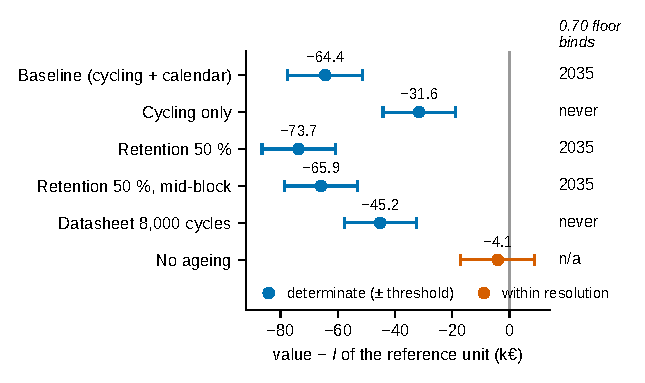
\includegraphics[width=0.90\textwidth]{fig3_ageing_arms_v2.pdf}
    \caption{Investment margins of the reference unit under alternative ageing calibrations. Bars show determinacy thresholds. Annotations identify the first representative year with a binding 0.70 state-of-health floor; ``never'' indicates an inactive floor throughout the horizon.}
    \label{fig:res_ageing}
\end{figure}
\DIFaddend 

\DIFdelbegin \DIFdel{Both coordinated configurations eliminate the voltage violation through system-wide flexibility activation. This suggests that, in }\DIFdelend \DIFaddbegin \begin{table}[htbp!]
    \centering
    \caption{Investment margins and operating indicators
    of the reference unit under alternative ageing calibrations.}
    \label{tab:res_ageing}
    \footnotesize
    \setlength{\tabcolsep}{3pt}
    \begin{tabular}{l r r c r r}
        \toprule
        Calibration
        & \shortstack{Value $- I$\\(k\euro{})}
        & \shortstack{Threshold\\(k\euro{})}
        & \shortstack{Binding\\year}
        & $AE$
        & EFC/day \\
        \midrule
        Baseline (cycling + calendar)
            & $-$64.4 & 13.1 & 2035 & 0.793 & 0.86 \\
        Cycling only
            & $-$31.6 & 12.6 & never & 0.888 & 1.19 \\
        Retention 50\,\%
            & $-$73.7 & 12.8 & 2035 & 0.786 & 0.76 \\
        Retention 50\,\%, mid-block
            & $-$65.9 & 12.9 & 2035 & 0.836 & 0.76 \\
        Datasheet 8\,000 cycles
            & $-$45.2 & 12.6 & never & 0.834 & 1.13 \\
        No ageing$^{w}$
            & $-$4.1 & 12.9 & n/a & 1.000 & 1.29 \\
        \midrule
        Baseline, 0.50 floor
            & $-$59.5 & 12.6 & never & 0.778 & 1.08 \\
        \bottomrule
    \end{tabular}
    \par\smallskip
    \begin{minipage}{\linewidth}
        \footnotesize\raggedright
        \textit{Note:} $I=318.0$~k\euro{}. $^{w}$: margin within numerical resolution; all other margins are determinate.
        Thresholds follow Subsection~\ref{subsubsec:certification}. Binding year denotes the first representative year in which the state-of-health floor binds. The floor is 0.70, except in the final row, where it is 0.50. 
        ``Never'' indicates an inactive floor throughout the horizon; n/a: not applicable.
        $AE$ is the present-value-weighted available-energy fraction; EFC/day denotes equivalent full cycles per day.
    \end{minipage}
\end{table}


    \DIFadd{The operational results also distinguish the effect of degradation from that of the imposed end-of-life floor. In the single-scenario configuration the 0.70 floor first binds in 2035 under the baseline calibration and both variants of the 50\% retention calibration, but remains inactive throughout the horizon under the cycling-only and 8}{\DIFadd{,}}\DIFadd{000-cycle datasheet calibrations; in the multi-scenario evaluation of Subsection~\ref{subsec:res_multiscenario}, with its three-year blocks, }\DIFaddend the \DIFdelbegin \DIFdel{absence of coordination, maintaining compliance with voltage limits would likely require conventional network reinforcement. Coordinated operation therefore emerges as a non-wire alternative capable of mitigating voltage problems without immediate conventional reinforcement. This is particularly relevant in systems with growing DER penetration, where improved operational coordination may defer or reduce the need for traditional grid reinforcements}\DIFdelend \DIFaddbegin \DIFadd{baseline floor binds in 2037. Lowering the baseline floor from 0.70 to 0.50 increases cycling by 0.18, 0.20 and 0.27 equivalent full cycles per day in 2025, 2030 and 2035, respectively. Nevertheless, the resulting increase in storage value is only 4.9~k}\euro{}\DIFadd{, within numerical resolution, and the unit still incurs a determinate shortfall of 59.5~k}\euro{}\DIFadd{. Thus, relaxing the end-of-life floor permits greater utilisation but does not restore the economic viability of the reference unit under the baseline assumptions. The negative investment margin persists across the tested ageing calibrations, and under the baseline calibration at both floor settings.
}



    \DIFadd{Figure~\ref{fig:res_soc_soh} shows how degradation reaches the dispatch. Panel~(a) gives the stored energy of the reference unit over the four representative days of 2025 and 2035 under the baseline calibration: the unit cycles once or twice a day across the usable band, reaching the 90\,\% limit of its available energy on every day and the 10\,\% limit on six of the eight (the Winter days stop at 14--15\,\%), and in 2035, with the state of health at the 0.70 floor, the usable band has narrowed from 0.70 to 0.56~MWh. Panel~(b) gives the end-of-block state of health under the seven calibrations: the baseline and both 50\,\% retention calibrations reach the floor in the 2035 block, the cycling-only and datasheet calibrations do not, and the 0.50 floor lets the baseline calibration continue to 0.68}\DIFaddend .


%DIF <  Operational costs
\DIFdelbegin \subsubsection{\DIFdel{Operational Costs}}
%DIFAUXCMD
\addtocounter{subsubsection}{-1}%DIFAUXCMD
\DIFdelend \DIFaddbegin \begin{figure}[htbp!]
    \centering
    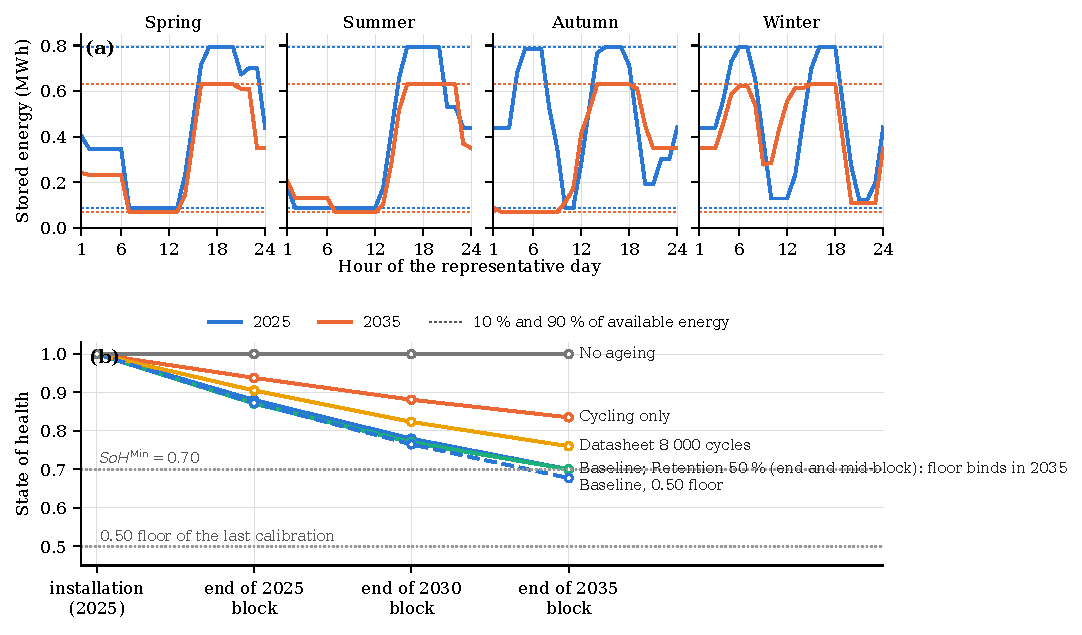
\includegraphics[width=1.00\textwidth]{fig_soc_soh_reference_unit.pdf}
    \caption{Storage operation and degradation of the reference unit (node~7, 0.25~MVA / 1~MWh, installed in 2025): (a) stored energy over the four representative days of 2025 and 2035 under the baseline calibration, with the 10\,\% and 90\,\% limits of the available energy of each year; (b) state of health at the end of each representative block under the calibrations of Table~\ref{tab:ageing_calibrations}, with the 0.70 end-of-life floor and the 0.50 floor of the last calibration. Values are read from the certified evaluation records.}
    \label{fig:res_soc_soh}
\end{figure}
\DIFaddend 

\DIFdelbegin \DIFdel{As shown in Table~[\texttt{tab:cs3\_results\_operational\_planning\_summary}], coordinated operation consistently reduces total operating costs relative to uncoordinated operation. 
    The additional benefit of shared ESS deployment becomes more pronounced in the later years of the planning horizon, when higher RES penetration amplifies flexibility needs.
    By 2037, cost reductions reach 16.58\% under coordination without shared ESSs and 18.25\% when shared ESSs are included, showing that shared storage enhances the economic value of coordinated operation.
Figure~[\texttt{fig:cs3\_results\_operational\_costs}] illustrates the evolution of operational costs by representative year, representative day, and test case, disaggregated into conventional generation }\DIFdelend %DIF >  --------------------------------------------------------------------------------------------------------------------
\DIFaddbegin \subsection{\DIFadd{Value of Coordination}}
\label{subsec:res_coordination}


    \DIFadd{Figure~\ref{fig:res_benchmark} and Table~\ref{tab:res_benchmark} compare coordinated operation with the passive and price-taker arrangements defined in Section~\ref{sec:case_settings}. Both static arrangements prohibit reverse active-power flow from each DN to the TN. 
    All three arrangements are evaluated without shared storage using the same cost function $Q$, excluding the contracted interface settlement.
    The price-taker and passive arrangements incur 13.9\% }\DIFaddend and \DIFdelbegin \DIFdel{flexibility procurement components. }\DIFdelend \DIFaddbegin \DIFadd{36.9\% higher discounted operating costs than coordinated operation, respectively.
    Coordination provides operating savings of 90.9~M}\euro{} \DIFadd{relative to the price-taker arrangement, the less costly static benchmark.
}\DIFaddend 


\DIFdelbegin %DIFDELCMD < \begin{figure}[htbp]
%DIFDELCMD <     \centering
%DIFDELCMD <     \includegraphics[width=0.95\textwidth]{results_operational_cost_multi_year.pdf}
%DIFDELCMD <     \caption{Operational costs by representative year, representative day, and test case.}
%DIFDELCMD <     \label{fig:cs3_results_operational_costs}
%DIFDELCMD < \end{figure}
%DIFDELCMD < %%%
\DIFdelend \DIFaddbegin \begin{table}[htbp!]
    \centering
    \caption{Operating costs and RES curtailment without shared storage.}
    \label{tab:res_benchmark}
    \footnotesize\setlength{\tabcolsep}{3pt}
    \begin{tabular}{l c c c c}
        \toprule
        Arrangement & $Q$ (k\euro) & $\Delta Q$ (k\euro, \%) & TN curt.\ (GWh) & DN curt.\ (GWh) \\
        \midrule
        Coordinated     & 653\,873.7 (71.9) & ---                & ---   & ---   \\
        Price-taker NRF & 744\,770.3 (0.0)  & 90\,896.6 (13.9)   & 807.6 & 0.6   \\
        Passive NRF     & 895\,049.9 (25.8) & 241\,176.2 (36.9)  & 781.7 & 201.2 \\
        \bottomrule
    \end{tabular}
    \par\smallskip
    \begin{minipage}{\linewidth}
        \footnotesize\raggedright
        \textit{Note:}
        NRF denotes prohibition of DN-to-TN active-power flow.
        Static costs are the lowest obtained from three solver starts.
        Parentheses show the coordinated evaluation's reproducibility band or the static arrangement's cost range across starts.
        $\Delta Q$ denotes cost above coordinated operation; percentages are relative to the coordinated cost.
        Curtailment is day-weighted. Dashes denote unreported quantities.
    \end{minipage}
\end{table}
\DIFaddend 

\DIFdelbegin \DIFdel{Although uncoordinated operationmay occasionally yield lower apparent operating costs in isolated representative days during the early years, these outcomes are associated with unresolved technical infeasibilities, notably voltage-limit violations (Subsection~[\texttt{subsubsec:network\_violations}]). They should therefore not be interpreted as economically preferable operating points from a system-planning perspective}\DIFdelend \DIFaddbegin \begin{figure}[htbp!]
    \centering
    \includegraphics[width=1.00\textwidth]{fig5_benchmark.pdf}
    \caption{Comparison of operating costs without shared storage:
    (a) costs under coordinated, price-taker and passive operation;
    (b) contributions of TN generation and DN flexibility costs to the cost difference between the price-taker and coordinated arrangements.
    The contracted interface settlement is excluded.}
    \label{fig:res_benchmark}
\end{figure}


    \DIFadd{Figure~\ref{fig:res_benchmark} attributes 77.2\% of the cost difference between the price-taker and coordinated arrangements to TN conventional generation and 22.8\% to DN flexibility}\DIFaddend . \DIFaddbegin \DIFadd{Under price-taker operation, DN renewable curtailment is only 0.6~GWh, while TN curtailment reaches 807.6~GWh. These results illustrate why wholesale-price signals alone may not align distribution flexibility with transmission operating conditions.
}\DIFaddend 



    %DIF <  RES generation
\DIFdelbegin \subsubsection{\DIFdel{RES Generation}}
%DIFAUXCMD
\addtocounter{subsubsection}{-1}%DIFAUXCMD
%DIFDELCMD < 

%DIFDELCMD < %%%
\DIFdel{Table~[\texttt{tab:cs3\_results\_operational\_planning\_summary}] shows that the benefits of }\DIFdelend \DIFaddbegin \DIFadd{The comparison also reflects differences in interface restrictions. Both static arrangements prohibit DN-to-TN active-power flow, whereas coordinated operation uses reverse flow in four representative interface-hours. When this restriction was removed from the static arrangements, TN dispatch runs could not accommodate the prescribed DN exchanges in one of twelve representative year--season blocks for passive operation and eight for price-taker operation (Table~S5 of the supplementary material). To separate the two effects, }\DIFaddend coordinated operation \DIFdelbegin \DIFdel{for renewable integration become substantial from 2031 onward, when rising RES penetration leads to significant curtailment under uncoordinated operation }\DIFdelend \DIFaddbegin \DIFadd{was re-evaluated with the same no-reverse-flow restriction imposed on the consensus exchange. The restriction raises the coordinated cost by 20.5~k}\euro{}\DIFadd{, a determinate increase at 1.62 times its threshold, which is 0.02\,\% of the 90.9~M}\euro{} \DIFadd{saving: the saving relative to the price-taker arrangement is 12.2\,\% with reverse flow enabled and 12.2\,\% with it prohibited. The coordination benefit reported here does not depend on the interface restriction; it applies to the specific benchmark arrangements defined in Section~\ref{sec:case_settings}}\DIFaddend .
\DIFdelbegin \DIFdel{In 2037, curtailment is reduced by 88.54\% under coordination without shared ESSs and by 92.16\% when shared ESSs are included. Figures~[\texttt{fig:cs3\_results\_res\_generation}] and~[\texttt{fig:cs3\_results\_res\_curtailment}] provide a more detailed view of RES generation and curtailment; as noted above, curtailment is reported in MVAh because it is measured with respect to apparent power.
}\DIFdelend 


\DIFdelbegin %DIFDELCMD < \begin{figure*}[htbp!]
%DIFDELCMD <     \centering
%DIFDELCMD <     \begin{subfigure}[b]{0.90\textwidth}  
%DIFDELCMD <         \centering 
%DIFDELCMD <         \includegraphics[width=\textwidth]{results_res_generation_active_power_multi_year.pdf}
%DIFDELCMD <         \caption{Active energy.}
%DIFDELCMD <     \end{subfigure}
%DIFDELCMD <     \hfill
%DIFDELCMD <     \begin{subfigure}[b]{0.90\textwidth}   
%DIFDELCMD <         \centering 
%DIFDELCMD <         \includegraphics[width=\textwidth]{results_res_generation_reactive_power_multi_year.pdf}
%DIFDELCMD <         \caption{Reactive energy.}
%DIFDELCMD <         \label{fig:cs3_results_res_generation_reactive}
%DIFDELCMD <     \end{subfigure}
%DIFDELCMD <     \caption{RES generation by representative year, representative day, and test case.}
%DIFDELCMD <     \label{fig:cs3_results_res_generation}
%DIFDELCMD < \end{figure*}
%DIFDELCMD < %%%
\DIFdelend %DIF >  --------------------------------------------------------------------------------------------------------------------
\DIFaddbegin \subsection{\DIFadd{Multi-Scenario Evaluation}}
\label{subsec:res_multiscenario}
\DIFaddend 


    \DIFdelbegin %DIFDELCMD < \begin{figure}[htbp]
%DIFDELCMD <     \centering
%DIFDELCMD <     \includegraphics[width=0.90\textwidth]{results_res_generation_curtailment_multi_year.pdf}
%DIFDELCMD <     \caption{RES curtailment by representative year, representative day, and test case.}
%DIFDELCMD <     \label{fig:cs3_results_res_curtailment}
%DIFDELCMD < \end{figure}
%DIFDELCMD < 

%DIFDELCMD < %%%
\DIFdel{Figure~[\texttt{fig:cs3\_results\_res\_generation\_reactive}] further highlights the benefits of coordinated operation. Under uncoordinated operation, RES generators absorb large amounts of reactive power in an attempt to support transmission-level voltage regulation, yet these efforts remain insufficient to prevent voltage violations (Figure~[\texttt{fig:cs3\_results\_bus\_voltage\_violation}]). By contrast, coordinated operation enables a more efficient allocation of reactive power support, allowing RES generators to operate closer to unitary power factor. This indicates that coordinated flexibility activation becomes increasingly important for sustaining high RES integration as system stress rises over the planning horizon. This effect also helps explain why the value of shared ESS deployment increases toward the end of }\DIFdelend \DIFaddbegin \DIFadd{The reference unit and the plan without storage were evaluated for all nine combinations of three market scenarios and three load and renewable-generation scenarios, using five representative three-year blocks. The planning search was not repeated. In this configuration the operating cost $Q$ includes the deviation component of }\DIFaddend the \DIFdelbegin \DIFdel{planning horizon: as RES penetration rises, the coupled system requires greater flexibility not only in active power but also in reactive power support and voltage management. Shared ESSs provide an additional controllable resource that can relieve these growing network stresses.
}\DIFdelend \DIFaddbegin \DIFadd{interface settlement and the commitment premium of Subsection~\ref{subsubsec:commitment} (together about 3\,\% of $Q$ at the plan without storage); the contracted settlement is excluded, as in the single-scenario configuration. As shown in Table~\ref{tab:res_multiscenario}, the reference unit provides estimated discounted operating savings of 236.7~k}\euro{} \DIFadd{against an investment cost of 318.0~k}\euro{}\DIFadd{. The resulting shortfall of 81.3~k}\euro{} \DIFadd{exceeds the reported numerical resolution of 18.0~k}\euro{}\DIFadd{. These evaluations used the residual-based stopping criterion described in \ref{app:admm_updated_stopping} and were not certified under the rule of Subsection~\ref{subsubsec:certification}.
}\DIFaddend 



    %DIF <  Flexibility procurement
\DIFdelbegin %DIFDELCMD < 

%DIFDELCMD < %%%
%DIF < \subsubsection{Flexibility Procurement}
%DIFDELCMD < 

%DIFDELCMD < %%%
%DIF < Figure~[\texttt{fig:cs3\_results\_flexibility\_usage}] reports the total flexibility services procurement across representative years, days, and test cases.
%DIF < As RES penetration increases over the planning horizon, demand-side flexibility becomes progressively more important, particularly in spring and summer. These results confirm that coordinated operation enables a more effective utilization of existing flexibility resources, aligning flexibility activation with evolving generation patterns and reinforcing the role of ADNs as key contributors to system-wide balancing and voltage support.
%DIFDELCMD < 

%DIFDELCMD < %%%
%DIF < \begin{figure*}[htbp!]
%DIF <     \centering
%DIF <     \begin{subfigure}[b]{0.90\textwidth}  
%DIF <         \centering 
%DIF <         \includegraphics[width=\textwidth]{results_flexibility_active_power_multi_year.pdf}
%DIF <         \caption{Active energy.}
%DIF <     \end{subfigure}
%DIF <     \hfill
%DIF <     \begin{subfigure}[b]{0.90\textwidth}   
%DIF <         \centering 
%DIF <         \includegraphics[width=\textwidth]{results_flexibility_reactive_power_multi_year.pdf}
%DIF <         \caption{Reactive energy.}
%DIF <     \end{subfigure}
%DIF <     \caption{Flexibility procurement per representative year and day.} 
%DIF <     \label{fig:cs3_results_flexibility_usage}
%DIF < \end{figure*}
%DIFDELCMD < 

%DIFDELCMD < %%%
\subsection{\DIFdel{Impact of Planning Horizon Discretization}}
%DIFAUXCMD
\addtocounter{subsection}{-1}%DIFAUXCMD
%DIFDELCMD < 

%DIFDELCMD < %%%
\DIFdel{Temporal discretization strongly influences degradation modeling accuracy and, consequently, ESS investment decisions. This issue is particularly relevant in storage planning because battery capacity can degrade substantially over relatively short operating horizons}\DIFdelend \DIFaddbegin \DIFadd{A fit to the continued objective trajectory of the plan without storage estimated a further cost decrease of 6.2~k}\euro{}\DIFadd{. Accounting for this decrease alone would reduce the estimated storage value from 236.7 to 230.5~k}\euro{}\DIFadd{, corresponding to values approximately 7--9\,\% below the single-scenario value. This range reflects estimated remaining movement in the no-storage evaluation and is not a certified interval. The configurations also differ in temporal discretisation and commitment-cost treatment, so the lower value cannot be attributed solely to scenario uncertainty}\DIFaddend .


\DIFdelbegin \DIFdel{To assess this effect, two alternative planning configurations are evaluated in addition to the baseline case with a 3-year discretization step:
}%DIFDELCMD < \begin{itemize}
\begin{itemize}%DIFAUXCMD
%DIFDELCMD <     \item %%%
\item%DIFAUXCMD
\DIFdel{a 5-year discretization, which reduces temporal resolution while keeping the remaining modeling assumptions unchanged;
    }%DIFDELCMD < \item %%%
\item%DIFAUXCMD
\DIFdel{a 1-year discretization, which increases temporal resolution to annual intervals. Due to memory limitations, the number of market-price and operational scenarios is reduced to three in each case, while maintaining four representative days per year and three investment scenarios.
}
\end{itemize}%DIFAUXCMD
%DIFDELCMD < \end{itemize}
%DIFDELCMD < %%%
\DIFdelend \DIFaddbegin \begin{table}[htbp!]
    \centering
    \caption{Multi-scenario evaluation of the reference unit (node~7, 0.25~MVA / 1~MWh, installed in 2025).}
    \label{tab:res_multiscenario}
    \footnotesize\setlength{\tabcolsep}{5pt}
    \begin{tabular}{l c}
        \toprule
        Quantity & Value \\
        \midrule
        Discounted operating savings & 236.7~k\euro{} \\
        Investment cost & 318.0~k\euro{} \\
        Investment margin & $-$81.3~k\euro{} \\
        Reported numerical resolution & 18.0~k\euro{} \\
        Single-scenario operating savings & 253.5~k\euro{} \\
        Value ratio at stopping & 0.934 \\
        Value ratio after estimated continuation adjustment & 0.909 \\
        \bottomrule
    \end{tabular}
    \par\smallskip
    \begin{minipage}{\linewidth}
        \footnotesize\raggedright
        \textit{Note:}
        Operating savings and investment margin are reported at the residual-based stopping point; the multi-scenario evaluations are uncertified.
        Operating costs follow \eqref{eq:recourse_value}.
        Ratios use the single-scenario operating savings as the denominator.
        The adjusted ratio accounts only for the estimated further decrease of 6.2~k\euro{} in the no-storage cost, obtained from a damped-cosine fit; the reference unit's evaluated cost is held fixed.
    \end{minipage}
\end{table}
\DIFaddend 

\DIFdelbegin \DIFdel{Consequently, the 1-year discretization case should be interpreted primarily as a sensitivity test on temporal resolution rather than as a perfectly like-for-like comparison with the baseline configuration.
}\DIFdelend %DIF >  --------------------------------------------------------------------------------------------------------------------
\DIFaddbegin \subsection{\DIFadd{Investment Year and Discount Rate}}
\label{subsec:res_sensitivities}
\DIFaddend 


    \DIFdelbegin \DIFdel{Table~[\texttt{tab:cs3\_shared\_ess\_investment\_plan\_5year\_discretization}] reports the expected shared ESS investment plan obtained under the coarser 5-year discretization. In this case, rather than allocating the entire budget to a single shared ESS at node~7, as in the baseline case, the investment is split between two units installed in 2025: a larger system }\DIFdelend \DIFaddbegin \DIFadd{Deferring installation does not make the reference investment economically viable (Table~\ref{tab:res_year_ladder}(a)). Later installations have fewer operating years within the horizon and receive larger terminal salvage credits. After accounting for this credit, total discounted costs remain 54.5--64.4~k}\euro{} \DIFadd{above those of the plan without storage across the three installation years. The credit reduces the cost difference between installation in 2030 and 2035 to within numerical resolution, so neither year can be identified as preferable on this basis. The larger units evaluated }\DIFaddend at node~7, \DIFdelbegin \DIFdel{rated at 1.54}\DIFdelend \DIFaddbegin \DIFadd{comprising 0.5}\DIFaddend ~MVA / \DIFdelbegin \DIFdel{3.09~MWh , and a smaller one at node~9, rated at 0.10~MVA / 0.20~MWh. This result illustrates that coarser temporal aggregation can affect both the spatial allocation and sizing of shared ESSs}\DIFdelend \DIFaddbegin \DIFadd{1~MWh and 0.5~MVA / 2~MWh, also remain more expensive than the plan without storage when installed in either year, before and after salvage (Table~\ref{tab:appE_claims}, rows~17--20)}\DIFaddend .


\DIFdelbegin %DIFDELCMD < \begin{table}[htbp!]
%DIFDELCMD <     \centering
%DIFDELCMD <     \caption{Shared ESS investment plan for the 5-year discretization case.}
%DIFDELCMD <     \centering
%DIFDELCMD <     \begin{tabular}{cl ccc}
%DIFDELCMD <         \toprule
%DIFDELCMD <         Node & Parameter                   & 2025 & 2030 & 2035\\ 
%DIFDELCMD <         \midrule
%DIFDELCMD <         7 & $S^{\text{Inv}}_{e,y}$, [MVA]  & 1.54  & - & - \\
%DIFDELCMD <         ~ & $E^{\text{Inv}}_{e,y}$, [MWh]  & 3.09  & - & - \\
%DIFDELCMD <         \midrule
%DIFDELCMD <         9 & $S^{\text{Inv}}_{e,y}$, [MVA]  & 0.10  & - & - \\
%DIFDELCMD <         ~ & $E^{\text{Inv}}_{e,y}$, [MWh]  & 0.20  & - & - \\
%DIFDELCMD <         \midrule
%DIFDELCMD <         - & Inv., [NPV M\euro]             & 1.00  & 0.00  & 0.00 \\
%DIFDELCMD <         \bottomrule
%DIFDELCMD <     \end{tabular}
%DIFDELCMD <     \label{tab:cs3_shared_ess_investment_plan_5year_discretization}
%DIFDELCMD < \end{table}
%DIFDELCMD < %%%
\DIFdelend \DIFaddbegin \begin{table}[htbp!]
    \centering
    \caption{Installation-year and discount-rate sensitivities of the reference unit (node~7, 0.25~MVA / 1~MWh).}
    \label{tab:res_year_ladder}
    \footnotesize\setlength{\tabcolsep}{5pt}
    \begin{tabular}{l c c c}
        \multicolumn{4}{l}{(a) Installation year, 2\,\% discount rate} \\
        \toprule
        Investment year & $M$ gross (k\euro) & Salvage (k\euro) & $M$ net (k\euro) \\
        \midrule
        2025 (reference) & 64.4  & 0.0  & 64.4 \\
        2030             & 68.5  & 11.8 & 56.7 \\
        2035             & 111.0 & 56.5 & 54.5 \\
        2035 $-$ 2030    & 42.5  & ---  & $-$2.3 \\
        \bottomrule
        \multicolumn{4}{c}{} \\
        \multicolumn{4}{l}{(b) Discount rate, installation in 2025} \\
        \toprule
        Rate (\%) & Value (k\euro) & Value $- I$ (k\euro) & Threshold (k\euro) \\
        \midrule
        0 & 277.1 & $-$40.8  & 15.9 \\
        2 & 253.5 & $-$64.4  & 13.1 \\
        5 & 225.2 & $-$92.7  & 13.1 \\
        8 & 203.4 & $-$114.6 & 13.1 \\
        \bottomrule
    \end{tabular}
    \par\smallskip
    \begin{minipage}{\linewidth}
        \footnotesize\raggedright
        \textit{Note:}
        (a) $M = I + Q(\boldsymbol{x}) - Q(\boldsymbol{0})$ is the cost increase relative to the plan without storage; net cost deducts the terminal salvage credit \eqref{eq:salvage_credit}; the final row compares installation in 2035 with 2030: the gross difference is determinate, the net difference within numerical resolution (threshold: 12.3~k\euro{}).
        (b) Investment cost $I=318.0$~k\euro{}, paid in 2025; all investment margins are determinate under the criteria of Subsection~\ref{subsubsec:certification}; rates other than 2\,\% reweight the annual operating costs of the 2\,\% evaluations without re-optimising dispatch.
    \end{minipage}
\end{table}
\DIFaddend 


    \DIFdelbegin \DIFdel{Table~[\texttt{tab:cs3\_shared\_ess\_specs\_5year\_discretization}] reports the expected evolution of energy capacity and SoH of the two installed ESSs. The ESS installed at node~7 reaches an end-of-life SoH of 50.80\%, closely matching the 49.62\% obtained with the 3-year discretization step. By contrast, the ESS installed at node~9 exhibits substantially higher degradation, reflecting more intensive cycling. This result highlights the sensitivity of ESS planning to discretization choices and underscores the importance of accurately capturing degradation effects. }\DIFdelend \DIFaddbegin \DIFadd{The reference unit has a negative investment margin at all four evaluated discount rates (Table~\ref{tab:res_year_ladder}(b)). Its shortfall increases from 40.8~k}\euro{} \DIFadd{without discounting to 114.6~k}\euro{} \DIFadd{at 8\,\%, since investment is paid in 2025 while operating savings accrue over the horizon. Rates other than 2\,\% were evaluated by reweighting the annual costs of the 2\,\% evaluations without re-optimising operation. This reweighting is exact for the plan without storage but approximate for the reference unit, whose operation is coupled across years through battery degradation.
}\DIFaddend 



\DIFdelbegin %DIFDELCMD < \begin{table}[htbp!]
%DIFDELCMD <     \centering
%DIFDELCMD <     \caption{Available capacity and SoH of the shared ESSs in the 5-year discretization case.}
%DIFDELCMD <     \begin{tabular}{cl ccc}
%DIFDELCMD <         \toprule
%DIFDELCMD <         Node ID & Parameter & 2025 & 2030 & 2035\\ 
%DIFDELCMD <         \midrule
%DIFDELCMD <         7 & $E^{\text{Av}}_{e,y}$, [MWh]    & 2.27	    & 1.83	    & 1.57\\
%DIFDELCMD <         ~ & SoH, [\%]                       & 73.48\%   & 59.15\%   & 50.80\%\\
%DIFDELCMD <         \midrule
%DIFDELCMD <         9 & $E^{\text{Av}}_{e,y}$, [MWh]    & 0.13      & 0.10      & 0.07\\ 
%DIFDELCMD <         ~ & SoH, [\%]                       & 60.76\%   & 50.91\%   & 38.43\%\\ 
%DIFDELCMD <         \bottomrule
%DIFDELCMD <     \end{tabular}
%DIFDELCMD <     \label{tab:cs3_shared_ess_specs_5year_discretization}
%DIFDELCMD < \end{table}
%DIFDELCMD < %%%
\DIFdelend %DIF >  --------------------------------------------------------------------------------------------------------------------
\DIFaddbegin \subsection{\DIFadd{Numerical Performance, Scope and Limitations}}
\label{subsec:res_certification}
\DIFaddend 


    \DIFdelbegin \DIFdel{Tables~[\texttt{tab:cs3\_shared\_ess\_investment\_plan\_1year\_discretization}] and ~[\texttt{tab:cs3\_shared\_ess\_specs\_1year\_discretization}] report the investment plan and }\DIFdelend \DIFaddbegin \DIFadd{In the main single-scenario evaluation campaign, 32 of 42 recourse evaluations satisfied the numerical acceptance criteria of Subsection~\ref{subsubsec:certification}; the remaining ten are reported as uncertified. On the reference evaluations, the objective changed by a further 15--21~k}\euro{} \DIFadd{after the residual-based stopping criterion had been met, motivating the additional checks on objective stability and interface consistency. In three evaluations continued beyond certification, further objective changes were at most $0.9\tau$. Detailed statistics, individual evaluation statuses and reproducibility records are provided in \ref{app:results}.
}



    \DIFadd{The sensitivity of the decisive comparisons to the coordination penalties was tested by re-evaluating the plan without storage and }\DIFaddend the \DIFdelbegin \DIFdel{evolution of available capacity and SoH, respectively, for the 1-year discretization case.
In this case, the investment plan is identical to that obtained in the baseline case: a single shared ESS rated at 1.62~MVA/3.24~MWh is installed at node~7 in 2025.
}\DIFdelend \DIFaddbegin \DIFadd{reference unit, at the base and at twice the base flexibility price, with every initial penalty parameter halved and doubled. All eight re-evaluations certified. Across the three penalty settings, the operating-cost difference between the two plans varied by 1.6~k}\euro{} \DIFadd{at the base price and 1.5~k}\euro{} \DIFadd{at twice the base price, about 0.12 of its determinacy threshold in each case, and every sign and verdict was unchanged; seven of the eight re-evaluations fell inside the acceptance window of the corresponding frozen evaluation and the eighth lay 0.7~k}\euro{} \DIFadd{above it. The check covers the penalty schedule, not the start of the coordination: a different initialisation could in principle reach a different local solution, and the limitation below stands.
}\DIFaddend 



    \DIFdelbegin %DIFDELCMD < \begin{table}[htbp!]
%DIFDELCMD <     \centering
%DIFDELCMD <     \caption{Shared ESS investment plan for the 1-year discretization case.}
%DIFDELCMD <     \begin{tabular}{cl ccc c c}
%DIFDELCMD <         \toprule
%DIFDELCMD <         Node & Parameter                   & 2025 & 2026 & 2027 & \ldots & 2039\\ 
%DIFDELCMD <         \midrule
%DIFDELCMD <         7 & $S^{\text{Inv}}_{e,y}$, [MVA]  & 1.62  & - & - & \ldots & - \\
%DIFDELCMD <         ~ & $E^{\text{Inv}}_{e,y}$, [MWh]  & 3.24  & - & - & \ldots & - \\
%DIFDELCMD <         \midrule
%DIFDELCMD <         - & Inv., [NPV M\euro]             & 1.00  & 0.00  & 0.00 & \ldots & 0.00 \\
%DIFDELCMD <         \bottomrule
%DIFDELCMD <     \end{tabular}
%DIFDELCMD <     \label{tab:cs3_shared_ess_investment_plan_1year_discretization}
%DIFDELCMD < \end{table}
%DIFDELCMD < %%%
\DIFdelend \DIFaddbegin \DIFadd{Figure~\ref{fig:res_q_cycle} illustrates two numerical outcomes. For the plan without storage }[\DIFadd{panel (a)}]\DIFadd{, the objective at the residual-based stopping point (cycle 132) differs by 15.0~k}\euro{} \DIFadd{from its value at certification (cycle 181). For the reference unit at 1.5 times the base flexibility price }[\DIFadd{panels (b) and (c)}]\DIFadd{, the objective stabilises but the priced interface-consensus gap remains outside the acceptance band, so the evaluation is reported as uncertified.
}\DIFaddend 


\DIFdelbegin %DIFDELCMD < \begin{table}[htbp!]
%DIFDELCMD <     \centering
%DIFDELCMD <     \caption{Available capacity and SoH of the shared ESS in the 1-year discretization case.}
%DIFDELCMD <     \resizebox{1.00\textwidth}{!}{
%DIFDELCMD <         \begin{tabular}{l ccc c ccc}
%DIFDELCMD <             \toprule
%DIFDELCMD <             Parameter & 2025 & 2026 & 2027 & \ldots & 2037 & 2038 &2039\\ 
%DIFDELCMD <             \midrule
%DIFDELCMD <             $E^{\text{Av}}_{e,y}$, [MWh]    & 3.16	    & 3.07	    & 2.96   & \dots & 2.13     & 2.06    & 1.99 \\
%DIFDELCMD <             SoH, [\%]                       & 97.56\%	& 94.56\%	& 91.42\%& \dots & 65.83\%  & 63.65\% & 61.49\%\\
%DIFDELCMD <             \bottomrule
%DIFDELCMD <         \end{tabular}
%DIFDELCMD <     }
%DIFDELCMD <     \label{tab:cs3_shared_ess_specs_1year_discretization}
%DIFDELCMD < \end{table}
%DIFDELCMD < %%%
\DIFdelend \DIFaddbegin \begin{figure}[htbp!]
    \centering
    \includegraphics[width=1.00\textwidth]{fig4_q_versus_cycle.pdf}
    \caption{Numerical acceptance of two single-scenario evaluations:
    (a) objective for the plan without storage;
    (b) objective and (c) priced interface-consensus gap for the reference unit at 1.5 times the base flexibility price.
    Objectives are relative to their values at certification in (a) and at the cycle cap in (b).
    Markers $k_0$, $N$ and $k^{*}$ denote the first residual pass, residual-based stopping point and certification, respectively.
    Shading indicates the acceptance window in (a), the last 60 cycles in (b), and the gap acceptance band $\pm\tau/2$ in (c).
    Circles mark objective turning points; orange ticks indicate cycles satisfying all acceptance criteria except the interface-gap criterion.}
    \label{fig:res_q_cycle}
\end{figure}
\DIFaddend 


    \DIFdelbegin \DIFdel{These findings show that temporal discretization can materially influence investment decisions. While coarse discretization reduces computational burden, it may distort degradation dynamics and bias investment outcomes. Conversely, finer discretization improves physical fidelity at the cost of greater computational complexity}\DIFdelend \DIFaddbegin \DIFadd{The three planning searches performed 41 new recourse evaluations using the residual-based stopping rule. Plans used in the reported single-scenario comparisons were assessed separately under the numerical acceptance criteria of Subsection~\ref{subsubsec:certification}. The 42-evaluation acceptance campaign required 61.4~h of wall time over 8}{\DIFadd{,}}\DIFadd{570 ADMM cycles, with a median of 25.6~s per cycle. Evaluations were run sequentially using a single thread on an Apple M2~Max. Detailed search records and the computing environment are provided in \ref{app:results_statistics}.
}




    \textbf{\DIFadd{Interface-consensus gaps.}} \DIFadd{Some evaluations remained uncertified because the priced interface-consensus gap exceeded the acceptance tolerance despite a stable objective. This behaviour was associated with TN conventional generation at its lower bound and inactive DN flexibility, suggesting that non-unique interface marginal values may impede consensus. The affected evaluations and their diagnostic measures are listed in Table~S6; their cost comparisons are assessed using the uncertified comparison criteria of Subsection~\ref{subsubsec:certification}. Possible remedies, including an economic tie-breaker in the storage-agent objective, require further evaluation}\DIFaddend .



    \DIFdelbegin \subsection{\DIFdel{Key Insights}}
%DIFAUXCMD
\addtocounter{subsection}{-1}%DIFAUXCMD
%DIFDELCMD < 

%DIFDELCMD < %%%
\DIFdel{Overall, the results show that the value of shared ESS deployment increases as RES penetration rises and coordinated transmission--distribution operation becomes more important}\DIFdelend \DIFaddbegin \textbf{\DIFadd{Solver recoveries and numerical slacks.}} \DIFadd{Some TN solves required recovery after reaching the iteration limit. Cycles failing the prescribed local-solve quality checks are excluded from certification evidence (Table~S4). Renewable-output bounds include a numerical slack of $10^{-5}$~p.u., resulting in approximately 62~MWh-equivalent of generation above availability over the planning horizon. This excess is reported separately from RES curtailment}\DIFaddend .



    \DIFdelbegin \DIFdel{The case study yields four main insights:
}%DIFDELCMD < \begin{enumerate}[(i)]
%DIFDELCMD <     \item %%%
\DIFdel{early shared ESS deployment can be economically attractive under favorable or moderate investment-cost trajectories;
    }%DIFDELCMD < \item %%%
\DIFdel{coordinated TSO--DSO operation substantially reduces operating costs and RES curtailment, and these benefits are further enhanced by shared ESS deployment in high-stress operating conditions;
    }%DIFDELCMD < \item %%%
\DIFdel{explicitly accounting for degradation prevents overvaluation of shared ESS capacity and leads to more technically credible long-term investment decisions; and }%DIFDELCMD < \item %%%
\DIFdel{the temporal discretization adopted for the planning horizon materially affects degradation trajectories and can alter both the sizing and spatial allocation of shared ESS investments.
}%DIFDELCMD < \end{enumerate}
%DIFDELCMD < %%%
\DIFdelend \DIFaddbegin \textbf{\DIFadd{Objective drift.}} \DIFadd{The numerical acceptance criteria examine objective stability over finite windows. A slowly drifting evaluation can satisfy the monotone branch's linear extrapolation check while retaining objective changes beyond $\tau$. Certification therefore does not provide a guaranteed bound on the remaining objective movement (\ref{app:admm_updated_certification}).
}\DIFaddend 



    \DIFdelbegin \DIFdel{Taken together, these findings confirm that shared ESS planning cannot be reliably addressedthrough purely static, degradation-neutral, or single-level formulations when storage is expected to provide services across both TN and DNs}\DIFdelend \DIFaddbegin \textbf{\DIFadd{Scope of the study.}} \DIFadd{The planning search considered one installation per selected node, with a common installation year. Node-specific timing and staged expansion were not explored, although the formulation allows both. The baseline conclusion applies to the evaluated plans and does not establish global optimality. The degradation sensitivities and multi-scenario analysis evaluated fixed investment plans without repeating the planning search.
}



    \DIFadd{The operational recourse is nonconvex, and its evaluated costs may depend on initialisation and coordination settings. Numerical evidence is limited to one 108-bus test system under the single-scenario and $3 \times 3$ multi-scenario configurations, with the adopted temporal aggregation and degradation calibrations. Terminal salvage credits are excluded from the planning objective and reported only in net values. The allocation of shared-ESS degradation among operators was not addressed}\DIFaddend .


% ====================================================================================================================
%                                                      CONCLUSIONS                                                    
% ====================================================================================================================
\section{Conclusions}
\label{sec:conclusions}


    This paper presented a degradation-aware framework for planning shared \DIFdelbegin \DIFdel{ESS deployment }\DIFdelend \DIFaddbegin \DIFadd{ESSs }\DIFaddend at TN--DN interface nodes\DIFdelbegin \DIFdel{in power systems with high DER penetration. The proposed methodology integrates long-term investment planning with short-term }\DIFdelend \DIFaddbegin \DIFadd{. The two-stage stochastic formulation links investment decisions with }\DIFaddend coordinated TSO--DSO operation \DIFdelbegin \DIFdel{through a bi-level optimization architecture, allowing siting, sizing, and timing decisions to be evaluated under realistic operating conditions and investment uncertainty. 
The upper level is solved by Benders' decomposition, while the operational layer relies on the }\DIFdelend \DIFaddbegin \DIFadd{under uncertainty, while battery degradation couples storage utilisation with available capacity over the planning horizon. A derivative-free search explores discrete investment plans, which are evaluated using }\DIFaddend ADMM-based \DIFdelbegin \DIFdel{TSO--DSO coordination framework of ~\mbox{%DIFAUXCMD
\cite{simoes_2023}}\hskip0pt%DIFAUXCMD
, extended here to explicitly represent battery degradation}\DIFdelend \DIFaddbegin \DIFadd{coordination with a dedicated shared-ESS agent. Numerical acceptance criteria assess the stability of the resulting operating-cost comparisons}\DIFaddend .



    \DIFdelbegin \DIFdel{The results show that shared ESSs can provide substantial system-wide benefits when planned and operated within a coordinated TSO--DSO framework. In the }\DIFdelend \DIFaddbegin \DIFadd{In the 108-bus }\DIFaddend case study, coordinated operation \DIFdelbegin \DIFdel{with shared ESSs reduces }\DIFdelend \DIFaddbegin \DIFadd{without shared storage reduced discounted }\DIFaddend operating costs by \DIFdelbegin \DIFdel{up to 18.25\%and RES curtailment by up to 92.16\% relative to uncoordinated operation in the later years of the study horizon, while eliminating the voltage violations observed in the uncoordinated case}\DIFdelend \DIFaddbegin \DIFadd{90.9~M}\euro{} \DIFadd{(12.2\,\%) relative to the price-taker benchmark, which prohibited DN-to-TN reverse active-power flow. Under the baseline assumptions, none of the evaluated storage plans recovered its investment cost. The reference unit, comprising 0.25~MVA and 1~MWh, incurred an investment shortfall of 64.4~k}\euro{} \DIFadd{against an investment cost of 318.0~k}\euro{}\DIFaddend .
\DIFaddbegin 



    \DIFadd{Fixed-plan sensitivities showed that the reference unit's investment margin was within the numerical resolution of zero without ageing, so its sign is not resolved, and negative under all tested calibrations that included ageing. }\DIFaddend These findings \DIFdelbegin \DIFdel{indicate that shared ESSs can act as an effective non-wire alternative to conventional network reinforcement when their valueis assessed jointly across transmission and distribution levels. }%DIFDELCMD < 

%DIFDELCMD < %%%
\DIFdel{The analysis also highlights the importance of explicitly accounting for degradation in }\DIFdelend \DIFaddbegin \DIFadd{support explicitly representing degradation when estimating }\DIFaddend long-term \DIFdelbegin \DIFdel{ESS planning. In the case study, the selected ESS is intensively utilized and approaches typical end-of-life SoH thresholds by the end of the study horizon, showing that storage value and storage aging must be assessed jointly. In addition, the sensitivity analysis shows that planning-horizon discretization can materially affect ESS sizing and spatial allocation, reinforcing the need for adequate temporal resolution in degradation-sensitive planning studies. }\DIFdelend \DIFaddbegin \DIFadd{storage value. The estimated marginal break-even energy costs for 4~h storage at node~7 were below the baseline energy-capacity cost. Higher flexibility procurement prices improved the reference unit's economics, yielding positive investment margins at 1.75 and 2 times the base price. Its estimated investment margin remained negative in the multi-scenario evaluation.
}\DIFaddend 



    \DIFdelbegin \DIFdel{Future work will focus on extending the framework to additional shared flexibility resources, incorporating richer representations of }\DIFdelend \DIFaddbegin \DIFadd{Future work will extend the planning search to node-specific installation timing and staged expansion with the terminal value of the asset inside the planning objective, will seek valid lower bounds on the operational recourse through a convex relaxation of the coordinated AC model so that the distance between an evaluated plan and a bound can be reported, and will assess the scalability and numerical robustness of the coordination procedure on larger test systems. Further developments will consider richer }\DIFaddend degradation and uncertainty \DIFdelbegin \DIFdel{, and developing tighter approximation and decomposition strategies to improve numerical robustness}\DIFdelend \DIFaddbegin \DIFadd{models, other shared flexibility resources, and the allocation of battery degradation among operators}\DIFaddend .


\DIFdelbegin %DIFDELCMD < \appendix
%DIFDELCMD < 

%DIFDELCMD < %%%
\DIFdelend % ====================================================================================================================
%                                                        APPENDIX                                                     
% ====================================================================================================================

\DIFaddbegin \appendix

\DIFaddend \section{TSO--DSO Coordinated Operational Planning}
\label{app:admm_updated}


    This appendix \DIFdelbegin \DIFdel{describes the extensions introduced to the consensus-based ADMM framework proposed in~\mbox{%DIFAUXCMD
\cite{simoes_2023} }\hskip0pt%DIFAUXCMD
to incorporate the shared ESS degradation subproblem. While the original formulation coordinated TSO and DSO operational planning through consensus on interface variables, the present work introduces an additional shared ESS agentresponsible for modeling capacity degradation.
For completeness andreproducibility, the updated algorithm and subproblem formulation are provided below.
    }\DIFdelend \DIFaddbegin \DIFadd{states the coordination procedure that evaluates a candidate plan, as implemented: the consensus ADMM of~\mbox{%DIFAUXCMD
\cite{simoes_2023} }\hskip0pt%DIFAUXCMD
extended with the shared-ESS agent of Subsection~\ref{subsec:subproblem}. It is a three-agent, global-variable consensus on the storage schedule, combined with a pairwise consensus on each TN--DN interface, run as a sweep (DSOs, then TSO, then the storage agent) that is Gauss--Seidel on the interface channels and, on the storage channel, a global-variable consensus in which all three agents solve against the same $z$ before it is updated; the penalty parameters follow residual balancing, and the iteration uses Anderson acceleration and a tightened interior-point tail.
    The stopping test is stated here; the certification rule that decides when an evaluation's value may be used is Subsection~\ref{subsubsec:certification}.
}\DIFaddend 


\subsection{\DIFdelbegin \DIFdel{Updated Algorithm}\DIFdelend \DIFaddbegin \DIFadd{Agents, Blocks and Consensus Variables}\DIFaddend }
\DIFdelbegin %DIFDELCMD < \label{app:admm_updated_algorithm}
%DIFDELCMD < %%%
\DIFdelend \DIFaddbegin \label{app:admm_updated_agents}
\DIFaddend 


    \DIFdelbegin \DIFdel{Algorithm~\ref{alg:operational_planning_degradation} presents the updated pseudo-code of }\DIFdelend \DIFaddbegin \DIFadd{A }\emph{\DIFadd{block}} \DIFadd{is one representative year $y$ and one representative day $d$. The TSO holds one network model per block; each DSO $i \in N^I$ holds one model of its DN per block; every scenario of the block lives inside the same model, with the objective weighted by the scenario probabilities. The shared-ESS agent holds one model per interface node $e \in E^S$ spanning all years, days and hours, and no scenario index. Each network block objective is divided by a common scale $\sigma$ and multiplied by its block weight $w_{y,d} = Y_y D_d (1+r)^{-(y-y_0)}$, so that every block is solved in the same units and the sum over blocks, after the exclusions of Subsection~\ref{subsubsec:certification}, is the discounted operating cost of \eqref{eq:recourse_value}.
}



    \DIFadd{Three families of consensus variables couple the agents. On the interface of DN $i$: the voltage $V^{\text{I}}_{i,y,d,t}$ and the active and reactive power exchanges $P^{\text{I}}_{i,y,d,t}$, $Q^{\text{I}}_{i,y,d,t}$, shared by the TSO and DSO~$i$ ($P^{\text{I}}$ is positive from the TN to DN~$i$ and is the DN's import at the interface net of the co-located shared ESS, whose schedule has its own channel); in }\DIFaddend the \DIFdelbegin \DIFdel{consensus ADMM-based TSO--DSO coordinated operational planning framework introduced in ~\mbox{%DIFAUXCMD
\cite{simoes_2023}}\hskip0pt%DIFAUXCMD
, extended here to include the shared ESS operation subproblem described in Subsection~\ref{subsec:subproblem}. The extended coordination scheme preserves the sequential update structure of the original consensus-based ADMM algorithm while introducing a third decision-making entity representing the shared ESS agent }\DIFdelend \DIFaddbegin \DIFadd{multi-scenario instance these are the }\emph{\DIFadd{expected}} \DIFadd{interface quantities, $\sum_{s \in \Omega_M \times \Omega_O} \omega_s P^{\text{I}}_{i,s,t}$, of Subsection~\ref{subsubsec:commitment}. On each shared ESS: the active and reactive power $P^{\text{E}}_{e,y,d,t}$, $Q^{\text{E}}_{e,y,d,t}$, shared by the TSO, the DSO of node $e$ and the storage agent through a global variable $z_{e,y,d,t} = (z^{P}, z^{Q})$. Each agent $a$ keeps its own copy $x_a$ of every consensus variable it shares and a dual variable $\lambda_a$ for it; the storage channel carries one copy and one dual per agent (three of each), the interface channels one per side}\DIFaddend .
\DIFdelbegin \DIFdel{This additional agent enforces consistency between the SOs' requested storage schedules and the physical and degradation constraints of the shared ESS portfolio.
}\DIFdelend 



    \DIFdelbegin %DIFDELCMD < \begin{algorithm}[htbp!]
%DIFDELCMD < 

%DIFDELCMD <     % Initialization -- DSOs
%DIFDELCMD <     \For{$i \in N^I$}{
%DIFDELCMD <         DSO$_i$: Create operational planning model\\
%DIFDELCMD <         DSO$_i$: Run warm start (assuming $V_{i,t} = 1.0$ p.u. at the TN–DN interface)\\
%DIFDELCMD <         DSO$_i$: Update model to ADMM-compatible version\\
%DIFDELCMD <     }
%DIFDELCMD < 

%DIFDELCMD <     % Initialization -- TSO
%DIFDELCMD <     TSO: Create operational planning model\\
%DIFDELCMD <     TSO: Run warm start, initializing $V^{I,0}_{i,t}$, $P^{I,0}_{i,t}$, and $Q^{I,0}_{i,t}$ with forecasted values\\
%DIFDELCMD <     TSO: Update model to ADMM-compatible version\\
%DIFDELCMD < 

%DIFDELCMD <     % ADMM -- Main Iteration
%DIFDELCMD <     ADMM: Set $k = 1$, convergence = False\\
%DIFDELCMD <     \While{$k \leq k^{\text{max}}$}{
%DIFDELCMD < 

%DIFDELCMD <         % DSOs update
%DIFDELCMD <         \textbf{DSO updates:}\\
%DIFDELCMD <         \For{$i \in N^I$}{
%DIFDELCMD <             DSO$_i$: Set 
%DIFDELCMD <             $\hat{V}^{I^k}_{i,t}$, 
%DIFDELCMD <             $\hat{P}^{I^k}_{i,t}$, 
%DIFDELCMD <             $\hat{Q}^{I^k}_{i,t}$, 
%DIFDELCMD <             $\hat{P}^{E^k}_{i,t}$, and 
%DIFDELCMD <             $\hat{Q}^{E^k}_{i,t}$ 
%DIFDELCMD <             to Shared ESSs' targets\\
%DIFDELCMD <             DSO$_i$: Solve local operational planning problem\\
%DIFDELCMD <             DSO$_i$: Update dual variables 
%DIFDELCMD <             $\pi^{I,V^k}_{i,t}$, 
%DIFDELCMD <             $\pi^{I,P^k}_{i,t}$, 
%DIFDELCMD <             $\pi^{I,Q^k}_{i,t}$, 
%DIFDELCMD <             $\pi^{E,P^k}_{i,t}$, 
%DIFDELCMD <             $\pi^{E,Q^k}_{i,t}$\\
%DIFDELCMD <         }   
%DIFDELCMD < 

%DIFDELCMD <         % Convergence evaluation
%DIFDELCMD <         ADMM: Evaluate convergence criteria\\
%DIFDELCMD <         \If{converged}{\textbf{exit}}
%DIFDELCMD < 

%DIFDELCMD <         % TSO update
%DIFDELCMD <         \textbf{TSO update:}\\
%DIFDELCMD <         TSO: Set 
%DIFDELCMD <         $\hat{V}^{I^k}_{i,t}$, 
%DIFDELCMD <         $\hat{P}^{I^k}_{i,t}$, 
%DIFDELCMD <         $\hat{Q}^{I^k}_{i,t}$, 
%DIFDELCMD <         $\hat{P}^{E^k}_{i,t}$, and 
%DIFDELCMD <         $\hat{Q}^{E^k}_{i,t}$
%DIFDELCMD <         to DSOs' targets\\
%DIFDELCMD <         TSO: Solve operational planning problem\\
%DIFDELCMD <         TSO: Update dual variables 
%DIFDELCMD <         $\pi^{I,V^k}_{i,t}$, 
%DIFDELCMD <         $\pi^{I,P^k}_{i,t}$, 
%DIFDELCMD <         $\pi^{I,Q^k}_{i,t}$, 
%DIFDELCMD <         $\pi^{E,P^k}_{i,t}$, 
%DIFDELCMD <         $\pi^{E,Q^k}_{i,t}$\\
%DIFDELCMD < 

%DIFDELCMD <         % Convergence evaluation
%DIFDELCMD <         ADMM: Evaluate convergence criteria\\
%DIFDELCMD <         \If{converged}{\textbf{exit}}
%DIFDELCMD < 

%DIFDELCMD <         % ESS degradation model
%DIFDELCMD <         \textbf{Shared ESS operation update:}\\
%DIFDELCMD <         Shared ESS: Set 
%DIFDELCMD <         $\hat{P}^{E^k}_{i,t}$, and 
%DIFDELCMD <         $\hat{Q}^{E^k}_{i,t}$
%DIFDELCMD <         to TSO's targets\\
%DIFDELCMD <         Shared ESS: Solve operation problem\\
%DIFDELCMD <         Shared ESS: Update dual variables 
%DIFDELCMD <         $\pi^{E,P^k}_{i,t}$, 
%DIFDELCMD <         $\pi^{E,Q^k}_{i,t}$\\
%DIFDELCMD < 

%DIFDELCMD <         % Convergence evaluation
%DIFDELCMD <         ADMM: Evaluate convergence criteria\\
%DIFDELCMD <         \If{converged}{\textbf{exit}}
%DIFDELCMD <         

%DIFDELCMD <         $k = k + 1$
%DIFDELCMD <     }  
%DIFDELCMD <     \caption{Updated TSO--DSO coordinated operational planning. Integration of the shared ESS degradation subproblem.}
%DIFDELCMD <     \label{alg:operational_planning_degradation}
%DIFDELCMD < \end{algorithm}
%DIFDELCMD < 

%DIFDELCMD < %%%
\subsection{\DIFdel{ADMM Implementation}}
%DIFAUXCMD
\addtocounter{subsection}{-1}%DIFAUXCMD
%DIFDELCMD < \label{app:admm_updated_implementation}
%DIFDELCMD < 

%DIFDELCMD < %%%
\DIFdel{Within the consensus-based ADMM structure, the shared ESS subproblem acts as a mediator between }\DIFdelend \DIFaddbegin \DIFadd{In the multi-scenario instance the interface consensus is on the expected exchange: the TSO represents each DN by its expected exchange at initialisation, held fixed, plus a scenario-free adjustment bounded by the interface rating, and the storage schedule is one scenario-free variable (Subsections~\ref{subsubsec:network_storage} and~\ref{subsubsec:commitment}). The commitment-deviation charge is inactive in the initialisation solves and activated when the models are converted to their ADMM form; the interface settlement is carried at full weight in every local objective, its contracted part removed from the reported cost as a transfer and its deviation part kept. A quadratic regularisation of the interface-voltage dispersion across scenarios is added to the }\DIFaddend TSO and DSO \DIFdelbegin \DIFdel{power exchange requests and the physical and degradation limits of the storage systems.
    Its role is to reconcile the active- and reactive-power schedules requested by the SOs with the internal physical limits of the shared ESSs and with the intertemporal degradation dynamics linking representative years.
}\DIFdelend \DIFaddbegin \DIFadd{models as a solver-side term and removed from the reported cost. At a single scenario the commitment charge and the voltage regularisation are not constructed.
}\DIFaddend 



    \DIFdelbegin \DIFdel{The generic ADMM formulation of the shared ESS operation subproblem is given by:
}\DIFdelend \DIFaddbegin \DIFadd{Consensus terms are written on normalised differences: the interface powers are divided by the rating $R^{\text{I}}_i$ of the DN's interface transformer, the storage powers by $2 S^{\text{ref}}$ with $S^{\text{ref}}$ a reference converter rating common to all nodes, years and candidates, and the interface voltage is left in per unit.
    The storage agent's augmented-Lagrangian terms are multiplied by $\kappa^{\text{E}} = \sigma / \operatorname{median}_b w_b$, which is equivalent to dividing the agent's local objective by $\kappa^{\text{E}}$ and puts it on the same footing as a median block's scaled objective.
}\DIFaddend 


\DIFdelbegin %DIFDELCMD < \begin{subequations}
%DIFDELCMD <     \label{model:admm_sess}
%DIFDELCMD <     %%%
\begin{align*}
    \DIFdel{\min~f\left(X\right)
    }& \DIFdel{+ \sum_{e \in E^S} \sum_{y \in Y} \sum_{d \in D} \sum_{t \in T} \mathcal{L}^{E,P} \left(P^{E^k}_{e, y, d, t}, \hat{P}^{E^k}_{e, y, d, t}, \pi^{{E,P}^k}_{e, y, d, t} \right) }\\
    & \DIFdel{+ \sum_{e \in E^S} \sum_{y \in Y} \sum_{d \in D} \sum_{t \in T} \mathcal{L}^{E,Q} \left(Q^{E^k}_{e, y, d, t}, \hat{Q}^{E^k}_{e, y, d, t}, \pi^{{E,Q}^k}_{e, y, d, t} \right) \nonumber}\\
    \DIFdel{\text{s.t.} \quad }& \DIFdel{h \left(X, P^{E^k}_{e,t}, Q^{E^k}_{e,t} \right) \leq 0
    \label{eq:admm_sess_cons}
    }\end{align*}%DIFAUXCMD
\DIFdelend \DIFaddbegin \subsection{\DIFadd{Local Problems}}
\label{app:admm_updated_implementation}

\DIFadd{At cycle $k$ the TSO and each DSO solve their block models with the consensus terms added to the
scaled local objective. For a network agent $a$ with local objective $f_a$ and interface counterpart $\hat{x}$ (the
other side's current copy), the problem of block $(y,d)$ is
}


    \begin{equation}
        \DIFadd{\begin{aligned}
            \min_{x_a} \;
            & \frac{w_{y,d}}{\sigma} f_a(x_a)
            + \sum_{i} \sum_{t} \Big[
                \lambda^{V}_{a,i,t} \big(V^{\text{I}}_{a,i,t} - \hat{V}^{\text{I}}_{i,t}\big)
                + \frac{\rho^{V}}{2} \big(V^{\text{I}}_{a,i,t} - \hat{V}^{\text{I}}_{i,t}\big)^2
              \Big] \\
            & + \sum_{i} \sum_{t} \sum_{\xi \in \{P,Q\}} \Big[
                \lambda^{\xi}_{a,i,t} \frac{\xi^{\text{I}}_{a,i,t} - \hat{\xi}^{\text{I}}_{i,t}}{R^{\text{I}}_i}
                + \frac{\rho^{\text{PF}}}{2} \Big( \frac{\xi^{\text{I}}_{a,i,t} - \hat{\xi}^{\text{I}}_{i,t}}{R^{\text{I}}_i} \Big)^2
              \Big] \\
            & + \sum_{e} \sum_{t} \sum_{\xi \in \{P,Q\}} \Big[
                \lambda^{\xi}_{a,e,t} \frac{\xi^{\text{E}}_{a,e,t} - z^{\xi}_{e,t}}{2 S^{\text{ref}}}
                + \frac{\rho^{\text{E}}}{2} \Big( \frac{\xi^{\text{E}}_{a,e,t} - z^{\xi}_{e,t}}{2 S^{\text{ref}}} \Big)^2
              \Big]
        \end{aligned}
        \label{eq:admm_network_local}
    }\end{equation}\DIFaddend 
\DIFdelbegin %DIFDELCMD < \end{subequations}
%DIFDELCMD < %%%
\DIFdelend 


\noindent
\DIFdelbegin \DIFdel{where:
}%DIFDELCMD < \begin{itemize}
\begin{itemize}%DIFAUXCMD
%DIFDELCMD <     \item %%%
\item%DIFAUXCMD
\DIFdel{Sets and variables:
}%DIFDELCMD < \begin{itemize}
%DIFDELCMD <         \item %%%
\item%DIFAUXCMD
\DIFdel{$E^S \subseteq E$: set of shared ESSs installed at TN--DN interface nodes. }%DIFDELCMD < \item %%%
\item%DIFAUXCMD
\DIFdel{$Y$: set of representative years in the planning horizon.
        }%DIFDELCMD < \item %%%
\item%DIFAUXCMD
\DIFdel{$D$: set of representative days.
}%DIFDELCMD < \item %%%
\item%DIFAUXCMD
\DIFdel{$T$: set of intra-day time periods.
        }%DIFDELCMD < \item %%%
\item%DIFAUXCMD
\DIFdel{$K$: set of ADMM iterations. }%DIFDELCMD < \item %%%
\item%DIFAUXCMD
\DIFdel{$X$: vector of local decision variables. }
\end{itemize}%DIFAUXCMD
%DIFDELCMD < \end{itemize}
%DIFDELCMD <     \item %%%
\DIFdel{Objective function:
    }%DIFDELCMD < \begin{itemize}
%DIFDELCMD <         \item %%%
\DIFdel{$f(X)$: local objective function of }\DIFdelend \DIFaddbegin \DIFadd{subject to the agent's network constraints, the storage model of
Subsection~\ref{subsubsec:network_storage} with the available capacities received from the storage agent, and, in the
multi-scenario instance, the commitment terms of Subsection~\ref{subsubsec:commitment}. The block index $(y,d)$ is
omitted from the variables; the interface sums run over the DNs the agent is connected to (one, for a DSO), and the
storage sums over the shared ESSs at its nodes. The storage agent solves, over all blocks at once,
}


    \begin{equation}
        \DIFadd{\begin{aligned}
            \min_{x_{\text{E}}} \;
            & f_{\text{E}}(x_{\text{E}})
            + \kappa^{\text{E}} \sum_{e} \sum_{y,d,t} \sum_{\xi \in \{P,Q\}} \Big[
                \lambda^{\xi}_{\text{E},e,y,d,t} \frac{\xi^{\text{Net}}_{e,y,d,t} - z^{\xi}_{e,y,d,t}}{2 S^{\text{ref}}} \\
            & \qquad\qquad
                + \frac{\rho^{\text{E}}}{2} \Big( \frac{\xi^{\text{Net}}_{e,y,d,t} - z^{\xi}_{e,y,d,t}}{2 S^{\text{ref}}} \Big)^2
              \Big]
        \end{aligned}
        \label{eq:admm_esso_local}
    }\end{equation}


\noindent

    \DIFadd{subject to \eqref{eq:cohort_rated}--\eqref{eq:available_capacity}, \eqref{eq:esso_net_power}--\eqref{eq:soh_floor}, the bounds $0 \le P^{\text{Ch}}, P^{\text{Dch}} \le S^{\text{Rated,Unit}}$ on each cohort's powers and }\DIFaddend the \DIFdelbegin \DIFdel{shared ESSs subproblem.
}%DIFDELCMD < \end{itemize}
%DIFDELCMD <     \item %%%
\DIFdel{Augmented Lagrangian terms:
    }%DIFDELCMD < \begin{itemize}
\begin{itemize}%DIFAUXCMD
%DIFDELCMD <         \item %%%
\item%DIFAUXCMD
\DIFdel{$\mathcal{L}^{E,P}$, $\mathcal{L}^{E,Q}$: augmented Lagrangians associated with the shared ESSs'active and reactive power, respectively. }
\end{itemize}%DIFAUXCMD
%DIFDELCMD < \end{itemize}
%DIFDELCMD <     \item %%%
\DIFdel{Primal and dual variables:
    }%DIFDELCMD < \begin{itemize}
%DIFDELCMD <         \item %%%
\DIFdel{$P^{E^k}_{e,y,d,t}$, $Q^{E^k}_{e,y,d,t}$: shared ESS $e \in E^S$ active and reactive power, respectively, in year $y \in Y$, representative day $d \in D$, time instant $t \in T$, }\DIFdelend \DIFaddbegin \DIFadd{converter capability inequality $(P^{\text{Net}}_{e,y,d,t})^2 + (Q^{\text{Net}}_{e,y,d,t})^2 \le (S^{\text{Av}}_{e,y})^2$ on its aggregate schedule, where $f_{\text{E}}$ is the agent's local objective,
}



    \begin{equation}
        \DIFadd{\begin{aligned}
            f_{\text{E}}(x_{\text{E}}) = \;
            & c^{\sigma} \sum_{e \in E^S} \sum_{y \in Y} \sum_{d \in D} \sum_{t \in T}
            \left( \sigma^{+}_{e,y,d,t} + \sigma^{-}_{e,y,d,t} \right)\\
            & + \varepsilon^{\text{E}} \sum_{e \in E^S} \sum_{y^\text{Inv} \in Y} \sum_{y \in Y} \sum_{d \in D} \sum_{t \in T}
            \left( P^{\text{Ch}}_{e,y^\text{Inv},y,d,t} + P^{\text{Dch}}_{e,y^\text{Inv},y,d,t} \right)
        \end{aligned}
        \label{eq:esso_objective}
    }\end{equation}


\noindent

    \DIFadd{a feasibility penalty on the slack pair of \eqref{eq:esso_net_power} and a linear regularization of throughput. The weight $\varepsilon^{\text{E}}$ is far below the resolution of Subsection~\ref{subsubsec:certification} and serves one purpose: with a linear, strictly positive price on $P^{\text{Ch}} + P^{\text{Dch}}$, simultaneous charging and discharging is never optimal, so complementarity in the agent follows from the problem structure and needs no nonconvex constraint; the residual $\min\{P^{\text{Ch}}, P^{\text{Dch}}\}$ is checked after every solve and recorded, not enforced, and at the certified points it was below $4 \times 10^{-5}$ of the rating. 
    The values of $c^{\sigma}$ }\DIFaddend and \DIFdelbegin \DIFdel{ADMM iteration $k \in K$. $\hat{P}^{E^k}_{e,y,d,t}$ and $\hat{Q}^{E^k}_{e,y,d,t}$ denote their local copies representing the counterpart SO requests.
}%DIFDELCMD < \item %%%
\DIFdel{$\pi^{{E,P}^k}_{e,y,d,t}$, $\pi^{{E,Q}^k}_{e,y,d,t}$: dual variables associated with the shared ESS's active and reactive power, respectively, in year $y \in Y$, representative day $d \in D$, in time instant $t \in T$, }\DIFdelend \DIFaddbegin \DIFadd{$\varepsilon^{\text{E}}$ are given in~\ref{app:admm_updated_settings}.
    The penalty parameters $\rho^{V}$, $\rho^{\text{PF}}$ }\DIFaddend and \DIFdelbegin \DIFdel{ADMM iteration $k \in K$.
}%DIFDELCMD < \end{itemize}
%DIFDELCMD <     \item %%%
\DIFdel{Constraints: }%DIFDELCMD < \begin{itemize}
\begin{itemize}%DIFAUXCMD
%DIFDELCMD <         \item %%%
\item%DIFAUXCMD
\DIFdel{$h(\cdot)$: represents the internal constraints of the shared ESS subproblem.
    }
\end{itemize}%DIFAUXCMD
%DIFDELCMD < \end{itemize}
%DIFDELCMD < \end{itemize}
%DIFDELCMD < %%%
\DIFdelend \DIFaddbegin \DIFadd{$\rho^{\text{E}}$ are one per channel, common to all agents and to active and reactive power.
}\DIFaddend 


\DIFdelbegin \DIFdel{The augmented Lagrangian terms enforcing consensus on shared ESSs' active and reactive power exchanges are defined as follows}\DIFdelend \DIFaddbegin \subsection{\DIFadd{Consensus, Dual and Penalty Updates}}
\label{app:admm_updated_updates}


    \DIFadd{After the storage agent has solved, the global storage variable is updated as the weighted average of the three copies, with weights $\rho^{\text{E}} \alpha^2$ and the duals folded in, and every agent's dual is updated against it ($\alpha = 1/(2 S^{\text{ref}})$, $\xi \in \{P,Q\}$, $a \in \{\text{TSO}, \text{DSO}_i, \text{E}\}$)}\DIFaddend :



    \DIFdelbegin \begin{align*}
    \DIFdel{\mathcal{L}^{E,P}\left(P^{E^k}_{e,y,d,t}, \hat{P}^{E^k}_{e,y,d,t}, \pi^{{E,P}^k}_{e,y,d,t} \right)
    }&\DIFdel{= \pi^{{E,P}^k}_{e,y,d,t} \left( \frac{P^{E^k}_{e,y,d,t} - \hat{P}^{E^k}_{e,y,d,t}}{S^\text{Rated}_{e,y}} \right) }\\
    &\DIFdel{\quad + \frac{\rho^{{E,P}^k}}{2} \left\Vert \frac{P^{E^k}_{e,y,d,t} - \hat{P}^{E^k}_{e,y,d,t}}{S^\text{Rated}_{e,y}} \right\Vert^2
}\end{align*}%DIFAUXCMD
\DIFdelend \DIFaddbegin \begin{equation}
        \DIFadd{z^{\xi,k+1}_{e,y,d,t} =
        \frac{\sum_{a} \big( \rho^{\text{E}} \alpha^2\, \xi^{k+1}_{a,e,y,d,t} + \alpha\, \lambda^{\xi,k}_{a,e,y,d,t} \big)}{\sum_{a} \rho^{\text{E}} \alpha^2}
        \label{eq:admm_z_update}
    }\end{equation}\DIFaddend 



    \DIFdelbegin \begin{align*}
    \DIFdel{\mathcal{L}^{E,Q}\left(Q^{E^k}_{e,y,d,t}, \hat{Q}^{E^k}_{e,y,d,t}, \pi^{{E,Q}^k}_{e,y,d,t} \right)
    }&\DIFdel{= \pi^{{E,Q}^k}_{e,y,d,t} \left( \frac{Q^{E^k}_{e,y,d,t} - \hat{Q}^{E^k}_{e,y,d,t}}{S^\text{Rated}_{e,y}} \right) }\\
    &\DIFdel{\quad + \frac{\rho^{{E,Q}^k}}{2} \left\Vert \frac{Q^{E^k}_{e,y,d,t} - \hat{Q}^{E^k}_{e,y,d,t}}{S^\text{Rated}_{e,y}} \right\Vert^2
}\end{align*}%DIFAUXCMD
\DIFdelend \DIFaddbegin \begin{equation}
        \DIFadd{\lambda^{\xi,k+1}_{a,e,y,d,t} = \lambda^{\xi,k}_{a,e,y,d,t} + \rho^{\text{E}} \alpha
        \big( \xi^{k+1}_{a,e,y,d,t} - z^{\xi,k+1}_{e,y,d,t} \big)
    }\end{equation}\DIFaddend 


\noindent
\DIFdelbegin \DIFdel{where $\rho^{{E,P}^k}$ and $\rho^{{E,Q}^k}$ are the ADMM penalty parameters associated with the active and reactive power consensus constraints, respectively, at iteration $k \in K$.
These augmented terms jointly penalize deviations between the shared ESS agent's internal power schedules and the reference values communicated by the SOs, effectively steering both parties toward a common solution. }\DIFdelend 

    \DIFdelbegin \DIFdel{The dual variables are updated at each iteration $k \in K$ according to ($\forall e \in E^S$, $y \in Y$, $d \in D$, $\forall t \in T$, $\forall k \in K$): }\DIFdelend \DIFaddbegin \DIFadd{which is the minimiser over $z$ of the three agents' consensus terms taken with unit weight; the factor $\kappa^{\text{E}}$ scales the storage agent's local problem only and does not enter the update. The interface duals of both sides are updated after the TSO's solve, each against the other side's copy ($\xi \in \{P,Q\}$):
}\DIFaddend 



    \DIFdelbegin \begin{displaymath}
    \DIFdel{\pi^{{E,P}^{k+1}}_{e,y,d,t} :=
    \pi^{{E,P}^{k}}_{e,y,d,t} + 
    \rho^{{E,P}^k} 
    \left(
        P^{E^{k+1}}_{e,y,d,t} - \hat{P}^{E^{k+1}}_{e,y,d,t}
    \right)
}\end{displaymath}%DIFAUXCMD
\DIFdelend \DIFaddbegin \begin{equation}
        \DIFadd{\lambda^{V,k+1}_{a,i,t} = \lambda^{V,k}_{a,i,t} + \rho^{V} \big( V^{\text{I},k+1}_{a,i,t} - V^{\text{I},k+1}_{\bar a,i,t} \big)
        \label{eq:admm_interface_duals}
    }\end{equation}\DIFaddend 



    \DIFdelbegin \begin{displaymath}
    \DIFdel{\pi^{{E,Q}^{k+1}}_{e,y,d,t} :=
    \pi^{{E,Q}^{k}}_{e,y,d,t} + 
    \rho^{{E,Q}^k} 
    \left(
        Q^{E^{k+1}}_{e,y,d,t} - \hat{Q}^{E^{k+1}}_{e,y,d,t}
    \right)
}\end{displaymath}%DIFAUXCMD
\DIFdelend \DIFaddbegin \begin{equation}
        \DIFadd{\lambda^{\xi,k+1}_{a,i,t} = \lambda^{\xi,k}_{a,i,t} + \rho^{\text{PF}}\,
        \frac{\xi^{\text{I},k+1}_{a,i,t} - \xi^{\text{I},k+1}_{\bar a,i,t}}{R^{\text{I}}_i} 
    }\end{equation}\DIFaddend 


\noindent
\DIFaddbegin 

    \DIFaddend where \DIFdelbegin \DIFdel{$\pi^{{E,P}^{k}}_{e,y,d,t}$ }\DIFdelend \DIFaddbegin \DIFadd{$\bar a$ is the counterpart of $a$ on interface $i$. An agent whose solve failed keeps its previous copy; the interface duals of a block are updated only when both its TSO and its DSO solves succeeded, and $z$ and the three storage duals of a node only when all three solves succeeded.
}



    \DIFadd{The penalty parameters follow residual balancing~\mbox{%DIFAUXCMD
\cite{boyd_admm_2011}}\hskip0pt%DIFAUXCMD
, per channel $g \in \{V, \text{PF}, \text{E}\}$ and with one value for all agents: with $r_g$ }\DIFaddend and \DIFdelbegin \DIFdel{$\pi^{{E,Q}^{k}}_{e,y,d,t}$ are coordination multipliers, penalizing mismatches between the shared ESS power outputs and the targets set by the SOs.
    }\DIFdelend \DIFaddbegin \DIFadd{$s_g$ the primal and dual residuals of the channel and $\varepsilon^{\text{pri}}_g$, $\varepsilon^{\text{dual}}_g$ their tolerances (\ref{app:admm_updated_stopping}), $\rho_g \gets 1.5\,\rho_g$ when $r_g/\varepsilon^{\text{pri}}_g > \mu\, s_g/\varepsilon^{\text{dual}}_g$ and $\rho_g \gets \rho_g/1.5$ when $s_g/\varepsilon^{\text{dual}}_g > \mu'\, r_g/\varepsilon^{\text{pri}}_g$, with $\mu = 5$ and $\mu' = 5$ ($\mu' = 3$ for the decrease of $\rho^{\text{PF}}$), clamped to $[10^{-4}, 10^{4}]$. The storage channel is exempt from balancing until its dual ratio has been below one on five consecutive cycles (its two-phase schedule), a channel freezes once it has gone ten cycles without changing after having acted, every channel freezes at cycle 200, and a cycle with a failed solve leaves every $\rho_g$ unchanged. Any change of a $\rho_g$ clears the acceleration memory. In the certifying regime of Subsection~\ref{subsubsec:certification} all $\rho_g$ are frozen from the cycle after the first residual pass $k_0$ (\ref{app:admm_updated_certification}).
}\DIFaddend 


\DIFdelbegin \DIFdel{The penalty coefficients are updated adaptively to accelerate convergence and improve numerical stability of }\DIFdelend \DIFaddbegin \subsection{\DIFadd{Stopping Test, Acceleration and Tail}}
\label{app:admm_updated_stopping}


    \DIFadd{Convergence is tested once per cycle, after the storage agent. For the storage channel the primal residual is $r_{\text{E}} = \lVert \alpha (x - z) \rVert$ over all agents, nodes and hours and the dual residual $s_{\text{E}} = \lVert \rho^{\text{E}} \alpha\, \Delta z \rVert$ taken over the three agents (so $\sqrt{3}\,\rho^{\text{E}} \alpha \lVert \Delta z \rVert$); for the interface channels $r = \lVert (x_{\text{DSO}} - x_{\text{TSO}}) / b \rVert$ and $s = \rho \lVert \Delta x_{\text{TSO}} / b \rVert$ with $b$ the channel's normalisation ($R^{\text{I}}_i$ for the powers, one for the voltage). The tolerances are those of Boyd et al.~\mbox{%DIFAUXCMD
\cite{boyd_admm_2011}}\hskip0pt%DIFAUXCMD
, $\varepsilon^{\text{pri}} = \sqrt{n}\,\varepsilon_{\text{abs}} + \varepsilon_{\text{rel}} \max\{\lVert x \rVert, \lVert z \rVert\}$ and $\varepsilon^{\text{dual}} = \sqrt{n}\,\varepsilon_{\text{abs}} + \varepsilon_{\text{rel}} \lVert \lambda \rVert$, with $\lambda$ }\DIFaddend the \DIFdelbegin \DIFdel{algorithm ($\forall k \in K$) }\DIFdelend \DIFaddbegin \DIFadd{DSO-side dual on the interface channels and all three duals on the storage channel, with $n$ the channel's dimension and $\varepsilon_{\text{abs}} = 10^{-5}$, $\varepsilon_{\text{rel}} = 10^{-4}$. A cycle passes when every channel is within its tolerances and every local solve of the cycle ended at a status the solver reports as solved (optimal or acceptable). 
    The production exit is ten consecutive passing cycles; it stopped the multi-scenario evaluations. The single-scenario evaluations of this paper were stopped by the certification rule of Subsection~\ref{subsubsec:certification} or by its cycle cap, whichever came first; the holds start at the first passing cycle, while the rule's own $k_0$ resets on a lapse. Objective-change tests are computed for diagnosis only.
}



    \DIFadd{Between cycles a type-II Anderson acceleration~\mbox{%DIFAUXCMD
\cite{walker_ni_2011} }\hskip0pt%DIFAUXCMD
is applied, on the storage channel, to $z$ and the three agents' $\lambda_a/\rho$ and, on each interface channel, to the TSO's copy and the DSO-side $\lambda/\rho$, with memory 5 and a Tikhonov regularisation of $10^{-10}$. The accelerated point is accepted only if the combined residual $\sqrt{\sum_g (r_g^2 + s_g^2)}$ is below its value at the last accepted step; on rejection the memory is kept. 
    The memory is cleared on any change of a penalty parameter and on any failed local solve, and the acceleration is switched off on any cycle in which every channel passes and, in the certifying regime, from the cycle after $k_0$ on.
}



    \DIFadd{In the cycle after a cycle in which every channel passed and every solve succeeded, the TSO and DSO solves are run with the interior-point complementarity tolerance tightened to $10^{-6}$ (the tight tail); the production setting restores each operator's own tolerance otherwise (the tail is a declared option, enabled in every campaign behind the reported tables), and the certifying regime holds the tail on from the cycle after $k_0$. A local solve that ends at the iteration limit, infeasible or in a solver error is retried in two tiers, a cold restart with the agent's recovery settings and the same with the adaptive barrier strategy (\ref{app:admm_updated_settings}); an exit at the solver's acceptable level is counted as a successful solve for the stopping test, and the certification rule decides separately whether the cycle is clean.
}



    \DIFadd{What a point that passes the residual test is can be stated without a convergence theorem. Suppose the iteration has reached a fixed point: every agent's copy of every consensus variable equals the global or counterpart value, the duals no longer change, and each local solve of \eqref{eq:admm_network_local} and \eqref{eq:admm_esso_local} ends at a point satisfying the Karush--Kuhn--Tucker (KKT) conditions of its own augmented problem. At such a point the quadratic consensus terms and their gradients vanish, the linear dual terms are the Lagrangian terms of the coupling equalities with the ADMM duals as their multipliers, and the first-order conditions of the local problems add up, block by block, to the KKT conditions of the coupled recourse problem with its consensus constraints imposed exactly. A point that passes the residual test and the local-solve checks to the stated tolerances is therefore an approximate first-order stationary point of the coupled nonconvex recourse that satisfies the network equations of every block and the consensus constraints within those tolerances. No statement about global optimality follows, and none is made; the sequential nonconvex scheme used here is outside the convergence theory of consensus ADMM for convex or two-block nonconvex problems, and convergence is observed, not proved.
}


\subsection{\DIFadd{Numerical Acceptance and Comparison Criteria}}
\label{app:admm_updated_certification}


    \DIFadd{The objective tolerance $\tau$ is prescribed using a dimensionless parameter $\delta_R$ and a reference storage value $\mathcal{V}$}\DIFaddend :



    \DIFdelbegin \begin{displaymath}
    \DIFdel{\rho^{{E,P}^{k+1}} := \rho^{{E,P}^{k}} \left( 1 + r^{E,P} \right)
}\end{displaymath}%DIFAUXCMD
\DIFdelend \DIFaddbegin \begin{equation}
        \DIFadd{\tau = \frac{\delta_R\mathcal{V}}{4}
        \label{eq:acceptance_tolerance}
    }\end{equation}\DIFaddend 



    \DIFdelbegin \begin{displaymath}
    \DIFdel{\rho^{{E,Q}^{k+1}} := \rho^{{E,Q}^{k}} \left( 1 + r^{E,Q} \right)
}\end{displaymath}%DIFAUXCMD
\DIFdelend \DIFaddbegin \DIFadd{The tolerance is expressed in the same monetary units as $Q(\boldsymbol{x})$. Its numerical value and the reference value used in this study are specified in \ref{app:results_statistics}.
}\DIFaddend 



    \DIFdelbegin %DIFDELCMD < \noindent 
%DIFDELCMD < %%%
\DIFdel{where $r^{E,P}$ and $r^{E,Q}$ denote user-defined update rates for the active and reactive power penalties, respectively. }\DIFdelend \DIFaddbegin \DIFadd{The following criteria define numerical acceptance of an operational evaluation. The term certified denotes satisfaction of these criteria and nothing more: it is not a bound on subsequent objective movement.
}\DIFaddend 



    %DIF < Importantly, since no coupling variables or constraints exist between individual ESS units, the formulation is inherently separable across ESS units. This separability improves numerical conditioning, accelerates convergence, and enhances the computational scalability of the framework for large systems with multiple shared storage assets.
\DIFaddbegin \DIFadd{The numerical acceptance procedure begins at cycle $k_0$, when all consensus channels first satisfy the residual test of \ref{app:admm_updated_stopping} and all local solves are successful.
    Throughout the regime acceleration is off, the tight interior-point tail is on and the penalty parameters $\rho$ are frozen, from the cycle after $k_0$, or, in the three reference evaluations continued from an earlier run, from the cycle after that run's stopping cycle (an evaluation re-run on an earlier record replays it bitwise to its first residual pass and holds from the cycle after it);
    a later lapse of the residual test, or a cycle with a failed solve, resets $k_0$ and the turning-point record while these holds stay. With $Q_k$ the value of the recourse objective at cycle $k$, the evaluation is certified on the oscillatory branch at the first cycle $k^{\star} > k_0$ at which:
}\DIFaddend 



    \DIFdelbegin \section{\DIFdel{Market Data}}
%DIFAUXCMD
\addtocounter{section}{-1}%DIFAUXCMD
%DIFDELCMD < \label{app:market_data}
%DIFDELCMD < 

%DIFDELCMD < %%%
\DIFdel{This appendix presents the seasonal wholesale energy and flexibility market price profiles used in the case study. All price trajectories correspond to the base year (2025); annual growth assumptions are given in Section~\ref{sec:case_studies}.
Figure~[\texttt{fig:cs3\_market\_prices}] shows the profiles adopted for the summer, autumn, and winter representative days of 2025, respectively}\DIFdelend \DIFaddbegin \begin{enumerate}
        \item[\DIFadd{(C1)}] \emph{\DIFadd{Period}}\DIFadd{: $Q_k$ has shown at least three turning points since $k_0$, and its period $\hat{P}$, the number of cycles spanned by the three most recent, is measured rather than assumed;
        }\item[\DIFadd{(C2)}] \emph{\DIFadd{Damping}} \DIFadd{(the growth test): its successive half-swings are not growing;
        }\item[\DIFadd{(C3)}] \emph{\DIFadd{Settling}}\DIFadd{: with $n_{\mathrm{w}}$ denoting the certifying-window length in ADMM cycles, its range over the last $n_{\mathrm{w}} = \max\{20, \lceil 1.1\,\hat{P} \rceil\}$ cycles, all after $k_0$, is at most $\tau$;
        }\item[\DIFadd{(C4)}] \emph{\DIFadd{Consensus}} \DIFadd{(the gap clause): the priced interface-consensus gap $t_{\text{sum}}$, the value of the residual mismatch between the operators' interface active-power schedules at the expected wholesale price of each hour, block-weighted, satisfies $|t_{\text{sum}}| \le \tau/2$;
        }\item[\DIFadd{(C5)}] \emph{\DIFadd{Clean evidence}}\DIFadd{: every cycle in that window was solved cleanly, every local solve ending at the solver's optimal status, or at its acceptable status on a primary attempt with all four termination metrics within ten times the tight-tail tolerances.
    }\end{enumerate}



    \DIFadd{In (C1)--(C2) a step smaller than $\tau/100$ carries no sign, a swing smaller than $\tau/10$ is treated as noise and is neither compared nor counted as a turning point, and the first three cycles after $k_0$ are not counted. An objective that descends without a sign change is certified instead on the monotone branch, over a window of $2P_{\max}$ cycles after $k_0$ with $P_{\max}$ the longest period measured on the instance, when (M1) its steps are decreasing --- the mean step over the second half of the window is below that over the first half, or every step is below $\tau/100$; (M2) its range is at most $\tau$; (M3) $|\text{last step}| \cdot 2P_{\max} \le \tau$, a linear extrapolation check on the remaining objective movement that uses no fit; and (C4)--(C5) hold on that window. 
    An evaluation that satisfies neither branch within its iteration limit is reported as uncertified. Its consensus-gap magnitude is $|t_{\text{sum}}|$ at the final iteration.
    For evaluations continued from an earlier residual-based run, the settling slack is the magnitude of the objective change between that run's stopping point and the final iteration cap.
}



    \DIFadd{For two certified evaluations, let $b$ be the larger range of the objective over their respective acceptance windows. A difference is classified as determinate when its magnitude is at least $\max\{3b,2\tau\}$}\DIFaddend .



    \DIFdelbegin %DIFDELCMD < \begin{figure*}[htbp]
%DIFDELCMD <     \centering
%DIFDELCMD <     \subfloat[Spring 2025]{
%DIFDELCMD <         \includegraphics[width=0.475\textwidth]{SRP1_market_prices_2025_Spring.pdf}
%DIFDELCMD <     }
%DIFDELCMD <     \hfill
%DIFDELCMD <     \subfloat[Summer 2025]{
%DIFDELCMD <         \includegraphics[width=0.475\textwidth]{SRP1_market_prices_2025_Summer.pdf}
%DIFDELCMD <     }
%DIFDELCMD <     \\[5pt]
%DIFDELCMD <     \subfloat[Autumn 2025]{
%DIFDELCMD <         \includegraphics[width=0.475\textwidth]{SRP1_market_prices_2025_Autumn.pdf}
%DIFDELCMD <     }
%DIFDELCMD <     \hfill
%DIFDELCMD <     \subfloat[Winter 2025]{
%DIFDELCMD <         \includegraphics[width=0.475\textwidth]{SRP1_market_prices_2025_Winter.pdf}
%DIFDELCMD <     }
%DIFDELCMD <     \caption{Wholesale energy and flexibility market prices in 2025.}
%DIFDELCMD <     \label{fig:cs3_market_prices}
%DIFDELCMD < \end{figure*}
%DIFDELCMD < %%%
\DIFdelend \DIFaddbegin \DIFadd{For comparisons involving uncertified evaluations, the difference must exceed three times the largest reported consensus-gap magnitude or settling slack of the uncertified evaluations. This requirement is applied both to the original cost difference and to the difference obtained after correcting each uncertified cost by its signed consensus gap, $Q+t_{\text{sum}}$. Both comparisons must support the same direction of improvement.
}\DIFaddend 



    \DIFdelbegin \section{\DIFdel{Transmission Network}}
%DIFAUXCMD
\addtocounter{section}{-1}%DIFAUXCMD
%DIFDELCMD < \label{app:tn_description}
%DIFDELCMD < %%%
\DIFdelend \DIFaddbegin \DIFadd{Comparisons that do not meet the applicable criterion are reported as within numerical resolution. The evaluation records and comparison thresholds are provided in \ref{app:results}.
}\DIFaddend 


\DIFdelbegin \DIFdel{This appendix presents the RES generation scenarios adopted for the TN in the base planning year (2025) }\DIFdelend \DIFaddbegin \subsection{\DIFadd{Algorithm}}
\label{app:admm_updated_algorithm}


    \DIFadd{Algorithm~\ref{alg:operational_planning_degradation} summarises one recourse evaluation. The storage agent publishes the available capacities $S^{\text{Av}}_{e,y}$ and $E^{\text{Av}}_{e,y}$ of \eqref{eq:available_capacity} to every network block before each cycle, so that the degraded capacities bound the state of charge and the converter in the operators' models; after the initialisation solves, the plan $\boldsymbol{x}$ enters a network model only through these capacities}\DIFaddend .
\DIFdelbegin \DIFdel{The profiles reflect seasonal variability in wind and solar production and areused as baseline trajectories in all representative years, scaled according to the installed-capacity evolution described in Section~\ref{sec:case_studies}.Figure~[\texttt{fig:cs3\_tn\_res\_scenarios\_2025}] shows the RES generation profiles adopted for the spring, summer, autumn, }\DIFdelend \DIFaddbegin 


\begin{algorithm}[htbp!]
    \caption{Consensus ADMM evaluation of a candidate plan with the shared-ESS agent}
    \label{alg:operational_planning_degradation}
    \DontPrintSemicolon

    \KwIn{Plan $\boldsymbol{x}$; network and market data of every block; ESS parameters; $\rho^{V}_0$, $\rho^{\text{PF}}_0$, $\rho^{\text{E}}_0$; $\varepsilon_{\text{abs}}$, $\varepsilon_{\text{rel}}$; cycle cap $k^{\max}$; certification parameters of \ref{app:admm_updated_certification}.}
    \KwOut{$Q(\boldsymbol{x})$ with its certification record, or the uncertified form.}

    \tcp{Initialisation}
    \ForEach{DSO $i \in N^I$ and block $(y,d)$}{
        Build the DN model with the plan's storage at its interface node; solve it standalone with the interface voltage at its nominal value; record its expected interface exchange\;
    }
    \ForEach{block $(y,d)$}{
        Build the TN model with each DN represented by its recorded expected exchange; solve it standalone\;
    }
    Build the storage agent's model from $\boldsymbol{x}$; solve it standalone with its powers fixed at the TSO's initial
    storage schedule\;
    Convert every model to its ADMM form \eqref{eq:admm_network_local}, \eqref{eq:admm_esso_local} with $\rho_g \gets \rho_{g,0}$ (the interface settlement's weight is set to one here and, in the multi-scenario instance, the commitment charge is activated); 
    $z \gets$ the average of the three agents' storage copies; storage duals at zero; interface duals set by one dual-ascent step from zero on the initial solutions; $k \gets 1$\;

    \tcp{Cycles}
    \While{$k \le k^{\max}$}{
        Publish $S^{\text{Av}}_{e,y}$, $E^{\text{Av}}_{e,y}$ from the storage agent to every network block\;
        \ForEach{DSO $i$ and block $(y,d)$}{
            Set $\hat{V}^{\text{I}}, \hat{P}^{\text{I}}, \hat{Q}^{\text{I}}$ to the TSO's current copies and the storage
            target to $z$; solve \eqref{eq:admm_network_local}\;
        }
        \ForEach{block $(y,d)$}{
            TSO: set $\hat{V}^{\text{I}}, \hat{P}^{\text{I}}, \hat{Q}^{\text{I}}$ to the DSOs' new copies and the storage
            target to $z$; solve \eqref{eq:admm_network_local}\;
        }
        Update the interface duals of both sides, \eqref{eq:admm_interface_duals}\;
        Storage agent: set the target to $z$; solve \eqref{eq:admm_esso_local}; update the SoH chain and the available capacities\;
        Update $z$ and the three storage duals, \eqref{eq:admm_z_update}, for every block and node whose solves all succeeded\;
        Evaluate the residual test of \ref{app:admm_updated_stopping}; record the objective, residuals and solve statuses of the cycle (the priced interface gap is recorded by the campaign harness)\;
        Apply the Anderson step (unless off); balance $\rho_g$ (unless frozen) and clear the acceleration memory if
        any $\rho_g$ changed; set the tight tail for the next cycle\;
        \If{the stopping rule in force is met (production: ten consecutive passing cycles; single-scenario tables: the certification rule, with its holds)}{
            \textbf{exit}\;
        }
        $k \gets k + 1$\;
    }
    \Return{the objective and record of the certification cycle, or the uncertified form}\;
\end{algorithm}

\subsection{\DIFadd{Solver and Coordination Settings}}
\label{app:admm_updated_settings}


    \DIFadd{The frozen configuration of Section~\ref{sec:case_settings} is as follows.
    Local problems were solved with IPOPT~3.14.18 through Pyomo~6.9.5 on Python~3.11.11, the network models with the MA97 linear solver and the storage agent with MA57, single-threaded throughout. Network solves use a convergence tolerance of $10^{-5}$, an acceptable tolerance of $10^{-4}$, a complementarity tolerance of $5 \times 10^{-4}$ (TSO) }\DIFaddend and \DIFdelbegin \DIFdel{winter representative days of 2025, respectively.}\DIFdelend \DIFaddbegin \DIFadd{$10^{-4}$ (DSOs), and at most 500 iterations; the tight tail sets the complementarity tolerance to $10^{-6}$. The storage agent solves to a tolerance of $10^{-10}$ with an acceptable tolerance of $10^{-9}$. A solve that ends at the iteration limit, infeasible or in a solver error is retried as a cold restart with the agent's recovery settings (TSO: acceptable tolerance $10^{-4}$ after one acceptable iteration; DSOs: their primary settings; storage agent: acceptable tolerance $10^{-9}$ after one iteration) and then once more with the adaptive barrier strategy.
}\DIFaddend 



    \DIFdelbegin %DIFDELCMD < \begin{figure*}[htbp]
%DIFDELCMD <     \centering
%DIFDELCMD <     \subfloat[Spring 2025]{
%DIFDELCMD <         \includegraphics[width=0.475\textwidth]{case9_RES_generation_scenarios_2025_Spring.pdf}
%DIFDELCMD <     }
%DIFDELCMD <     \hfill
%DIFDELCMD <     \subfloat[Summer 2025]{
%DIFDELCMD <         \includegraphics[width=0.475\textwidth]{case9_RES_generation_scenarios_2025_Summer.pdf}
%DIFDELCMD <     }
%DIFDELCMD <     \\[5pt]
%DIFDELCMD <     \subfloat[Autumn 2025]{
%DIFDELCMD <         \includegraphics[width=0.475\textwidth]{case9_RES_generation_scenarios_2025_Autumn.pdf}
%DIFDELCMD <     }
%DIFDELCMD <     \hfill
%DIFDELCMD <     \subfloat[Winter 2025]{
%DIFDELCMD <         \includegraphics[width=0.475\textwidth]{case9_RES_generation_scenarios_2025_Winter.pdf}
%DIFDELCMD <     }
%DIFDELCMD <     \caption{TN RES generation profiles for the seasonal scenarios in 2025.}
%DIFDELCMD <     \label{fig:cs3_tn_res_scenarios_2025}
%DIFDELCMD < \end{figure*}
%DIFDELCMD < %%%
\DIFdelend \DIFaddbegin \DIFadd{The ADMM settings are: common objective scale $\sigma = 93{,}635{,}360$; reference converter rating $S^{\text{ref}} = 2.5$~MVA; interface-transformer ratings $R^{\text{I}} = 2.0$, $1.0$ and $1.5$~p.u. (200, 100 and 150~MVA on a 100~MVA base) at TN nodes 5, 7 and 9; storage-agent scale $\kappa^{\text{E}} = \sigma/\operatorname{median}_b w_b$ ($227{,}211$ at the single-scenario instance, $386{,}259$ at the multi-scenario instance); initial penalties $\rho^{V}_0 = 0.0077$, $\rho^{\text{PF}}_0 = 0.198$, $\rho^{\text{E}}_0 = 0.01$; residual balancing with ratio 5 (3 for the decrease of $\rho^{\text{PF}}$), factor 1.5, bounds $[10^{-4}, 10^{4}]$, a per-channel freeze after ten unchanged cycles and a backstop at cycle 200, the storage channel exempt until its dual ratio has been below one on five consecutive cycles; residual tolerances $\varepsilon_{\text{abs}} = 10^{-5}$, $\varepsilon_{\text{rel}} = 10^{-4}$; Anderson acceleration with memory 5 and regularisation $10^{-10}$. The production exit is ten consecutive passing cycles, with a cap of 500 cycles at the multi-scenario instance. 
    In the multi-scenario instance the solver-side voltage regularisation weight is $9 \times 10^{4}$.
}\DIFaddend 



    \DIFdelbegin \section{\DIFdel{Distribution Networks}}
%DIFAUXCMD
\addtocounter{section}{-1}%DIFAUXCMD
%DIFDELCMD < \label{app:dns_description}
%DIFDELCMD < 

%DIFDELCMD < %%%
\DIFdel{This appendix presents the seasonal RES generation, load, and flexibility profiles adopted for the three ADNs connected to the TN. Although all ADNs share the IEEE 33-bus topology, they differ in installed RES capacities and flexibility penetration, resulting in heterogeneous operating conditions across TN--DN interfaces.
Tables~[\texttt{tab:cs1\_ieee33\_buses}]--[\texttt{tab:cs1\_ieee33\_loads}] report the bus, branch, TN connection, and load data common to all ADNs in }\DIFdelend \DIFaddbegin \DIFadd{For storage operation, the daily closure bound includes an additional numerical allowance of $10^{-5}$~p.u.
    The normalized network complementarity condition uses $\varepsilon^{\text{C}} = 10^{-4}$. The shared-ESS agent uses a throughput regularization weight of $\varepsilon^{\text{E}} = 10^{-5}$ and a slack penalty of $c^{\sigma} = 10^{3}$.
}



%DIF >  =====================================================================================================================
%DIF >  APPENDIX E -- EVALUATION RECORD. Replaces the submitted Appendix E (\section{Results}, \label{app:results}, and its
%DIF >  table tab:cs3_results_summary_years_days: per-block results of the submitted five-year, 25-scenario instance).
%DIF >  The label app:results is kept, so every \ref to it resolves unchanged. All table entries are generated from the W160
%DIF >  export (frozen_step6_tables_v1_590088fe.json via export_W160/*.csv) by gen_appE.py; none is typed by hand.
%DIF >  Audited against the frozen JSON by W179a (0 MISMATCH in 1,623 table entries; P5_15_W179A_APPENDIX_E.md). Round 6
%DIF >  (Addendum 79): row 16 relabelled, E.3/E.4/E.5/E.6 prose corrected; the four W179 check comments closed. Round 7
%DIF >  (Addendum 80): E.4 second phase and the E.21 note on evaluations 40 and 41. Round 8 (Addendum 83/84): the author's six
%DIF >  hand-edited hunks of edd7a63 ported (E.1 salvage credit, lattice figure in E.4, E.5 and E.7 prose); 'contracted interface
%DIF >  settlement excluded'; ^b marks the seven 2025 evaluations above the 1 M EUR budget.
%DIF >  =====================================================================================================================
\clearpage
\section{\DIFadd{Evaluation Record}}
\label{app:results}


    \DIFadd{This appendix gives the record behind the comparisons of Section~\ref{sec:results}: every pairwise comparison (Table~\ref{tab:appE_claims}) and }\DIFaddend the \DIFaddbegin \DIFadd{neighbours of the plan without storage re-evaluated under the certification rule (Table~\ref{tab:appE_neighbours}), followed by the certification statistics and the reproducibility record. The supplementary material lists every recourse evaluation the comparisons use, with its stopping status, band, gap and slack (Table~S4), the solver starts of the static arrangements (Table~S5) and the evaluations refused by the gap clause (Table~S6), together with the market, network and profile data of the }\DIFaddend case study \DIFdelbegin \DIFdel{of Section~\ref{sec:case_studies}. The corresponding RES generator data are given in Tables~[\texttt{tab:cs3\_adn\_node\_5\_res\_generators}], ~[\texttt{tab:cs3\_adn\_node\_7\_res\_generators}], and~[\texttt{tab:cs3\_adn\_node\_9\_res\_generators}] of Subsection~\ref{subsec:case_study_adns}}\DIFdelend \DIFaddbegin \DIFadd{(Sections~S1--S3), all generated from the same archived records. The multi-scenario evaluations, stopped by the production exit rather than certified, are reported in Table~\ref{tab:res_multiscenario}. All entries are generated from the archived evaluation records. Throughout, $Q$ is the gross operational cost, contracted interface settlement excluded; the net form subtracts the terminal salvage credit~\eqref{eq:salvage_credit}; the value of a plan is $Q(\boldsymbol{0}) - Q(\boldsymbol{x})$ under the same flexibility price; $F = I + Q$; and $\tau = 4{,}539.07$~}\euro{}\DIFadd{. Plans are written node: converter rating (MVA) / energy capacity (MWh). Amounts are rounded to 0.1~k}\euro{} \DIFadd{and ratios to two decimals, except the residual ratio of Table~S6, given to three}\DIFaddend .


\DIFdelbegin %DIFDELCMD < \begin{table}[htbp!]
%DIFDELCMD <     \centering
%DIFDELCMD <     \caption{IEEE 33-bus test system: bus data.}
%DIFDELCMD <     \resizebox{1.00\textwidth}{!}{
%DIFDELCMD <         \begin{tabular}{ccccccc c ccccccc}
%DIFDELCMD <             \cmidrule{1-7} \cmidrule{9-15}
%DIFDELCMD <             Bus     & Bus   & $g_{i}$   & $b_{i}$   & $V^\text{Base}_{i}$ & $V^{\text{max}}_i$ & $V^{\text{min}}_i$  & ~ & 
%DIFDELCMD <             Bus     & Bus   & $g_{i}$   & $b_{i}$   & $V^\text{Base}_{i}$ & $V^{\text{max}}_i$ & $V^{\text{min}}_i$ \\ 
%DIFDELCMD <             \cmidrule{3-7} \cmidrule{9-15}
%DIFDELCMD <             ID      & Type  & [p.u.]    & [p.u.]    & [kV]                & [p.u.]             & [p.u.] & ~ &
%DIFDELCMD <             ID      & Type  & [p.u.]    & [p.u.]    & [kV]                & [p.u.]             & [p.u.] \\      
%DIFDELCMD <             \cmidrule{1-7} \cmidrule{9-15}
%DIFDELCMD <             1 & Ref. & 0.00 & 0.00 & 345.00 & 1.10 & 0.90 &  & 18 & PQ & 0.00 & 0.00 & 12.66 & 1.10 & 0.90 \\
%DIFDELCMD <             2 & PQ & 0.00 & 0.00 & 12.66 & 1.10 & 0.90 &  & 19 & PQ & 0.00 & 0.00 & 12.66 & 1.10 & 0.90 \\
%DIFDELCMD <             3 & PQ & 0.00 & 0.00 & 12.66 & 1.10 & 0.90 &  & 20 & PQ & 0.00 & 0.00 & 12.66 & 1.10 & 0.90 \\
%DIFDELCMD <             4 & PQ & 0.00 & 0.00 & 12.66 & 1.10 & 0.90 &  & 21 & PQ & 0.00 & 0.00 & 12.66 & 1.10 & 0.90 \\
%DIFDELCMD <             5 & PQ & 0.00 & 0.00 & 12.66 & 1.10 & 0.90 &  & 22 & PQ & 0.00 & 0.00 & 12.66 & 1.10 & 0.90 \\
%DIFDELCMD <             6 & PQ & 0.00 & 0.00 & 12.66 & 1.10 & 0.90 &  & 23 & PQ & 0.00 & 0.00 & 12.66 & 1.10 & 0.90 \\
%DIFDELCMD <             7 & PQ & 0.00 & 0.00 & 12.66 & 1.10 & 0.90 &  & 24 & PQ & 0.00 & 0.00 & 12.66 & 1.10 & 0.90 \\
%DIFDELCMD <             8 & PQ & 0.00 & 0.00 & 12.66 & 1.10 & 0.90 &  & 25 & PQ & 0.00 & 0.00 & 12.66 & 1.10 & 0.90 \\
%DIFDELCMD <             9 & PQ & 0.00 & 0.00 & 12.66 & 1.10 & 0.90 &  & 26 & PQ & 0.00 & 0.00 & 12.66 & 1.10 & 0.90 \\
%DIFDELCMD <             10 & PQ & 0.00 & 0.00 & 12.66 & 1.10 & 0.90 &  & 27 & PQ & 0.00 & 0.00 & 12.66 & 1.10 & 0.90 \\
%DIFDELCMD <             11 & PQ & 0.00 & 0.00 & 12.66 & 1.10 & 0.90 &  & 28 & PQ & 0.00 & 0.00 & 12.66 & 1.10 & 0.90 \\
%DIFDELCMD <             12 & PQ & 0.00 & 0.00 & 12.66 & 1.10 & 0.90 &  & 29 & PQ & 0.00 & 0.00 & 12.66 & 1.10 & 0.90 \\
%DIFDELCMD <             13 & PQ & 0.00 & 0.00 & 12.66 & 1.10 & 0.90 &  & 30 & PQ & 0.00 & 0.00 & 12.66 & 1.10 & 0.90 \\
%DIFDELCMD <             14 & PQ & 0.00 & 0.00 & 12.66 & 1.10 & 0.90 &  & 31 & PQ & 0.00 & 0.00 & 12.66 & 1.10 & 0.90 \\
%DIFDELCMD <             15 & PQ & 0.00 & 0.00 & 12.66 & 1.10 & 0.90 &  & 32 & PQ & 0.00 & 0.00 & 12.66 & 1.10 & 0.90 \\
%DIFDELCMD <             16 & PQ & 0.00 & 0.00 & 12.66 & 1.10 & 0.90 &  & 33 & PQ & 0.00 & 0.00 & 12.66 & 1.10 & 0.90 \\
%DIFDELCMD <             17 & PQ & 0.00 & 0.00 & 12.66 & 1.10 & 0.90 \\
%DIFDELCMD <             \cmidrule{1-7} \cmidrule{9-15}
%DIFDELCMD <         \end{tabular}
%DIFDELCMD <     }
%DIFDELCMD <     \label{tab:cs1_ieee33_buses}
%DIFDELCMD < \end{table}
%DIFDELCMD < %%%
\DIFdelend \DIFaddbegin \subsection{\DIFadd{Terminal Salvage Credit}}
\label{app:salvage_credit}
\DIFaddend 

\DIFdelbegin %DIFDELCMD < \begin{table}[htbp!]
%DIFDELCMD <     \centering
%DIFDELCMD <     \caption{IEEE 33-bus test system: branch data.}
%DIFDELCMD <     \resizebox{1.00\textwidth}{!}{
%DIFDELCMD <         \begin{tabular}{ccccccc c ccccccc}
%DIFDELCMD <             \cmidrule{1-7} \cmidrule{9-15}
%DIFDELCMD <             Branch  & From    & To      & $r_{ij}$  & $x_{ij}$  & $b^\text{Sh}_{ij}$    & $S^\text{Rated}_{ij}$ & & 
%DIFDELCMD <             Branch  & From    & To      & $r_{ij}$  & $x_{ij}$  & $b^\text{Sh}_{ij}$    & $S^\text{Rated}_{ij}$ \\ 
%DIFDELCMD <             \cmidrule{4-7} \cmidrule{12-15}
%DIFDELCMD <             ID      & Bus ID  & Bus ID  & [p.u.]    & [p.u.]    & [p.u.]                & [MVA] & &
%DIFDELCMD <             ID      & Bus ID  & Bus ID  & [p.u.]    & [p.u.]    & [p.u.]                & [MVA] \\      
%DIFDELCMD <             \cmidrule{1-7} \cmidrule{9-15}
%DIFDELCMD <             1 & 1 & 2 & 0.005753 & 0.002932 & 0.00 & 200.00 &  & 42 & 6 & 7 & 0.011680 & 0.038608 & 0.00 & 75.00\\
%DIFDELCMD <             2 & 2 & 3 & 0.030760 & 0.015667 & 0.00 & 150.00 &  & 43 & 7 & 8 & 0.044386 & 0.014668 & 0.00 & 60.00\\
%DIFDELCMD <             3 & 3 & 4 & 0.022836 & 0.011630 & 0.00 & 150.00 &  & 44 & 8 & 9 & 0.064264 & 0.046170 & 0.00 & 40.00\\
%DIFDELCMD <             4 & 4 & 5 & 0.023778 & 0.012110 & 0.00 & 125.00 &  & 45 & 9 & 10 & 0.065138 & 0.046170 & 0.00 & 40.00\\
%DIFDELCMD <             5 & 5 & 6 & 0.051099 & 0.044112 & 0.00 & 125.00 &  & 46 & 10 & 11 & 0.012266 & 0.004056 & 0.00 & 40.00\\
%DIFDELCMD <             6 & 6 & 7 & 0.011680 & 0.038608 & 0.00 & 100.00 &  & 47 & 11 & 12 & 0.023360 & 0.007724 & 0.00 & 40.00\\
%DIFDELCMD <             7 & 7 & 8 & 0.044386 & 0.014668 & 0.00 & 75.00 &  & 48 & 12 & 13 & 0.091592 & 0.072063 & 0.00 & 30.00\\
%DIFDELCMD <             8 & 8 & 9 & 0.064264 & 0.046170 & 0.00 & 75.00 &  & 49 & 13 & 14 & 0.033792 & 0.044480 & 0.00 & 25.00\\
%DIFDELCMD <             9 & 9 & 10 & 0.065138 & 0.046170 & 0.00 & 50.00 &  & 50 & 14 & 15 & 0.036874 & 0.032818 & 0.00 & 15.00\\
%DIFDELCMD <             10 & 10 & 11 & 0.012266 & 0.004056 & 0.00 & 50.00 &  & 51 & 15 & 16 & 0.046564 & 0.034004 & 0.00 & 10.00\\
%DIFDELCMD <             11 & 11 & 12 & 0.023360 & 0.007724 & 0.00 & 50.00 &  & 52 & 16 & 17 & 0.080424 & 0.107378 & 0.00 & 5.00\\
%DIFDELCMD <             12 & 12 & 13 & 0.091592 & 0.072063 & 0.00 & 50.00 &  & 53 & 17 & 18 & 0.045671 & 0.035813 & 0.00 & 5.00\\
%DIFDELCMD <             13 & 13 & 14 & 0.033792 & 0.044480 & 0.00 & 40.00 &  & 54 & 6 & 26 & 0.012666 & 0.006451 & 0.00 & 50.00\\
%DIFDELCMD <             14 & 14 & 15 & 0.036874 & 0.032818 & 0.00 & 40.00 &  & 55 & 26 & 27 & 0.017732 & 0.009028 & 0.00 & 50.00\\
%DIFDELCMD <             15 & 15 & 16 & 0.046564 & 0.034004 & 0.00 & 40.00 &  & 56 & 27 & 28 & 0.066074 & 0.058256 & 0.00 & 50.00\\
%DIFDELCMD <             16 & 16 & 17 & 0.080424 & 0.107378 & 0.00 & 40.00 &  & 57 & 28 & 29 & 0.050176 & 0.043712 & 0.00 & 50.00\\
%DIFDELCMD <             17 & 17 & 18 & 0.045671 & 0.035813 & 0.00 & 40.00 &  & 58 & 29 & 30 & 0.031664 & 0.016128 & 0.00 & 50.00\\
%DIFDELCMD <             18 & 2 & 19 & 0.010232 & 0.009764 & 0.00 & 50.00 &  & 59 & 30 & 31 & 0.060795 & 0.060084 & 0.00 & 25.00\\
%DIFDELCMD <             19 & 19 & 20 & 0.093851 & 0.084567 & 0.00 & 40.00 &  & 60 & 31 & 32 & 0.019373 & 0.022580 & 0.00 & 25.00\\
%DIFDELCMD <             20 & 20 & 21 & 0.025550 & 0.029849 & 0.00 & 40.00 &  & 61 & 32 & 33 & 0.021276 & 0.033081 & 0.00 & 15.00\\
%DIFDELCMD <             21 & 21 & 22 & 0.044230 & 0.058481 & 0.00 & 40.00 &  & 62 & 21 & 8 & 0.124785 & 0.124785 & 0.00 & 3.00\\
%DIFDELCMD <             22 & 3 & 23 & 0.028152 & 0.019236 & 0.00 & 75.00 &  & 63 & 9 & 15 & 0.124785 & 0.124785 & 0.00 & 3.00\\
%DIFDELCMD <             23 & 23 & 24 & 0.056028 & 0.044243 & 0.00 & 60.00 &  & 64 & 12 & 22 & 0.124785 & 0.124785 & 0.00 & 3.00\\
%DIFDELCMD <             24 & 24 & 25 & 0.055904 & 0.043743 & 0.00 & 50.00 &  & 65 & 18 & 33 & 0.031196 & 0.031196 & 0.00 & 3.00\\
%DIFDELCMD <             25 & 6 & 26 & 0.012666 & 0.006451 & 0.00 & 100.00 &  & 66 & 25 & 29 & 0.031196 & 0.031196 & 0.00 & 3.00\\
%DIFDELCMD <             26 & 26 & 27 & 0.017732 & 0.009028 & 0.00 & 100.00 &  & 67 & 2 & 3 & 0.030760 & 0.015667 & 0.00 & 125.00\\
%DIFDELCMD <             27 & 27 & 28 & 0.066074 & 0.058256 & 0.00 & 75.00 &  & 68 & 3 & 4 & 0.022836 & 0.011630 & 0.00 & 100.00\\
%DIFDELCMD <             28 & 28 & 29 & 0.050176 & 0.043712 & 0.00 & 75.00 &  & 69 & 4 & 5 & 0.023778 & 0.012110 & 0.00 & 100.00\\
%DIFDELCMD <             29 & 29 & 30 & 0.031664 & 0.016128 & 0.00 & 75.00 &  & 70 & 5 & 6 & 0.051099 & 0.044112 & 0.00 & 100.00\\
%DIFDELCMD <             30 & 30 & 31 & 0.060795 & 0.060084 & 0.00 & 50.00 &  & 71 & 6 & 7 & 0.011680 & 0.038608 & 0.00 & 75.00\\
%DIFDELCMD <             31 & 31 & 32 & 0.019373 & 0.022580 & 0.00 & 50.00 &  & 72 & 7 & 8 & 0.044386 & 0.014668 & 0.00 & 60.00\\
%DIFDELCMD <             32 & 32 & 33 & 0.021276 & 0.033081 & 0.00 & 50.00 &  & 73 & 8 & 9 & 0.064264 & 0.046170 & 0.00 & 40.00\\
%DIFDELCMD <             33 & 21 & 8 & 0.124785 & 0.124785 & 0.00 & 3.00 &  & 74 & 9 & 10 & 0.065138 & 0.046170 & 0.00 & 40.00\\
%DIFDELCMD <             34 & 9 & 15 & 0.124785 & 0.124785 & 0.00 & 3.00 &  & 75 & 10 & 11 & 0.012266 & 0.004056 & 0.00 & 40.00\\
%DIFDELCMD <             35 & 12 & 22 & 0.124785 & 0.124785 & 0.00 & 3.00 &  & 76 & 11 & 12 & 0.023360 & 0.007724 & 0.00 & 40.00\\
%DIFDELCMD <             36 & 18 & 33 & 0.031196 & 0.031196 & 0.00 & 3.00 &  & 77 & 12 & 13 & 0.091592 & 0.072063 & 0.00 & 30.00\\
%DIFDELCMD <             37 & 25 & 29 & 0.031196 & 0.031196 & 0.00 & 3.00 &  & 78 & 13 & 14 & 0.033792 & 0.044480 & 0.00 & 25.00\\
%DIFDELCMD <             38 & 2 & 3 & 0.030760 & 0.015667 & 0.00 & 125.00 &  & 79 & 14 & 15 & 0.036874 & 0.032818 & 0.00 & 15.00\\
%DIFDELCMD <             39 & 3 & 4 & 0.022836 & 0.011630 & 0.00 & 100.00 &  & 80 & 15 & 16 & 0.046564 & 0.034004 & 0.00 & 10.00\\
%DIFDELCMD <             40 & 4 & 5 & 0.023778 & 0.012110 & 0.00 & 100.00 &  & 81 & 16 & 17 & 0.080424 & 0.107378 & 0.00 & 5.00\\
%DIFDELCMD <             41 & 5 & 6 & 0.051099 & 0.044112 & 0.00 & 100.00 &  & 82 & 17 & 18 & 0.045671 & 0.035813 & 0.00 & 5.00\\
%DIFDELCMD <             \cmidrule{1-7} \cmidrule{9-15}
%DIFDELCMD <         \end{tabular}
%DIFDELCMD <     }
%DIFDELCMD <     \label{tab:cs1_ieee33_branches}
%DIFDELCMD < \end{table}
%DIFDELCMD < %%%
\DIFdelend \DIFaddbegin \DIFadd{The terminal salvage credit is calculated as:
}\DIFaddend 



    \DIFdelbegin %DIFDELCMD < \begin{table}[htbp!]
%DIFDELCMD <     \centering
%DIFDELCMD <     \caption{IEEE 33-bus test system: TN connection data.}
%DIFDELCMD <     %\resizebox{1.00\textwidth}{!}{
%DIFDELCMD <         \begin{tabular}{ccccccc}
%DIFDELCMD <             \toprule
%DIFDELCMD <             Generator   & Node  & $P^{G,\text{max}}_{g}$ & $P^{G,\text{min}}_{g}$ & $Q^{G,\text{max}}_{g}$ & $Q^{G,\text{min}}_{g}$ & $V^S_g$ \\ \cmidrule{3-7}
%DIFDELCMD <             ID          & ID    & [MW]                   & [MW]                   & [MVAr]                 & [MVAr]                 & [p.u.]\\
%DIFDELCMD <             \midrule
%DIFDELCMD <             1 & 1 & 250.00 & -250.00 & 250.00 & -250.00 & 1.00\\
%DIFDELCMD <             \bottomrule
%DIFDELCMD <         \end{tabular}
%DIFDELCMD <     %}
%DIFDELCMD <     \label{tab:cs1_ieee33_generators}
%DIFDELCMD < \end{table}
%DIFDELCMD < %%%
\DIFdelend \DIFaddbegin \begin{equation}
        \DIFadd{C^\text{Salvage}(\boldsymbol{x}) =
        \sum_{e \in E^S} \sum_{y^\text{Inv} \in Y}
        \frac{\bar{c}^{\text{Inv,E}}_{y^\text{Inv}}\, E^{\text{Inv}}_{e,y^\text{Inv}}}{(1+r)^{\,y^\text{End}-y_0}}
        \;\frac{T^\text{Rem}_{e,y^\text{Inv}}}{T^\text{Cal}_{e,y^\text{Inv}}}
        \;\frac{SoH_{e,y^\text{Inv},y^\text{End}} - SoH^{\text{Min}}_e}{1 - SoH^{\text{Min}}_e}
        \label{eq:salvage_credit}
    }\end{equation}
\DIFaddend 



    \DIFdelbegin %DIFDELCMD < \begin{table}[htbp!]
%DIFDELCMD <     \centering
%DIFDELCMD <     \caption{IEEE 33-bus test system: load data.}
%DIFDELCMD <     \resizebox{0.85\textwidth}{!}{
%DIFDELCMD <         \begin{tabular}{ccc c ccc c ccc}
%DIFDELCMD <             \cmidrule{1-3} \cmidrule{5-7} \cmidrule{9-11}
%DIFDELCMD <             Load    & Bus   & FL Ratio & ~ & 
%DIFDELCMD <             Load    & Bus   & FL Ratio & ~ &
%DIFDELCMD <             Load    & Bus   & FL Ratio \\ \cmidrule{3-3} \cmidrule{7-7} \cmidrule{11-11}
%DIFDELCMD <             ID      & ID    & [\%] & ~ &
%DIFDELCMD <             ID      & ID    & [\%] & ~ &
%DIFDELCMD <             ID      & ID    & [\%] \\
%DIFDELCMD <             \cmidrule{1-3} \cmidrule{5-7} \cmidrule{9-11}
%DIFDELCMD <             1 & 2 & 2.69\% &  & 12 & 13 & 1.62\% &  & 23 & 24 & 11.31\%\\
%DIFDELCMD <             2 & 3 & 2.42\% &  & 13 & 14 & 3.23\% &  & 24 & 25 & 11.31\%\\
%DIFDELCMD <             3 & 4 & 3.23\% &  & 14 & 15 & 1.62\% &  & 25 & 26 & 1.62\%\\
%DIFDELCMD <             4 & 5 & 1.62\% &  & 15 & 16 & 1.62\% &  & 26 & 27 & 1.62\%\\
%DIFDELCMD <             5 & 6 & 1.62\% &  & 16 & 17 & 1.62\% &  & 27 & 28 & 1.62\%\\
%DIFDELCMD <             6 & 7 & 5.38\% &  & 17 & 18 & 2.42\% &  & 28 & 29 & 3.23\%\\
%DIFDELCMD <             7 & 8 & 5.38\% &  & 18 & 19 & 2.42\% &  & 29 & 30 & 5.38\%\\
%DIFDELCMD <             8 & 9 & 1.62\% &  & 19 & 20 & 2.42\% &  & 30 & 31 & 4.04\%\\
%DIFDELCMD <             9 & 10 & 1.62\% &  & 20 & 21 & 2.42\% &  & 31 & 32 & 5.65\%\\
%DIFDELCMD <             10 & 11 & 1.21\% &  & 21 & 22 & 2.42\% &  & 32 & 33 & 1.62\%\\
%DIFDELCMD <             11 & 12 & 1.62\% &  & 22 & 23 & 2.42\%\\
%DIFDELCMD <             \cmidrule{1-3} \cmidrule{5-7} \cmidrule{9-11}
%DIFDELCMD <         \end{tabular}
%DIFDELCMD <     }
%DIFDELCMD <     \label{tab:cs1_ieee33_loads}
%DIFDELCMD < \end{table}
%DIFDELCMD < %%%
\DIFdelend \DIFaddbegin \begin{equation}
        \DIFadd{T^\text{Rem}_{e,y^\text{Inv}} = \max\left\{0,\; y^\text{Inv} + T^\text{Cal}_{e,y^\text{Inv}} - y^\text{End}\right\}
        \label{eq:salvage_remaining_life}
    }\end{equation}
\DIFaddend 


\DIFdelbegin \subsection{\DIFdel{ADN Connected to TN Node~5}}
%DIFAUXCMD
\addtocounter{subsection}{-1}%DIFAUXCMD
%DIFDELCMD < \label{app:adn_node5_description}
%DIFDELCMD < %%%
\DIFdelend \DIFaddbegin \noindent
\DIFaddend 

    \DIFdelbegin \DIFdel{Figure~[\texttt{fig:cs3\_adn\_node\_5\_res\_scenarios\_2025}] and Figure~[\texttt{fig:cs3\_adn\_node\_5\_load\_scenarios\_2025}] show the RES generation and load profiles for the spring, summer, autumn, and winter representative days of 2025 for the ADN at TN node~5. Figure~[\texttt{fig:cs3\_adn\_node\_5\_flexibility}] shows the flexible load profiles adopted for this ADN}\DIFdelend \DIFaddbegin \DIFadd{where $\bar{c}^{\text{Inv,E}}_{y^\text{Inv}} = \sum_{c \in \Omega_C} \omega_c\, c^{\text{Inv,E}}_{y^\text{Inv},c}$ is the expected undiscounted energy cost per MWh in the installation year, $y^\text{End} = y_0 + \sum_{y} Y_y = 2040$ the end of the planning horizon (1~January 2040, in both configurations), $T^\text{Rem}$ the remaining calendar life of the cohort at $y^\text{End}$ and $SoH_{e,y^\text{Inv},y^\text{End}}$ its terminal state of health, the end-of-block state of health of the last representative block (2035, or 2037 in the multi-scenario configuration). The credit returns the energy part of the cohort's cost in proportion to its remaining calendar life and to its state of health above the end-of-life floor; the converter is not credited. 
    The credit is reported, not optimized: the recourse does not see it, no plan is selected for it, and the net value is $Q(\boldsymbol{0}) - Q(\boldsymbol{x}) + C^\text{Salvage}(\boldsymbol{x})$}\DIFaddend .


\DIFdelbegin %DIFDELCMD < \begin{figure*}[htbp]
%DIFDELCMD <     \centering
%DIFDELCMD <     \subfloat[Spring 2025]{
%DIFDELCMD <         \includegraphics[width=0.475\textwidth]{case33_1_RES_generation_scenarios_2025_Spring.pdf}
%DIFDELCMD <     }
%DIFDELCMD <     \hfill
%DIFDELCMD <     \subfloat[Summer 2025]{
%DIFDELCMD <         \includegraphics[width=0.475\textwidth]{case33_1_RES_generation_scenarios_2025_Summer.pdf}
%DIFDELCMD <     }
%DIFDELCMD <     \\[5pt]
%DIFDELCMD <     \subfloat[Autumn 2025]{
%DIFDELCMD <         \includegraphics[width=0.475\textwidth]{case33_1_RES_generation_scenarios_2025_Autumn.pdf}
%DIFDELCMD <     }
%DIFDELCMD <     \hfill
%DIFDELCMD <     \subfloat[Winter 2025]{
%DIFDELCMD <         \includegraphics[width=0.475\textwidth]{case33_1_RES_generation_scenarios_2025_Winter.pdf}
%DIFDELCMD <     }
%DIFDELCMD <     \caption{ADN at TN node 5: RES profiles for 2025.}
%DIFDELCMD <     \label{fig:cs3_adn_node_5_res_scenarios_2025}
%DIFDELCMD < \end{figure*}
%DIFDELCMD < %%%
\DIFdelend \DIFaddbegin \subsection{\DIFadd{Comparisons}}
\label{app:results_claims}
\DIFaddend 


    \DIFdelbegin %DIFDELCMD < \begin{figure*}[htbp]
%DIFDELCMD <     \centering
%DIFDELCMD <     \subfloat[Spring 2025]{
%DIFDELCMD <         \includegraphics[width=0.475\textwidth]{case33_1_load_scenarios_2025_Spring.pdf}
%DIFDELCMD <     }
%DIFDELCMD <     \hfill
%DIFDELCMD <     \subfloat[Summer 2025]{
%DIFDELCMD <         \includegraphics[width=0.475\textwidth]{case33_1_load_scenarios_2025_Summer.pdf}
%DIFDELCMD <     }
%DIFDELCMD <     \\[5pt]
%DIFDELCMD <     \subfloat[Autumn 2025]{
%DIFDELCMD <         \includegraphics[width=0.475\textwidth]{case33_1_load_scenarios_2025_Autumn.pdf}
%DIFDELCMD <     }
%DIFDELCMD <     \hfill
%DIFDELCMD <     \subfloat[Winter 2025]{
%DIFDELCMD <         \includegraphics[width=0.475\textwidth]{case33_1_load_scenarios_2025_Winter.pdf}
%DIFDELCMD <     }
%DIFDELCMD <     \caption{ADN at TN node 5: load profiles for 2025.}
%DIFDELCMD <     \label{fig:cs3_adn_node_5_load_scenarios_2025}
%DIFDELCMD < \end{figure*}
%DIFDELCMD < %%%
\DIFdelend \DIFaddbegin \DIFadd{Table~\ref{tab:appE_claims} lists the 58 distinct comparisons of the record. Fifty-five are reported both gross and net of the salvage credit; the remaining three, the reference unit at 1.75 times the base flexibility price and the two comparisons at the 0.50 end-of-life floor, were added later and are reported gross only. Each comparison is decided by the rule of~\ref{app:admm_updated_certification}: between two certified evaluations it is determinate if $|\Delta| \geq \max\{3b, 2\tau\}$, with $b$ the larger band; with an uncertified evaluation, if $|\Delta|$ exceeds three times the largest consensus gap and settling slack involved, in gross and gap-corrected terms. Two certificates rest on a turning point at a cycle that was not clean (evaluations~4 and~38); the comparisons that use them are also given in the uncertified form in the note to the table, and none changes verdict.
}\DIFaddend 


\DIFdelbegin %DIFDELCMD < \begin{figure}[htbp!]
%DIFDELCMD <     \centering
%DIFDELCMD <     \includegraphics[width=0.65\textwidth]{case33_1_flexibility_scenarios_2025_Spring.pdf}
%DIFDELCMD <     \caption{Flexible load profiles for the ADN at TN node~5.}
%DIFDELCMD <     \label{fig:cs3_adn_node_5_flexibility}
%DIFDELCMD < \end{figure}
%DIFDELCMD < %%%
\DIFdelend \DIFaddbegin {\scriptsize\setlength{\tabcolsep}{3pt}
\begin{longtable}{@{}r >{\raggedright\arraybackslash}p{0.265\textwidth} c r r r c r r c@{}}
\caption{Every pairwise comparison of the record. Eval.: the two evaluations of Table~S4 (reference / other); $^{u}$ uncertified; $^{f}$ flagged certificate. Thr.: the determinacy threshold, or the uncertified bar where an uncertified evaluation is involved; $\times$: $|\Delta|$ divided by it. det.: determinate; w.r.: within resolution; w.b.: within the uncertified bar. Net: net of the terminal salvage credit, against the same threshold or bar. Gross operational cost, contracted interface settlement excluded. $^{b}$: investment above the 1~M\euro{} budget, a valuation probe outside the admissible set (Section~\ref{sec:case_settings}).}
\label{tab:appE_claims}\\
\toprule
 & & & \multicolumn{4}{c}{Gross} & \multicolumn{3}{c}{Net of salvage} \\
\cmidrule(lr){4-7}\cmidrule(l){8-10}
No. & Comparison & Eval. & $\Delta$ (k\euro) & Thr.\ (k\euro) & $\times$ & Verdict & $\Delta$ (k\euro) & $\times$ & Verdict \\
\midrule
\endfirsthead
\multicolumn{10}{@{}l}{\textit{Table~\ref{tab:appE_claims} (continued)}}\\
\toprule
No. & Comparison & Eval. & $\Delta$ (k\euro) & Thr.\ (k\euro) & $\times$ & Verdict & $\Delta$ (k\euro) & $\times$ & Verdict \\
\midrule
\endhead
\bottomrule
\endfoot
\multicolumn{10}{@{}p{\dimexpr\linewidth\relax}@{}}{\textit{(a) Plans against the plan without storage at the baseline price: $\Delta = F(\boldsymbol{x}) - F(\boldsymbol{0})$; positive: the plan without storage costs less}}\\[1pt]
1 & 7: 0.25/1 (reference unit) & 1 / 2 & 64.4 & 13.1 & 4.93 & det. & 64.4 & 4.93 & det. \\
2 & 7: 0.5/2 & 1 / 3 & 135.5 & 13.4 & 10.13 & det. & 135.5 & 10.13 & det. \\
3 & 7: 0.75/3 & 1 / 4$^{f}$ & 208.3 & 12.6 & 16.49 & det. & 208.3 & 16.49 & det. \\
4 & 7: 1/4$^{b}$ & 1 / 5 & 274.0 & 13.6 & 20.19 & det. & 274.0 & 20.19 & det. \\
5 & 7: 1.25/5$^{b}$ & 1 / 6$^{u}$ & 347.2 & 23.9 & 14.52 & det. & 347.2 & 14.52 & det. \\
6 & 7: 0.5/1 & 1 / 7 & 114.1 & 12.6 & 9.03 & det. & 114.1 & 9.03 & det. \\
7 & 7: 1/2 & 1 / 8$^{u}$ & 231.7 & 24.2 & 9.56 & det. & 231.7 & 9.56 & det. \\
8 & 7: 1.5/3$^{b}$ & 1 / 9$^{u}$ & 361.7 & 41.4 & 8.74 & det. & 361.7 & 8.74 & det. \\
9 & 7: 2/4$^{b}$ & 1 / 10 & 494.4 & 13.4 & 36.91 & det. & 494.4 & 36.91 & det. \\
10 & 7: 2.5/5$^{b}$ & 1 / 11 & 616.6 & 13.4 & 45.94 & det. & 616.6 & 45.94 & det. \\
11 & 5: 0.25/1 & 1 / 12 & 58.0 & 13.2 & 4.39 & det. & 58.0 & 4.39 & det. \\
12 & 9: 0.25/1 & 1 / 13 & 61.1 & 12.6 & 4.84 & det. & 61.1 & 4.84 & det. \\
13 & 9: 0.75/3 & 1 / 14 & 199.1 & 13.5 & 14.78 & det. & 199.1 & 14.78 & det. \\
14 & 5: 0.25/0.5 & 1 / 15 & 49.7 & 12.6 & 3.94 & det. & 49.7 & 3.94 & det. \\
15 & 5, 9: 0.25/0.5 each & 1 / 22 & 102.1 & 12.6 & 8.09 & det. & 102.1 & 8.09 & det. \\
16 & 5, 7: 0.25/0.5 each, 2030 & 1 / 23 & 93.9 & 13.4 & 7.00 & det. & 84.0 & 6.27 & det. \\
17 & 7: 0.5/1, 2030 & 1 / 26 & 99.0 & 12.8 & 7.73 & det. & 88.3 & 6.89 & det. \\
18 & 7: 0.5/1, 2035 & 1 / 27 & 139.7 & 12.6 & 11.06 & det. & 85.1 & 6.74 & det. \\
19 & 7: 0.5/2, 2030 & 1 / 28 & 137.4 & 12.6 & 10.88 & det. & 113.1 & 8.95 & det. \\
20 & 7: 0.5/2, 2035 & 1 / 29 & 223.6 & 12.6 & 17.71 & det. & 109.1 & 8.64 & det. \\
\midrule
\multicolumn{10}{@{}p{\dimexpr\linewidth\relax}@{}}{\textit{(b) Flexibility price $m$, plans in 2025 against the plan without storage at the same price: $\Delta = \text{value} - I$; positive: the plan pays}}\\[1pt]
21 & 7: 0.25/1, $m=1.5$ & 30 / 31$^{u}$ & $-$14.5 & 18.8 & 0.77 & w.b. & $-$14.5 & 0.77 & w.b. \\
22 & 7: 0.25/1, $m=1.75$ & 32 / 33 & 14.2 & 10.8 & 1.32 & det. & --- & --- & --- \\
23 & 7: 0.25/1, $m=2$ & 34 / 35 & 46.3 & 12.3 & 3.77 & det. & 46.3 & 3.77 & det. \\
24 & 7: 0.5/2, $m=2$ & 34 / 36 & 92.8 & 12.8 & 7.26 & det. & 92.8 & 7.26 & det. \\
25 & 7: 0.75/3, $m=2$ & 34 / 37$^{u}$ & 133.8 & 27.7 & 4.83 & det. & 133.8 & 4.83 & det. \\
26 & 7: 1/4$^{b}$, $m=2$ & 34 / 38$^{f}$ & 176.6 & 9.7 & 18.14 & det. & 176.6 & 18.14 & det. \\
27 & 7: 1.25/5$^{b}$, $m=2$ & 34 / 39$^{u}$ & 228.4 & 26.5 & 8.60 & det. & 228.4 & 8.60 & det. \\
28 & 7: 0.25/1 $\to$ 0.5/2, $m=2$$^{\Delta}$ & 35 / 36 & 46.5 & 12.8 & 3.64 & det. & 46.5 & 3.64 & det. \\
29 & 7: 0.5/2 $\to$ 0.75/3, $m=2$$^{\Delta}$ & 36 / 37$^{u}$ & 41.0 & 27.7 & 1.48 & det. & 41.0 & 1.48 & det. \\
30 & 7: 0.75/3 $\to$ 1/4$^{b}$, $m=2$$^{\Delta}$ & 37$^{u}$ / 38$^{f}$ & 42.8 & 27.7 & 1.55 & det. & 42.8 & 1.55 & det. \\
31 & 7: 1/4$^{b}$ $\to$ 1.25/5$^{b}$, $m=2$$^{\Delta}$ & 38$^{f}$ / 39$^{u}$ & 51.8 & 26.5 & 1.95 & det. & 51.8 & 1.95 & det. \\
\midrule
\multicolumn{10}{@{}p{\dimexpr\linewidth\relax}@{}}{\textit{(c) Twice the base flexibility price, 2030 unless stated: neighbours against the plan returned by the search (5: 0.25/0.5; 7: 1/3.5, evaluation~40), $\Delta = F(\text{neighbour}) - F(\text{returned plan})$; positive: the returned plan costs less}}\\[1pt]
32 & 7: 0.75/3, 2025 & 40$^{u}$ / 37$^{u}$ & 94.3 & 27.7 & 3.41 & det. & 133.4 & 4.81 & det. \\
33 & 5: 0.25/0.5; 7: 0.75/3 & 40$^{u}$ / 43 & 28.6 & 27.7 & 1.03 & det. & 32.4 & 1.17 & det. \\
34 & 5: 0.25/0.5; 7: 1/3 & 40$^{u}$ / 42$^{u}$ & 26.4 & 27.9 & 0.95 & w.b. & 34.1 & 1.22 & det. \\
35 & 5: 0.25/0.5; 7: 1.25/3 & 40$^{u}$ / 44 & 53.3 & 27.7 & 1.92 & det. & 62.8 & 2.27 & det. \\
36 & 5: 0.25/1; 7: 1/3 & 40$^{u}$ / 41$^{u}$ & $-$6.1 & 27.9 & 0.22 & w.b. & $-$5.4 & 0.19 & w.b. \\
37 & 5: 0.25/0.5; 7: 0.75/3; 9: 0.25/0.5 & 40$^{u}$ / 45$^{u}$ & 9.8 & 28.2 & 0.35 & w.b. & 11.0 & 0.39 & w.b. \\
38 & 7: 0.75/3 & 40$^{u}$ / 47 & 61.5 & 27.7 & 2.22 & det. & 69.2 & 2.50 & det. \\
39 & 7: 1/3 & 40$^{u}$ / 46 & 50.6 & 27.7 & 1.83 & det. & 61.1 & 2.21 & det. \\
40 & 7: 1/3.5 & 40$^{u}$ / 48 & 23.9 & 27.7 & 0.86 & w.b. & 26.8 & 0.97 & w.b. \\
41 & 7: 1/4 & 40$^{u}$ / 49 & 6.4 & 27.7 & 0.23 & w.b. & 1.6 & 0.06 & w.b. \\
42 & 7: 0.75/3; 9: 0.25/0.5 & 40$^{u}$ / 52 & 35.3 & 27.7 & 1.28 & det. & 38.5 & 1.39 & det. \\
43 & 7: 1/3; 9: 0.25/0.5 & 40$^{u}$ / 50$^{u}$ & 31.3 & 27.7 & 1.13 & det. & 39.2 & 1.41 & det. \\
44 & 7: 1/3.5; 9: 0.25/0.5 & 40$^{u}$ / 51$^{u}$ & 5.6 & 27.7 & 0.20 & w.b. & 5.8 & 0.21 & w.b. \\
45 & 5: 0.25/0.5; 7: 0.75/2.5$^{n}$ & 40$^{u}$ / 53 & 47.7 & 27.7 & 1.72 & det. & 58.5 & 2.11 & det. \\
\midrule
\multicolumn{10}{@{}p{\dimexpr\linewidth\relax}@{}}{\textit{(d) Ageing calibrations of the reference unit (7: 0.25/1, 2025) at the baseline price: $\Delta = \text{value} - I$ (positive: the unit pays), or the difference of the two values (positive: the first calibration gives the higher value)}}\\[1pt]
46 & No ageing & 1 / 54 & $-$4.1 & 12.9 & 0.32 & w.r. & $-$4.1 & 0.32 & w.r. \\
47 & Cycling only & 1 / 55 & $-$31.6 & 12.6 & 2.50 & det. & $-$31.6 & 2.50 & det. \\
48 & Baseline$^{t}$ & 1 / 56 & $-$64.4 & 13.1 & 4.93 & det. & $-$64.4 & 4.93 & det. \\
49 & Datasheet 8\,000 cycles & 1 / 57 & $-$45.2 & 12.6 & 3.58 & det. & $-$45.2 & 3.58 & det. \\
50 & Retention 50\,\% & 1 / 58 & $-$73.7 & 12.8 & 5.74 & det. & $-$73.7 & 5.74 & det. \\
51 & Retention 50\,\%, mid-block & 1 / 59 & $-$65.9 & 12.9 & 5.12 & det. & $-$65.9 & 5.12 & det. \\
52 & Baseline, 0.50 floor & 1 / 60 & $-$59.5 & 12.6 & 4.71 & det. & --- & --- & --- \\
53 & No ageing $-$ ret.\ 50\,\% & 58 / 54 & 69.6 & 12.9 & 5.41 & det. & 69.6 & 5.41 & det. \\
54 & Cycling only $-$ ret.\ 50\,\% & 58 / 55 & 42.1 & 12.8 & 3.28 & det. & 42.1 & 3.28 & det. \\
55 & Baseline $-$ ret.\ 50\,\% & 58 / 56 & 9.3 & 13.1 & 0.71 & w.r. & 9.3 & 0.71 & w.r. \\
56 & Datasheet $-$ ret.\ 50\,\% & 58 / 57 & 28.5 & 12.8 & 2.22 & det. & 28.5 & 2.22 & det. \\
57 & Ret.\ 50\,\%, mid-block $-$ ret.\ 50\,\% & 58 / 59 & 7.9 & 12.9 & 0.61 & w.r. & 7.9 & 0.61 & w.r. \\
58 & Baseline: 0.50 $-$ 0.70 floor & 2 / 60 & 4.9 & 13.1 & 0.38 & w.r. & --- & --- & --- \\
\midrule
\multicolumn{10}{@{}p{\linewidth}@{}}{\textit{Note:} Row~1 is also the headline comparison of Subsection~\ref{subsec:res_baseline}; rows~17--20 are each recorded once gross and once net. In the uncertified form, row~3 has a bar of 70.7~k\euro{} (2.94$\times$) and row~26 a bar of 15.9~k\euro{} (11.12$\times$, the form used in Table~\ref{tab:res_energy_ladder_m2}), both determinate; rows~30 and~31 already use the uncertified form. $^{\Delta}$: the increase of value $-\,I$ from the smaller to the larger plan (positive: the added capacity pays). Ret.\ 50\,\%: the 50\,\% retention calibration. $^{n}$: not a unit neighbour of the returned plan (its energy capacity at node~7 differs by two lattice steps). $^{t}$: evaluation~56 reproduces evaluation~2 bitwise, so row~48 repeats row~1 with the sign of value $-\,I$. Row~58 against evaluation~61, which reproduces evaluation~2 bitwise through cycle~172, gives the same figures. ---: not evaluated net.}\\
\end{longtable}}
\DIFaddend 

\DIFdelbegin \subsection{\DIFdel{ADN Connected to TN Node~7}}
%DIFAUXCMD
\addtocounter{subsection}{-1}%DIFAUXCMD
%DIFDELCMD < \label{app:adn_node7_description}
%DIFDELCMD < %%%
\DIFdelend \DIFaddbegin \subsection{\DIFadd{Neighbours of the Plan without Storage}}
\label{app:results_neighbours}
\DIFaddend 


    \DIFdelbegin \DIFdel{Figure~[\texttt{fig:cs3\_adn\_node\_7\_res\_scenarios\_2025}] and Figure~[\texttt{fig:cs3\_adn\_node\_7\_load\_scenarios\_2025}] show the RES generation and load profiles for the spring, summer, autumn, and winter representative days of }\DIFdelend \DIFaddbegin \DIFadd{Fig.~\ref{fig:investment_lattice} shows the resulting plans of a single node installed in }\DIFaddend 2025\DIFdelbegin \DIFdel{for the ADN at TN node~7. Figure~[\texttt{fig:cs3\_adn\_node\_7\_flexibility}] shows the flexible load profiles adopted for this ADN.
}\DIFdelend \DIFaddbegin \DIFadd{: twelve are admissible, the smallest being 0.25~MVA / 0.5~MWh, which is also the only admissible plan one unit step from the plan without storage. The plan without storage therefore has fourteen admissible neighbours: the smallest unit at any non-empty subset of the three nodes, installed in 2025 or 2030.
}\DIFaddend 


\DIFdelbegin %DIFDELCMD < \begin{figure*}[htbp]
%DIFDELCMD <     \centering
%DIFDELCMD <     \subfloat[Spring 2025]{
%DIFDELCMD <         \includegraphics[width=0.475\textwidth]{case33_2_RES_generation_scenarios_2025_Spring.pdf}
%DIFDELCMD <     }
%DIFDELCMD <     \hfill
%DIFDELCMD <     \subfloat[Summer 2025]{
%DIFDELCMD <         \includegraphics[width=0.475\textwidth]{case33_2_RES_generation_scenarios_2025_Summer.pdf}
%DIFDELCMD <     }
%DIFDELCMD <     \\[5pt]
%DIFDELCMD <     \subfloat[Autumn 2025]{
%DIFDELCMD <         \includegraphics[width=0.475\textwidth]{case33_2_RES_generation_scenarios_2025_Autumn.pdf}
%DIFDELCMD <     }
%DIFDELCMD <     \hfill
%DIFDELCMD <     \subfloat[Winter 2025]{
%DIFDELCMD <         \includegraphics[width=0.475\textwidth]{case33_2_RES_generation_scenarios_2025_Winter.pdf}
%DIFDELCMD <     }
%DIFDELCMD <     \caption{ADN at TN node 7: RES profiles for 2025.}
%DIFDELCMD <     \label{fig:cs3_adn_node_7_res_scenarios_2025}
%DIFDELCMD < \end{figure*}
%DIFDELCMD < %%%
\DIFdelend \DIFaddbegin \begin{figure}[htbp!]
    \centering
    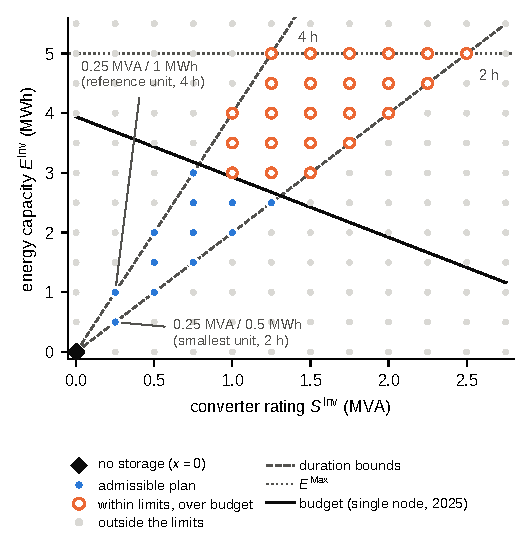
\includegraphics[width=0.75\textwidth]{fig_lattice_case.pdf}
    \caption{Admissible single-node investment plans for installation in 2025 under the baseline constraints. The investment budget is shared across all nodes.}
    \label{fig:investment_lattice}
\end{figure}
\DIFaddend 


    \DIFdelbegin %DIFDELCMD < \begin{figure*}[htbp]
%DIFDELCMD <     \centering
%DIFDELCMD <     \subfloat[Spring 2025]{
%DIFDELCMD <         \includegraphics[width=0.475\textwidth]{case33_2_load_scenarios_2025_Spring.pdf}
%DIFDELCMD <     }
%DIFDELCMD <     \hfill
%DIFDELCMD <     \subfloat[Summer 2025]{
%DIFDELCMD <         \includegraphics[width=0.475\textwidth]{case33_2_load_scenarios_2025_Summer.pdf}
%DIFDELCMD <     }
%DIFDELCMD <     \\[5pt]
%DIFDELCMD <     \subfloat[Autumn 2025]{
%DIFDELCMD <         \includegraphics[width=0.475\textwidth]{case33_2_load_scenarios_2025_Autumn.pdf}
%DIFDELCMD <     }
%DIFDELCMD <     \hfill
%DIFDELCMD <     \subfloat[Winter 2025]{
%DIFDELCMD <         \includegraphics[width=0.475\textwidth]{case33_2_load_scenarios_2025_Winter.pdf}
%DIFDELCMD <     }
%DIFDELCMD <     \caption{ADN at TN node 7: load profiles for 2025.}
%DIFDELCMD <     \label{fig:cs3_adn_node_7_load_scenarios_2025}
%DIFDELCMD < \end{figure*}
%DIFDELCMD < %%%
\DIFdelend \DIFaddbegin \DIFadd{The planning search evaluated all fourteen admissible unit neighbours of the plan without storage at its own resolution ($\sigma_Q$, or the sum of the two evaluations' bars where larger; Subsection~\ref{subsec:res_baseline}). Table~\ref{tab:appE_neighbours} gives the eight of them that were re-evaluated under the certification rule: the smallest unit, 0.25~MVA / 0.5~MWh, at each node installed in 2025 or 2030, and at two pairs of nodes. Every one costs determinately more than the plan without storage. The other six, the smallest unit at the two remaining pairs of nodes and at all three nodes, in 2025 or 2030, were evaluated by the search only, on an earlier state of the code and stopped by the production exit; each cost more than the plan without storage by 3.47--7.17 times the search resolution.
}\DIFaddend 


\DIFdelbegin %DIFDELCMD < \begin{figure}[htbp!]
%DIFDELCMD <     \centering
%DIFDELCMD <     \includegraphics[width=0.65\textwidth]{case33_2_flexibility_scenarios_2025_Spring.pdf}
%DIFDELCMD <     \caption{Flexible load profiles for the ADN at TN node~7.}
%DIFDELCMD <     \label{fig:cs3_adn_node_7_flexibility}
%DIFDELCMD < \end{figure}
%DIFDELCMD < %%%
\DIFdelend \DIFaddbegin \begin{table}[htbp!]
    \centering
    \caption{Neighbours of the plan without storage re-evaluated under the certification rule: the smallest unit (0.25~MVA / 0.5~MWh) at the nodes listed. $\Delta = F(\boldsymbol{x}) - F(\boldsymbol{0})$, gross operational cost, contracted interface settlement excluded; every difference is determinate.}
    \label{tab:appE_neighbours}
    \scriptsize\setlength{\tabcolsep}{5pt}
    \begin{tabular}{l c c r r r}
        \toprule
        Node(s) & Year & Eval. & $\Delta$ (k\euro) & Threshold (k\euro) & $\times$ \\
        \midrule
        5 & 2025 & 15 & 49.7 & 12.6 & 3.94 \\
        7 & 2025 & 17 & 54.9 & 13.3 & 4.14 \\
        9 & 2025 & 18 & 52.5 & 12.6 & 4.15 \\
        5 & 2030 & 19 & 43.3 & 12.7 & 3.40 \\
        7 & 2030 & 20 & 49.0 & 13.5 & 3.62 \\
        9 & 2030 & 21 & 46.7 & 12.8 & 3.64 \\
        5 and 9 & 2025 & 22 & 102.1 & 12.6 & 8.09 \\
        5 and 7 & 2030 & 23 & 93.9 & 13.4 & 7.00 \\
        \bottomrule
    \end{tabular}
    \par\smallskip
    \begin{minipage}{0.80\linewidth}
        \scriptsize\raggedright
        \textit{Note:} The superseded first certificate of the 2025 node-5 neighbour (evaluation~16) gave 51.3~k\euro{} (3.79$\times$).
    \end{minipage}
\end{table}
\DIFaddend 

\DIFdelbegin \subsection{\DIFdel{ADN Connected to TN node~9}}
%DIFAUXCMD
\addtocounter{subsection}{-1}%DIFAUXCMD
%DIFDELCMD < \label{app:adn_node9_description}
%DIFDELCMD < %%%
\DIFdelend \DIFaddbegin \subsection{\DIFadd{Certification Statistics and Reproducibility}}
\label{app:results_statistics}
\DIFaddend 


    \DIFdelbegin \DIFdel{Figure~[\texttt{fig:cs3\_adn\_node\_9\_res\_scenarios\_2025}] and Figure~[\texttt{fig:cs3\_adn\_node\_9\_load\_scenarios\_2025}] show the RES generation and load profiles for the spring, summer, autumn, and winter representative days of 2025 for the ADN at TN node~9. Figure~[\texttt{fig:cs3\_adn\_node\_9\_flexibility}] shows the flexible load profiles adopted for this ADN. }\DIFdelend \DIFaddbegin \DIFadd{The three planning searches used earlier versions of the implementation without the tightened interior-point tolerances used for numerical acceptance. Their reported incumbents were re-evaluated using the settings in~\ref{app:admm_updated_settings}.
}\DIFaddend 



    \DIFdelbegin %DIFDELCMD < \begin{figure*}[htbp]
%DIFDELCMD <     \centering
%DIFDELCMD <     \subfloat[Spring 2025]{
%DIFDELCMD <         \includegraphics[width=0.475\textwidth]{case33_3_RES_generation_scenarios_2025_Spring.pdf}
%DIFDELCMD <     }
%DIFDELCMD <     \hfill
%DIFDELCMD <     \subfloat[Summer 2025]{
%DIFDELCMD <         \includegraphics[width=0.475\textwidth]{case33_3_RES_generation_scenarios_2025_Summer.pdf}
%DIFDELCMD <     }
%DIFDELCMD <     \\[5pt]
%DIFDELCMD <     \subfloat[Autumn 2025]{
%DIFDELCMD <         \includegraphics[width=0.475\textwidth]{case33_3_RES_generation_scenarios_2025_Autumn.pdf}
%DIFDELCMD <     }
%DIFDELCMD <     \hfill
%DIFDELCMD <     \subfloat[Winter 2025]{
%DIFDELCMD <         \includegraphics[width=0.475\textwidth]{case33_3_RES_generation_scenarios_2025_Winter.pdf}
%DIFDELCMD <     }
%DIFDELCMD <     \caption{ADN at TN node 9: RES profiles for 2025.}
%DIFDELCMD <     \label{fig:cs3_adn_node_9_res_scenarios_2025}
%DIFDELCMD < \end{figure*}
%DIFDELCMD < %%%
\DIFdelend \DIFaddbegin \DIFadd{The acceptance tolerance~\eqref{eq:acceptance_tolerance} uses $\delta_R = 0.07$ on the reference value $\mathcal{V} = 259{,}375.33$~}\euro{}\DIFadd{, the value of the reference unit in force when the rule was adopted, hence $\tau = 4{,}539.07$~}\euro{}\DIFadd{, kept frozen thereafter, and $P_{\max} = 30$ cycles;
    an evaluation continued from, or re-run on, an earlier record is capped 100 cycles after that record's stopping cycle, a fresh one at $\min\{k_0 + 109, 300\}$. The planning search (Algorithm~\ref{alg:shared_ess_planning_mads}) used $\Delta_0 = 4$ lattice units, budgets of 20 new evaluations for the two variant-A searches and 60 for the variant-B certificate, a completion cap of 30 points, and the measured resolution $\sigma_Q = 18{,}449.66$~}\euro{} \DIFadd{of the recourse.
    The search evaluations ran under the production exit (ten consecutive passing cycles, cap 500 cycles); variant B polled at unit size throughout; a run was stopped for review when a completion set exceeded the cap or when two barrier points occurred in one poll or three in all, and ran at most 60 polls; the cache of the baseline search was seeded with the single-node ladders of the initial design, including ladder points over the budget, and the caches of the two searches under the doubled flexibility price with the certified evaluations at that price, which for the variant-B run include multi-node plans installed in 2030.
}\DIFaddend 



    \DIFdelbegin %DIFDELCMD < \begin{figure*}[htbp]
%DIFDELCMD <     \centering
%DIFDELCMD <     \subfloat[Spring 2025]{
%DIFDELCMD <         \includegraphics[width=0.475\textwidth]{case33_3_load_scenarios_2025_Spring.pdf}
%DIFDELCMD <     }
%DIFDELCMD <     \hfill
%DIFDELCMD <     \subfloat[Summer 2025]{
%DIFDELCMD <         \includegraphics[width=0.475\textwidth]{case33_3_load_scenarios_2025_Summer.pdf}
%DIFDELCMD <     }
%DIFDELCMD <     \\[5pt]
%DIFDELCMD <     \subfloat[Autumn 2025]{
%DIFDELCMD <         \includegraphics[width=0.475\textwidth]{case33_3_load_scenarios_2025_Autumn.pdf}
%DIFDELCMD <     }
%DIFDELCMD <     \hfill
%DIFDELCMD <     \subfloat[Winter 2025]{
%DIFDELCMD <         \includegraphics[width=0.475\textwidth]{case33_3_load_scenarios_2025_Winter.pdf}
%DIFDELCMD <     }
%DIFDELCMD <     \caption{ADN at TN node 9: load profiles for 2025.}
%DIFDELCMD <     \label{fig:cs3_adn_node_9_load_scenarios_2025}
%DIFDELCMD < \end{figure*}
%DIFDELCMD < %%%
\DIFdelend \DIFaddbegin \DIFadd{The baseline search used variant A and performed 14 new recourse evaluations. The initial search at twice the base flexibility price also used variant A and performed 20 new evaluations; it stopped when the unit-neighbour completion set exceeded the cap. A variant-B search continued from its incumbent and performed seven new evaluations. All new evaluations in the variant-A searches came from unit-neighbour completion. The baseline and variant-B searches stopped after unsuccessful unit polls.
}\DIFaddend 



    \DIFdelbegin %DIFDELCMD < \begin{figure}[htbp!]
%DIFDELCMD <     \centering
%DIFDELCMD <     \includegraphics[width=0.65\textwidth]{case33_3_flexibility_scenarios_2025_Spring.pdf}
%DIFDELCMD <     \caption{Flexible load profiles for the ADN at TN node~9.}
%DIFDELCMD <     \label{fig:cs3_adn_node_9_flexibility}
%DIFDELCMD < \end{figure}
%DIFDELCMD < %%%
\DIFdelend \DIFaddbegin \DIFadd{At every certificate used in a reported comparison, and at both multi-scenario evaluations, both daily closure slacks sat at their lower bound to within the solver's bound relaxation ($10^{-6}$~MWh per slack); in the superseded evaluation~16 of Table~S4 their sum reached $1.8 \times 10^{-6}$~MWh, $5 \times 10^{-6}$ of the available energy. Without storage the closure row is deactivated and its slacks are fixed at zero.
    The shared-ESS agent's net-active-power slacks $\sigma^\pm_{e,y,d,t}$ were at their lower bounds at every certified evaluation.
    More generally, at every certified evaluation behind the tables of Section~\ref{sec:results}, every penalised slack in $Q$ (daily closure and network feasibility) sits at its zero bound to within the solver's bound relaxation, so no penalty is paid in $Q$, and the agent's net-power pair, penalised in the agent's own objective, is at its bound as well; the relaxation itself leaves a common offset of $-13.0$~k}\euro{} \DIFadd{in $Q$ ($-2 \times 10^{-5}$ of $Q$), identical across evaluations to within 40~}\euro{}\DIFadd{, which cancels in every reported difference. The multi-scenario evaluation of the reference unit carries a positive flexibility-balance content of at most 2.2~}\euro{}\DIFadd{, and the superseded evaluation~16 a positive slack content of at most 171~}\euro{}\DIFadd{, almost all of it voltage slack.
}\DIFaddend 



    \DIFdelbegin \section{\DIFdel{Results}}
%DIFAUXCMD
\addtocounter{section}{-1}%DIFAUXCMD
%DIFDELCMD < \label{app:results}
%DIFDELCMD < 

%DIFDELCMD < %%%
\DIFdel{Table~[\texttt{tab:cs3\_results\_summary\_years\_days}] provides a detailed breakdown of operational costs, RES generation, }\DIFdelend \DIFaddbegin \textbf{\DIFadd{Certification statistics.}} \DIFadd{The 42 single-scenario evaluations of the certification campaign are evaluations 3--11, 15, 22, 23, 26--31, 34--39 }\DIFaddend and \DIFdelbegin \DIFdel{RES curtailment for each representative year and season. It complements the aggregated results reported in Section~\ref{sec:results} and enables a more granular assessment of seasonal and inter-annual performance differences across test cases. }\DIFdelend \DIFaddbegin \DIFadd{42--59 of Table~S4. Of these, 32 certified, 24 on the oscillatory branch and 8 on the monotone branch; the 10 uncertified divide into 5 refused by the gap clause, 2 reset by residual lapses and 3 failed by the growth test. The median certification cycle was 174, and certification came a median 65 cycles after the first residual pass (range 21--89); the median ratio of the window range to $\tau$ at certification was 0.86. The four evaluations added later (32, 33, 60 and 61) all certified. Ten of the 46 certificates the tables use stop within 5\,\% of $\tau$ (evaluations 2, 3, 5, 10, 11, 12, 14, 17, 20 and 23; evaluation~36, at 0.94 on the monotone branch, is just below), so the accepted window ranges can lie close to $\tau$, without providing a guaranteed bound on the remaining objective movement. The three evaluations continued past their certificates, 12, 14 and 3, moved by a further 0.004$\tau$, 0.74$\tau$ and 0.78--0.88$\tau$. After the first residual pass, 21 cycles in 10 evaluations had a local solve that was not clean, all in transmission blocks (column N.c.), while the 119 exits at IPOPT's acceptable level within ten times the tight-tail tolerances, all in distribution blocks, were counted as clean.
}\DIFaddend 



    \DIFdelbegin %DIFDELCMD < \begin{landscape}
%DIFDELCMD <     \begin{table}[htbp!]
%DIFDELCMD <     \centering
%DIFDELCMD <     \caption{Operational planning results by representative year and representative day.}
%DIFDELCMD <     \resizebox{1.40\textwidth}{!}{
%DIFDELCMD <         \begin{tabular}{lll cccc c cccc c cccc c cccc c cccc}
%DIFDELCMD <             \toprule
%DIFDELCMD <             ~ & ~ & ~ & \multicolumn{4}{c}{2025} & ~ & \multicolumn{4}{c}{2028} & ~ & \multicolumn{4}{c}{2031} & ~ & \multicolumn{4}{c}{2034} & ~ & \multicolumn{4}{c}{2037}\\
%DIFDELCMD <             \cmidrule{4-7} \cmidrule{9-12} \cmidrule{14-17} \cmidrule{19-22} \cmidrule{24-27}
%DIFDELCMD <             ~ & ~ & ~ & Spring & Summer & Autumn & Winter &  
%DIFDELCMD <                       & Spring & Summer & Autumn & Winter &  
%DIFDELCMD <                       & Spring & Summer & Autumn & Winter & 
%DIFDELCMD <                       & Spring & Summer & Autumn & Winter & 
%DIFDELCMD <                       & Spring & Summer & Autumn & Winter \\
%DIFDELCMD <             \midrule
%DIFDELCMD <             \multicolumn{3}{l}{Uncoordinated}\\ \cmidrule{2-27}
%DIFDELCMD <             ~ & \multicolumn{2}{l}{Operational Cost, [\euro]}   & 269671.54 & 240359.85 & 194686.35 & 207466.96 & ~
%DIFDELCMD <                                                                 & 278745.92 & 271843.10 & 239972.27 & 247310.67 & ~
%DIFDELCMD <                                                                 & 266821.42 & 241056.10 & 178945.77 & 159305.51 & ~
%DIFDELCMD <                                                                 & 313102.26 & 288405.93 & 179448.50 & 209415.34 & ~
%DIFDELCMD <                                                                 & 329528.87 & 294022.70 & 195895.18 & 275763.44\\
%DIFDELCMD <             ~ & \multicolumn{2}{l}{RES Generation, [MWh]}       & 814.83 & 875.19 & 907.46 & 1074.27 & ~
%DIFDELCMD <                                                                 & 799.59 & 871.78 & 1038.93 & 1140.19 & ~
%DIFDELCMD <                                                                 & 1170.76 & 1106.34 & 1547.14 & 1573.34 & ~
%DIFDELCMD <                                                                 & 1227.64 & 1206.71 & 1462.45 & 1631.29 & ~
%DIFDELCMD <                                                                 & 1177.36 & 927.30 & 1831.44 & 1322.29\\
%DIFDELCMD <             ~ & \multicolumn{2}{l}{RES Curtailment, [MVAh]}     & 0.00 & 5.22 & 0.00 & 0.00 & ~
%DIFDELCMD <                                                                 & 10.98 & 0.00 & 0.00 & 0.00 & ~
%DIFDELCMD <                                                                 & 84.56 & 240.34 & 0.00 & 0.00 & ~
%DIFDELCMD <                                                                 & 57.84 & 159.49 & 0.00 & 0.00 & ~
%DIFDELCMD <                                                                 & 316.18 & 697.68 & 0.00 & 624.33\\
%DIFDELCMD <             \midrule
%DIFDELCMD <             \multicolumn{3}{l}{Without Shared ESSs}\\ \cmidrule{2-27}
%DIFDELCMD <             ~ & \multicolumn{2}{l}{Operational Cost}\\       
%DIFDELCMD <             ~ & ~ & Total, [\euro]  & 244253.20 & 235518.58 & 200807.07 & 208417.00 & ~
%DIFDELCMD <                                     & 248518.89 & 259801.27 & 245425.14 & 249162.75 & ~ 
%DIFDELCMD <                                     & 231386.32 & 229083.91 & 184500.25 & 162710.69 & ~ 
%DIFDELCMD <                                     & 274169.86 & 272988.69 & 187791.61 & 211915.70 & ~
%DIFDELCMD <                                     & 270509.42 & 247965.68 & 205275.47 & 189951.70\\
%DIFDELCMD <             ~ & ~ & Variation, [\%] & -9.43\% & -2.01\% & 3.14\% & 0.46\% & ~ 
%DIFDELCMD <                                     & -10.84\% & -4.43\% & 2.27\% & 0.75\% & ~
%DIFDELCMD <                                     & -13.28\% & -4.97\% & 3.10\% & 2.14\% & ~ 
%DIFDELCMD <                                     & -12.43\% & -5.35\% & 4.65\% & 1.19\% & ~
%DIFDELCMD <                                     & -17.91\% & -15.66\% & 4.79\% & -31.12\%\\ \cmidrule{2-27}
%DIFDELCMD <             ~ & \multicolumn{2}{l}{RES Generation}\\
%DIFDELCMD <             ~ & ~ & Total, [MWh] & 795.04 & 867.14 & 894.16 & 1076.33 & ~
%DIFDELCMD <                                  & 773.76 & 856.18 & 1025.98 & 1137.93 & ~ 
%DIFDELCMD <                                  & 1218.67 & 1335.05 & 1538.91 & 1569.59 & ~ 
%DIFDELCMD <                                  & 1259.00 & 1353.06 & 1451.31 & 1626.96 & ~
%DIFDELCMD <                                  & 1405.13 & 1537.88 & 1825.09 & 1944.63\\
%DIFDELCMD <             ~ & ~ & Variation, [\%] & -2.43\% & -0.92\% & -1.47\% & 0.19\% & ~ 
%DIFDELCMD <                                     & -3.23\% & -1.79\% & -1.25\% & -0.20\% & ~ 
%DIFDELCMD <                                     & 4.09\% & 20.67\% & -0.53\% & -0.24\% & ~ 
%DIFDELCMD <                                     & 2.56\% & 12.13\% & -0.76\% & -0.27\% & ~ 
%DIFDELCMD <                                     & 19.35\% & 65.85\% & -0.35\% & 47.07\%\\
%DIFDELCMD <             \cmidrule{2-27}
%DIFDELCMD <             ~ & \multicolumn{2}{l}{RES Curtailment}\\       
%DIFDELCMD <             ~ & ~ & Total, [MVAh]  & 19.76 & 13.29 & 13.25 & 5.41 & ~ 
%DIFDELCMD <                                   & 36.80 & 15.56 & 12.90 & 5.79 & ~ 
%DIFDELCMD <                                   & 36.66 & 12.18 & 8.19 & 3.70 & ~
%DIFDELCMD <                                   & 26.48 & 13.21 & 11.10 & 4.29 & ~
%DIFDELCMD <                                   & 88.47 & 87.80 & 7.13 & 3.72\\
%DIFDELCMD <             ~ & ~ & Variation, [\%] & N/A & 154.45\% & N/A & N/A & ~ 
%DIFDELCMD <                                     & 235.22\% & N/A & N/A & N/A & ~ 
%DIFDELCMD <                                     & -56.65\% & -94.93\% & N/A & N/A & ~
%DIFDELCMD <                                     & -54.22\% & -91.72\% & N/A & N/A & ~
%DIFDELCMD <                                     & -72.02\% & -87.42\% & N/A & -99.40\%\\
%DIFDELCMD <             \midrule
%DIFDELCMD <             \multicolumn{3}{l}{With Shared ESSs}\\ \cmidrule{2-27}
%DIFDELCMD <             ~ & \multicolumn{2}{l}{Operational Cost}\\   
%DIFDELCMD <             ~ & ~ & Total, [\euro]  & 244140.90 & 234804.95 & 200439.69 & 209948.35 & ~
%DIFDELCMD <                                     & 246055.36 & 258220.48 & 245809.26 & 249029.65 & ~ 
%DIFDELCMD <                                     & 233458.63 & 227967.81 & 186566.71 & 160903.39 & ~ 
%DIFDELCMD <                                     & 284765.82 & 272862.03 & 187353.93 & 212285.38 & ~ 
%DIFDELCMD <                                     & 269546.16 & 233501.93 & 203314.34 & 188930.78\\
%DIFDELCMD <             ~ & ~ & Variation, [\%] & -9.47\% & -2.31\% & 2.96\% & 1.20\% & ~ 
%DIFDELCMD <                                     & -11.73\% & -5.01\% & 2.43\% & 0.70\% & ~
%DIFDELCMD <                                     & -12.50\% & -5.43\% & 4.26\% & 1.00\% & ~ 
%DIFDELCMD <                                     & -9.05\% & -5.39\% & 4.41\% & 1.37\% & ~ 
%DIFDELCMD <                                     & -18.20\% & -20.58\% & 3.79\% & -31.49\%\\ \cmidrule{2-27}
%DIFDELCMD <             ~ & \multicolumn{2}{l}{RES Generation}\\       
%DIFDELCMD <             ~ & ~ & Total, [MWh] & 795.03 & 867.15 & 894.17 & 1076.34 & ~ 
%DIFDELCMD <                                  & 773.74 & 856.20 & 1025.95 & 1137.90 & ~ 
%DIFDELCMD <                                  & 1218.68 & 1334.90 & 1538.84 & 1569.55 & ~ 
%DIFDELCMD <                                  & 1212.29 & 1353.10 & 1451.27 & 1626.96 & ~ 
%DIFDELCMD <                                  & 1405.29 & 1597.11 & 1825.09 & 1944.64\\
%DIFDELCMD <             ~ & ~ & Variation, [\%] & -2.43\% & -0.92\% & -1.47\% & 0.19\% & ~
%DIFDELCMD <                                     & -3.23\% & -1.79\% & -1.25\% & -0.20\% & ~
%DIFDELCMD <                                     & 4.09\% & 20.66\% & -0.54\% & -0.24\% & ~
%DIFDELCMD <                                     & -1.25\% & 12.13\% & -0.76\% & -0.27\% & ~
%DIFDELCMD <                                     & 19.36\% & 72.23\% & -0.35\% & 47.07\%\\ \cmidrule{2-27}
%DIFDELCMD <             ~ & \multicolumn{2}{l}{RES Curtailment}\\       
%DIFDELCMD <             ~ & ~ & Total, [MVAh] & 19.77 & 13.28 & 13.25 & 5.41 & ~
%DIFDELCMD <                                   & 36.82 & 15.55 & 12.87 & 5.78 & ~
%DIFDELCMD <                                   & 36.63 & 12.30 & 8.21 & 3.75 & ~
%DIFDELCMD <                                   & 73.17 & 13.16 & 11.14 & 4.29 & ~
%DIFDELCMD <                                   & 88.31 & 28.58 & 7.12 & 3.70\\
%DIFDELCMD <             ~ & ~ & Variation, [\%] & N/A & 154.19\% & N/A & N/A & ~
%DIFDELCMD <                                     & 235.43\% & N/A & N/A & N/A & ~
%DIFDELCMD <                                     & -56.68\% & -94.88\% & N/A & N/A & ~
%DIFDELCMD <                                     & 26.49\% & -91.75\% & N/A & N/A & ~
%DIFDELCMD <                                     & -72.07\% & -95.90\% & N/A & -99.41\%\\
%DIFDELCMD <             \bottomrule
%DIFDELCMD <         \end{tabular}
%DIFDELCMD <     }
%DIFDELCMD <     \label{tab:cs3_results_summary_years_days}
%DIFDELCMD <     \end{table}
%DIFDELCMD < \end{landscape}
%DIFDELCMD < %%%
\DIFdelend \DIFaddbegin \textbf{\DIFadd{Reproducibility.}} \DIFadd{Replaying a run reproduces its trajectory bitwise: the multi-scenario evaluation of the plan without storage replayed its 72 recorded cycles bitwise; the three single-scenario reference continuations (the plan without storage, the reference unit and a larger plan not tabulated here) replayed bitwise through the stopping cycles of the residual-based runs they continue, cycles 132, 112 and 87; and every evaluation repeated from an earlier record replayed that record bitwise up to its first residual pass before continuing (column Replay). The evaluations ran one at a time on an Apple M2~Max with 32~GiB of memory under macOS~27.0, single-threaded: OMP, MKL, OpenBLAS, vecLib and NumExpr were capped at one thread in every evaluation's recorded environment, and the HSL library is built without OpenMP, so MA97 ran serially; the solver settings and versions are listed in~\ref{app:admm_updated_settings}. Two distribution blocks (node~7 in 2025 Winter, node~5 in 2035 Winter) end some primary solves at IPOPT's acceptable level within ten times the tight-tail tolerances; they are counted as clean under the rule of~\ref{app:admm_updated_certification}. Two offsets are common to every evaluation and cancel in every reported difference: tightening the interior-point tail lowered the certified objective of each of the three single-scenario references by $1.0$--$1.2 \times 10^{-6}$ relative, with the same sign (the complementarity tolerance went to $10^{-6}$ from $10^{-4}$ in the distribution subproblems and from $5 \times 10^{-4}$ in the transmission subproblem); and the $10^{-5}$~p.u. slack on the renewable availability bound lowers the objective by about 7.8~k}\euro{} \DIFadd{at first order, $1.2 \times 10^{-5}$ of it.
}\DIFaddend 



\section*{Declaration of generative AI and AI-assisted technologies in the manuscript preparation process}

During the preparation of this work the author(s) used ChatGPT in order to improve readability and language in selected parts of the manuscript. After using this tool, the author(s) reviewed and edited the content as needed and take full responsibility for the content of the published article.

% ====================================================================================================================
%                                                     BIBLIOGRAPHY                                                    
% ====================================================================================================================
\bibliographystyle{elsarticle-num} 
\bibliography{bibliography}

\end{document}

\endinput
%%
%% End of file `elsarticle-template-num.tex'.
